\chapter{Sensitivity of the SuperNEMO demonstrator to the $\zeronu$}
\label{ch:sensitivity}

A study aiming to evaluate the SuperNEMO sensitivity to the $\zeronu$ decay, and the corresponding effective neutrino mass is presented.
The final detector, based on the NEMO-$3$ technology, is expected to exclude half-lives up to $1\times 10^{26}$~y ($90\%$ CL), with an exposure of $500$~kg.y with Selenium sources\footnote{Supposing the $\zeronu$ decay of \Se\ occurs through the exchange of a light Majorana neutrino.}~\cite{art:SuperNEMO2010}.
The SuperNEMO demonstrator was designed in order to assess the technical feasibility of such a large-scale detector and to show that background specifications can be achieved.
Its installation started in early $2015$, at the Laboratoire Souterrain de Modane.
With a reduced exposure of $17.5$~kg.y, this demonstrator is expected to reach a sensitivity on the $\zeronu$ process of $5.3\times~10^{24}$~y ($90\%$ CL)~\cite{CalvezThesis}.

As it was the case with its predecessor, a copper coil was designed to deliver a magnetic field inside the wire chamber, to bend the charged particles trajectories, hence making it possible to discriminate between electrons and positrons.
However, studies led by the collaboration determined that this field could be impacted by the photomultiplier magnetic shields, producing notable variations in intensity and a loss of energy resolution~\cite{CalvezThesis,internal:magnetic_field}.
We aim to explore the impact, on both the demonstrator and final detector sensitivity, of the presence of this magnetic field.
The findings of this study participate in better understanding the detector performances.
In a context of investigating the demonstrator and final detector's capabilities, different internal source contamination levels are considered.
The topology of interest is that of two electrons, and we use the total energy sum to discriminate the signal from the background events.
Thanks to SuperNEMO tracking capabilities, extra topological informations are exploited to improve the final sensitivity.
To go further, we also explore the possibility of studying the $\zeronu$ decay of other $\beta\beta$ isotopes.

\section{The $\zeronu$ signal and background model}
\label{sec:sensitivity_simus}

A full GEANT$4$ simulation of the demonstrator was performed to determine, the lower limit on the $\zeronu$ half-life that can be probed with SuperNEMO in case of the non-observation of the signal.
Due to the time it would take to simulate every background contribution, we choose a simplified model.
Indeed, only the most harmful backgrounds to the $\zeronu$ decay search were simulated.
In addition, $\zeronu$ signal decays inside the detector were simulated, to better understand all the aspects of this analysis.

\subsection{The $\zeronu$ signal}

The SuperNEMO detector was designed to search for the yet never-observed $\zeronu$ decay.
In the following, we assume the underlying mechanism for this decay is the exchange of a light Majorana neutrino, the so-called mass mechanism (MM), as it is the most widespread.
The hypothetical $\zeronu$ signal would be detected as an excess of events at the end point of the $\twonu$ spectrum, with respect to the predicted background contamination levels.
Some $10^{7}$ $\zeronu$ events were simulated inside the source foils, using the DECAY$0$ software~\cite{art:decay0}.

\subsection{Inside detector backgrounds}

Nnumerous types of backgrounds that could mimic and hinder the search for the $\zeronu$ signal were simulated.

\subsubsection{Internal backgrounds}

The so-called \emph{internal backgrounds} stand for decays occurring inside the source foils, presenting the same signature as the $\zeronu$ signal.
These backgrounds are mainly the $\twonu$ decay undergone by the source isotope, disintegrations of \Tl\ and \Bi\ contaminations inside the source foils, as well as \Bi\ disintegrations due to Radon deposited on the surface of the source foils.

\subsubsection*{The $\twonu$ process}

In the full energy range, the allowed $\twonu$ decay of \Se\ stands as the dominant internal background type.
The corresponding two-electrons energy sum spectrum is a continuum, whose ending point should stands at $\Qbb = 2.99$~MeV, but is subtly shifted by the detector's energy resolution due to energy losses inside the source foils and gaseous detector.
A total of $10^{7}$ events of this decay were simulated inside the source foils, in the full energy window.
However, above a certain energy value, the number of $\twonu$ events decreases strongly, which can lead to a lack of statistics in a energy region favourable for the search for $\zeronu$ signal.
To offset this effect, additional $10^{7}$ of this decay were simulated on a slightly reduced energy range, that is to say above $2$~MeV.
The second set of simulations is normalised with the first one.
In this way, the lack of $\twonu$ simulated events in the high-energy tail is avoided, without requiring too high computational resources.

\subsubsection*{Source foils contamination by natural isotopes}

As described in Sec.~\ref{subsec:SNbkg_internal}, after sources purification, residual natural isotopes such as \Tl\ or \Bi\ can still be present inside the foils, constituting the principal internal source of background, with the $\twonu$ decay.
A total of $10^{7}$ decays for each of the two isotopes were simulated inside the source foils.

\subsubsection{Tracker contamination by natural isotopes}

Radon, a descendant of \U, is present as a gas in the tracker.
Its daughter isotopes, when deposited on the tracker wires, can produce events similar to internal ones.
In fact, one of the progeny of \Rn, the \Bi, can decay on (or near) a foil, and appear with a two-electron topology, becoming hard to distinguish from a double beta decay candidate.
As this isotope is distributed throughout the whole tracking detection volume, a large quantity of this decay were simulated, that is to say $10^8$ decays on the tracker wires.
%This way, we maximise the amount of \Bi\ events, coming from \Rn\ decays, in the region of interest.


\subsection{External backgrounds}
\label{subsec:ext_bkg}

This background category was described in detail in Sec.~\ref{subsec:SNexternal_bkg}.
As a reminder, it is populated by the external $\gamma$-ray flux produced by radioactive isotope decays (mostly \K, \Bi\ and \Tl) in detector components or surrounding laboratory rocks, as well as neutron interactions in the external iron shield.
As simulating external backgrounds would be very consuming in terms of computing resources due to their very low probability to produce two electrons ($2e$) topologies, let us check that this source of background is negligible.
The NEMO-$3$ experiment set a limit on the external background number of counts, of $<0.2$ events in the $2e$ topology, for the energy range [$2.8$;$3.2$]~MeV (two electrons energy sum), for an exposure of $34.3$ kg·y, with $^{100}$Mo sources~\cite{art:NEMO2015}.
Recent radiopurity measurements of the SuperNEMO PMTs allow to conclude that the PMT \Bi\ activity is $35\%$ lower than for those of NEMO-$3$~\cite{docdb:perrot2017}, which is encouraging.
Unfortunately, these measurements also revealed that the PMT budget in \Tl\ isotope is $150\%$ higher than NEMO-$3$.
This could lead us to think that the external background contribution for SuperNEMO could be higher than that of NEMO-$3$.
However, on that level, the most notorious difference between the two detectors is the fact that the SuperNEMO scintillator blocks are thicker than those of NEMO-$3$.
Therefore, a gamma emitted from a PMT glass is more likely to be detected before crossing the source foils, such that it would be rejected and would not contribute to the background in the $2e$ channel.
Even if the regions of interest are slightly different between these two experiments, it produces a negligible increase on the external background contribution\footnote{A study conducted by the SuperNEMO collaboration showed that at most $0.73$ additional external background events would have been expected for the NEMO-$3$ detector, if instead of taking the [$2.8$;$3.2$]~MeV energy range, we would have considered the [$2.7$;$3.15$]~MeV region of interest.}.%%%%this limit is given by the stat simulated and could be ameliorated by more simulations by CPU
After all, given the fact that SuperNEMO is expected to be better than NEMO-$3$ at rejecting external background events, we consider that all external backgrounds from outside the foil, apart from \Rn\ in the tracking volume, are expected to be negligible, and were not simulated.

\subsection{Expected number of decays}

The number of natural isotope decay events expected in the $2e$ topology depends on their activities inside the source foils (for \Tl\ and \Bi), or on the tracker's wires (for \Rn\ decaying in \Bi).
Therefore, it is mandatory to constrain the maximal tolerable activities for the detector~\cite{internal:SNphysicsCase}.
The collaboration then established recommendations for maximum levels of the internal backgrounds, expressed in number of disintegrations per second, for a unit mass of $\beta\beta$ isotope, or for a unit volume of gas.
These \emph{specified activities} have been calculated in order to achieve the expected sensitivity of the final detector.

The amount of expected double $\beta$ decays is driven by its half-life value: the higher the half-life, the lower its contribution in the total number of expected background.
For this analysis, we consider the $\twonu$ half-life of \Se\ measured by NEMO-$3$, $\Ttwonu~=~9.39~\pm~0.17$~(stat)~$\pm~0.58$~(syst)~$\times~10^{19}$~years~\cite{art:NEMO2018}.
For the $\zeronu$ process, we also take the best limit set by the NEMO-$3$ detector, $\Tbeta > 2.5\times 10^{23}$~y~\cite{art:NEMO2018}.
This value is given for illustration purposes only, as it is not used to estimate the sensitivity of the detector.

Tab.~\ref{tab:sensitivity_simulations} gives the expected number of background events, for the demonstrator and final detector exposures, assuming target background activities are reached: $\mathcal{A}^{\text{Tl}}=10~\mu$Bq/kg, $\mathcal{A}^{\text{Bi}}=2~\mu$Bq/kg and $\mathcal{A}^{\text{Rn}}=0.15$~mBq/m$^{3}$.
\begin{table}[h!]
  \centering
  \begin{tabular}{|c|l|cc|}
    \hline
    Process & Half-life/Activity &\multicolumn{2}{c|}{Expected decays} \\
    && Demonstrator & Final detector \\
    \hline\hline
    $\twonu$ & $\Ttwonu = 9.39\times 10^{19}$ y & $9.5\times 10^{5}$ & $2.7\times 10^{7}$  \\
    \Tl\ & $\mathcal{A}^{\text{Tl}} = 2~\mu$Bq/kg  & $1.1\times 10^{3}$ & $3.1\times 10^{4}$  \\
    \Bi\ & $\mathcal{A}^{\text{Bi}} = 10~\mu$Bq/kg & $5.5\times 10^{3}$ & $1.6\times 10^{5}$ \\
    \Rn\ & $\mathcal{A}^{\text{Rn}} = 0.15$ mBq/m$^{3}$ & $1.8\times 10^{5}$ & $7.2\times 10^{6}$ \\
    \hline
  \end{tabular}
  \caption{Expected number of background events, for the demonstrator ($17.5$ kg.y) and for the final detector ($500$ kg.y).
    We assume target background activities are reached: $\mathcal{A}^{\text{Tl}}~=~10\,\mu$Bq/kg, $\mathcal{A}^{\text{Bi}}~=~2\,\mu$Bq/kg, $\mathcal{A}^{\text{Rn}}~=~0.15$ mBq/m$^{3}$.
    The measured half-life $\Ttwonu~=~9.39\times~10^{19}$ y for \Se\ is considered~\cite{art:NEMO2018}.
    \label{tab:sensitivity_simulations}}
\end{table}
The expected number of disintegrations do not take into account any technique to reject background, and are given for the full energy range of the two measured electrons.
Indeed, they are expected to be extremely reduced, notably by the application of event selections aimed at maximising the sensitivity to the $\zeronu$ half-life.
Moreover, for the current sensitivity analysis, we focus on a narrow energy window, called \emph{region of interest}, whose usefulness is described in detail in Sec.~\ref{sec:sensitivity_ev_selection}.
This is also one of the reasons why it was necessary to simulate a large number of events, so that the signal and backgrounds are correctly represented in the region of interest.


\section{Event selection}
\label{sec:sensitivity_ev_selection}

For SuperNEMO, the $\zeronu$ signature is two-electrons events, emitted simultaneously from the same vertex on the source foils, with an energy sum compatible with $\Qbb = 2.99$~MeV for \Se\ sources.
Therefore, we conducted this analysis selecting only events matching the $2e$ topology.

\subsection{Electron definition}

A reconstructed particle is tagged as an electron if it has:
\begin{itemize}
\item a vertex on the source foil,
\item a reconstructed track inside the wire chamber,
\item an associated calorimeter hit,
\item and a final criterion depending on the charged particle curvature.
\end{itemize}
About the last point, as announced, we aim at studying the influence of the magnetic field on the final sensitivity results.
To this end, we are led to consider two separate cases, one where the magnetic field is switched on, aligned with the $Z$ (vertical) axis of the detector, with a uniform value of $25$ Gauss, and one where it is switched off.
In the first case, particles such as electrons and positrons of a few~MeV have a curved trajectory in the tracker.
In the second case, the tracks of the particles may be similar to straight lines (not to mention the possible multiple scattering on the wires of the tracker).
It is then necessary to adapt the selection of events to each case.
When the magnetic field is on, we consider a fourth criterion: a particle is identified as an electron if its track has a negative curvature\footnote{A trajectory is said by convention to be negative if it has the same curvature as that of an electron moving from the source to the calorimeter, in a magnetic field oriented according to $+Z$.}.
In the following, we present results where the magnetic field is turned on.
The off-field study is addressed in Sec.~\ref{subsec:field}.

A two-electron ($2e$) topology is then defined as two reconstructed tracks with negative curvatures, each one associated with a vertex on the source foils and a calorimeter hit.
These selections represent the so-called \emph{first-order} cut-offs.
The $2e$ topologies have been selected using the Particle Identification module at the end of the Falaise reconstruction pipeline~\cite{CalvezThesis}.
I wrote my own module and added it to the collaboration software in order to store the selected events in a data format matching my off-line analysis chain.
Second order selections taking into account topological information (time of flight, location of vertices on the source foils) are presented in Sec.~\ref{sec:demonstrator_sensitivity}.

\subsection{Total energy spectrum}

In Fig.~\ref{fig:energy_spectra}, we present the total energy spectra for each simulated process in the $2e$ topology, after application of the first-order cut-offs.
\begin{figure}[h!]
\centering
\begin{subfigure}[t]{0.7\textwidth}
  \centering
  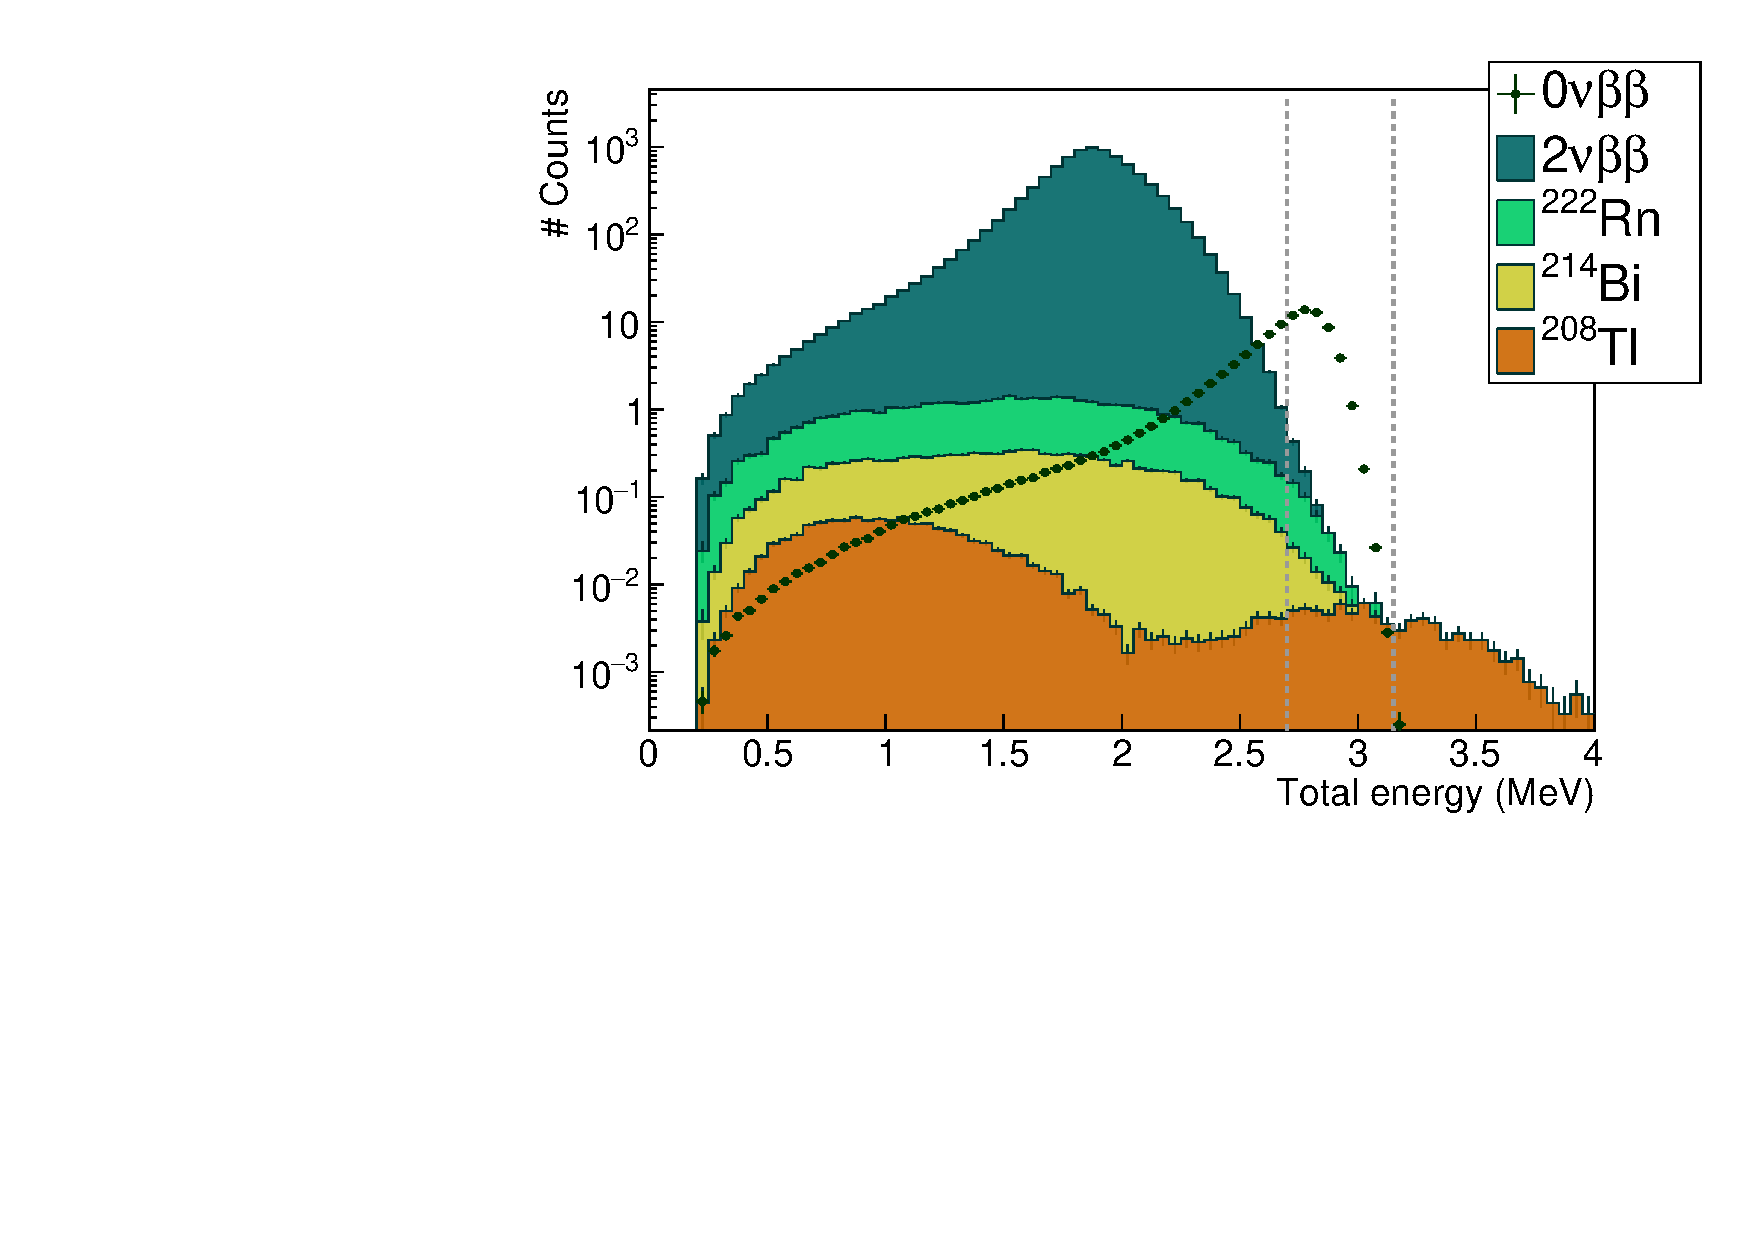
\includegraphics[width=1.1\textwidth]{Sensitivity/fig_sensitivity/energy_spectrum_with_B_82Se.pdf}
  \captionsetup{justification=centering}
  \caption{Full energy range.
    \label{subfig:energy_spectra_full}}
\end{subfigure}
\hfill
\begin{subfigure}[t]{0.7\textwidth}
  \centering
  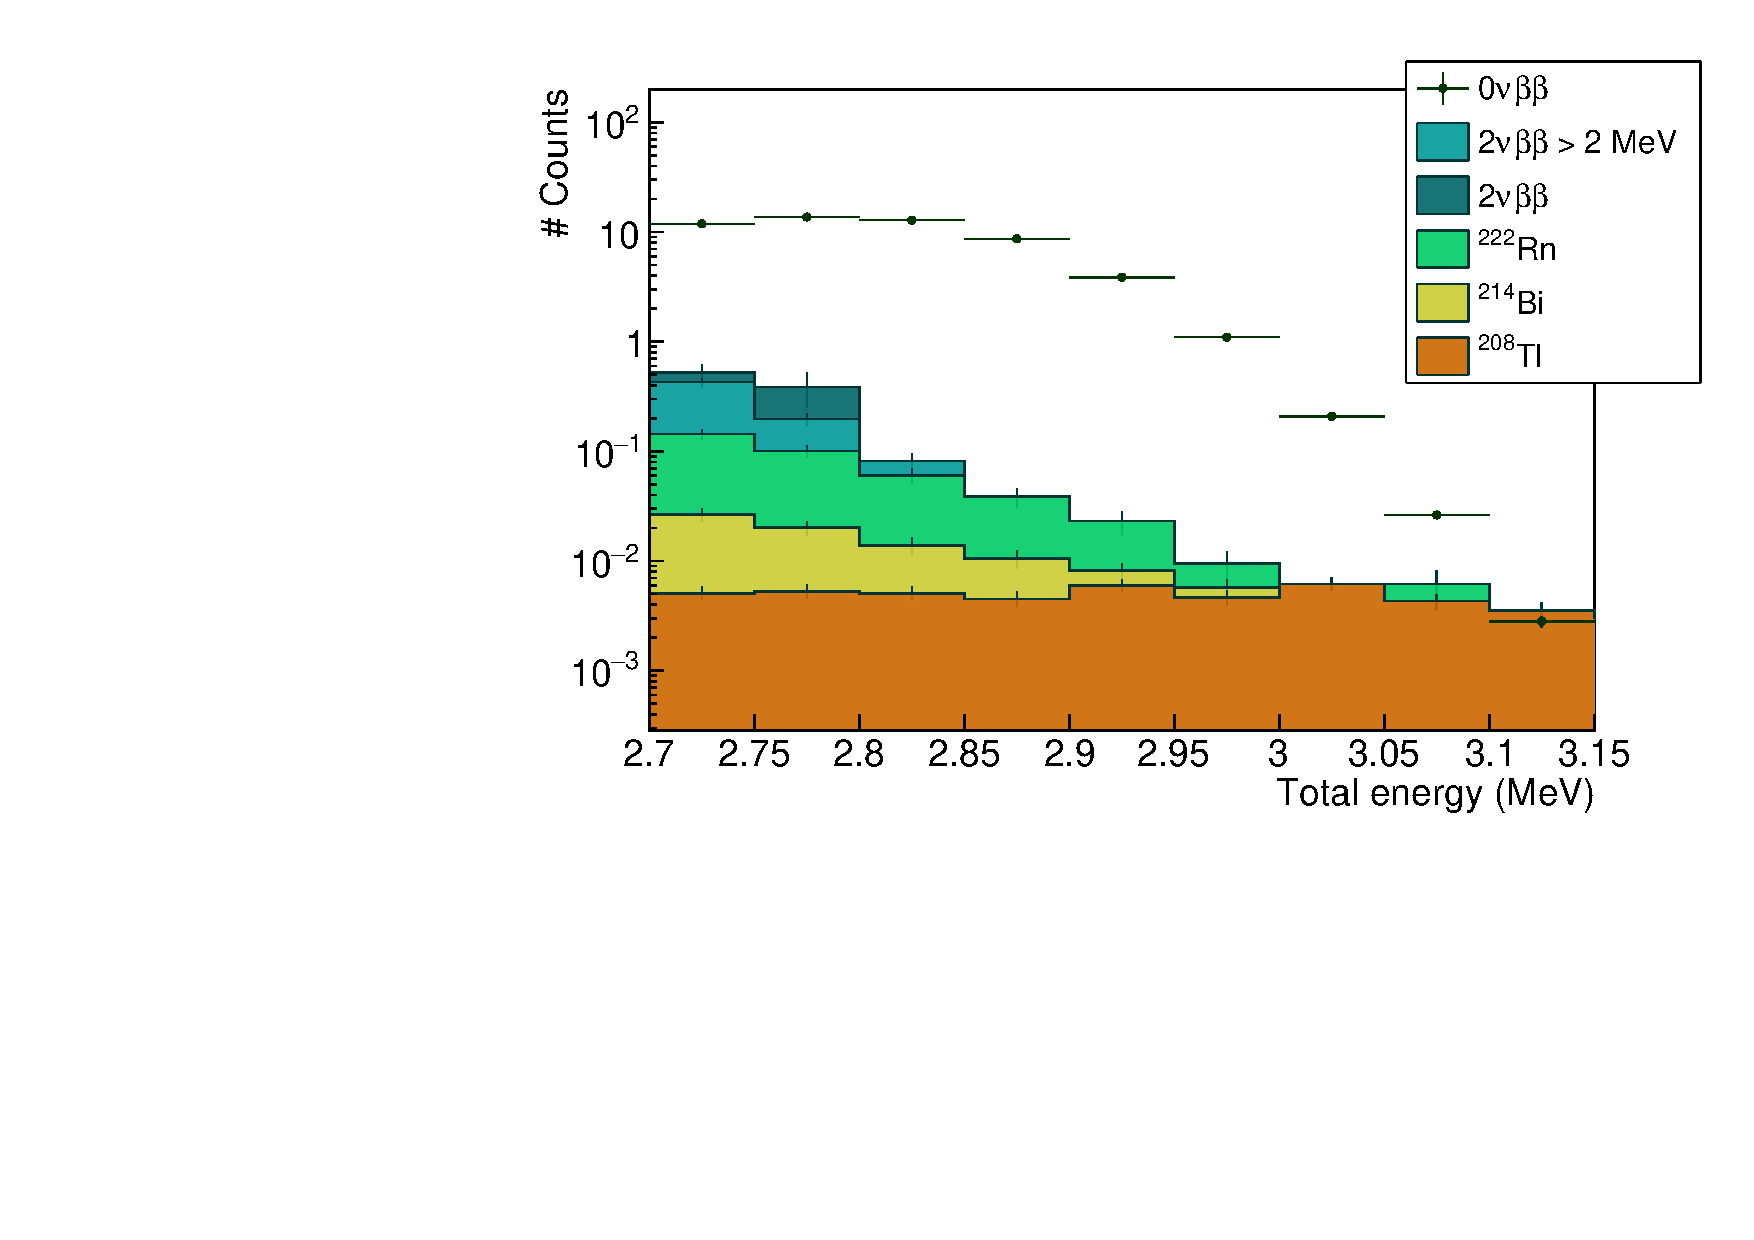
\includegraphics[width=1.1\textwidth]{Sensitivity/fig_sensitivity/energy_spectrum_with_B_82Se_zoom.pdf}
  \captionsetup{justification=centering}
  \caption{Zoom on ROI.
    \label{subfig:energy_spectra_zoom}}
\end{subfigure}
\caption{Total energy spectra for the $\zeronu$ signal and main backgrounds, for (a) the full energy range, and (b) for the [$2.7$;$3.15$]~MeV energy range, whose optimisation is discussed in Sec.~\ref{sec:Nbkg_ROI}.
  The $\twonu$ spectrum is normalised to $\Ttwonu~=~9.39\times~10^{19}$~y, and the specified activities are considered for \Tl,\Bi\ and \Rn.
  The amplitude of the $\zeronu$ is arbitrarily set at the limit obtained with NEMO-$3$.
  \label{fig:energy_spectra}}
\end{figure}
The distributions are given for the demonstrator (\Se\ sources, $17.5$~kg.y exposure), considering the specified activities are reached.
If the $\zeronu$ decay is detected, the two-electrons energy sum distribution would be a peak, located at the end-point of the $\twonu$ energy distribution, that is to say at the total available energy, $\Qbb = 2.99$~MeV.
As the two electrons of this decay would share the total available energy, this peak should be infinitely thin.
However, a widening of this distribution is expected, due to energy losses inside the dense source material.
Indeed, the path of an electron in the source is more or less long, depending on the disintegration location and on the emission angle, leading to a degradation of the measured energy.
This peak is also expected to be shifted towards small energies, by the calorimeter energy resolution and the straggling of energy losses inside the wire chamber.
Consequently, the $\zeronu$ energy distribution is expected to be asymmetrical, as displayed in the figure.

As explained in Sec.~\ref{sec:sensitivity_simus}, two sets of $\twonu$ events were simulated: one on the full energy range, and one for which the two-electrons energy sum is greater than $2$~MeV.
After the normalisation of these two sets, we get the complete $\twonu$ energy spectrum displayed in the figure.
The \Tl\ total energy spectrum extends up to high energies.
  It reveals two distinct peaks, one corresponding to a low-energy $\beta$ particle, the other to the internal conversion of the $2.614$~MeV gamma, emitted after \Tl\ $\beta^{-}$ disintegrations (Sec.~\ref{subsec:SNbkg_internal}).
Whatever their origin, either \Rn\ contaminations inside the tracker gas, or internal contaminations of the source foils, the two \Bi\ energy distributions have nearly the same shapes.

% The progeny of \Rn\ produces $\gamma$-rays and $\beta$ decays accompanied by internal conversion (IC), Møller or Compton scattering, the dominant mechanism being the first one.
%%Therefore, given the activities of \Rn\ in the tracker and \Bi\ inside the source foils, theses two background types both contribute at the same level in the full energy range.
These energy spectra confirm the $\twonu$ background is dominant in the total energy range.
Therefore, a widespread technique consists in constraining the $\zeronu$ decay searches to a narrow energy range, the so-called \emph{region of interest} (ROI).
It allows to reduce the total number background decays, while maximising the chances of observing the signal decay, then to maximise the limit set on $\Tbeta$.
A typical ROI is materialised in the figure by two vertical dashed lines, revealing \Tl, \Bi\ and \Rn\ could be harmful for the search for the $\zeronu$ decay.
The influence of the sources contamination by these natural isotopes, as well as optimised background rejection techniques are presented in Sec.~\ref{sec:demonstrator_sensitivity}.

In the following, we expose general principles leading to the determination of the best limit on $\Tbeta$, in the appropriate region of interest.
We illustrate the reasoning by applying it on the demonstrator case, with specified activities, and on-magnetic field condition.
However, the technique presented remain valid for all exposures, internal contamination levels and field conditions.


\section{Demonstrator sensitivity to the $\zeronu$ decay of \Se}
\label{sec:Nbkg_ROI}

The SuperNEMO demonstrator is designed to measure $\beta\beta$ decays of radioactive emitters.
In case a the non-observation of the $\zeronu$ process, the collaboration would set an lower-limit on the half-life $\Tbeta$, and an upper-limit on the effective neutrino mass $\mbb$.

\subsection{Sensitivity to the $\zeronu$ half-life}

In case of the non-observation of a $\zeronu$ signal, the expected lower limit on the half-life is provided for a given energy range [$E_{\text{min}}$;$E_{\text{max}}$] on the two electrons energy sum, and depends on the characteristics of the detector.
Firstly, it depends on the signal detection efficiency, $\epsilon_{0\nu}$ in this energy window, which corresponds to the ratio of the number of selected signal events to the number of simulated ones.
It also depends on the source isotope nature, as well as on the detector exposure $m\times t$, with $m$ the mass of source material in the foils and $t$ the data acquisition time period.
It follows
\begin{equation}
  \Tbeta > \frac{\mathcal{N}_{\text{A}}\ln{2}}{M}\times \frac{\epsilon_{0\nu}\times m\times t}{N_{0\nu}^{\text{excl.}}}\,,
  \label{eq:tbeta_limit}
\end{equation}
with $\mathcal{N}_{\text{A}}$ the Avogadro number and $M$ the $\beta\beta$ emitter molar mass.
$N_{0\nu}^{\text{excl.}}$ is the number of signal events excluded at a given confidence level (usually $90$\%), calculated with the Feldman-Cousins statistics from the total expected number of background events.
The Feldman-Cousins statistics~\cite{art:feld-cous} is a wide-used method in rare events search experiments, providing confidence intervals for upper limits in the case of background events following a Poissonian probability law.
We use this method in the framework of this analysis to provide a limit, at $90\%$ CL, on the number of excluded signal events $N_{0\nu}^{\text{excl.}}$, on the basis of the expected number of background events, given below.
\begin{itemize}
\item The $\twonu$ background\\
  Eq.~\eqref{eq:tbeta_limit} defines the lower limit on $\Tbeta$ from the number of excluded signal events, and the signal selection efficiency $\epsilon_{0\nu}$.
  In a similar manner, we can define the number of expected $\twonu$ events, $N_{2\nu}$, from the half-life $\Ttwonu$ and the $\twonu$ selection efficiency, $\epsilon_{2\nu}$, as
  \begin{equation}
    N_{2\nu} = \frac{\mathcal{N}_{\text{A}}\ln{2}}{M}\times\frac{\epsilon_{2\nu}\times m\times t}{\Ttwonu}\,.
    \label{eq:N_2nu}
  \end{equation}
\item Natural radioactive backgrounds\\
  We consider the background massic activities $A_{\text{rad.}}$, and $\epsilon_{\text{rad.}}$ their selection efficiencies in a given energy window.
  The number of background events is therefore given, for the \Tl\ and \Bi\ internal contaminations, as
  \begin{equation}
    N_{\text{rad.}}^{m} = A_{\text{rad.}}^{m}\epsilon_{\text{rad.}}^{m}\times m\times t\,,
  \end{equation}
  where $A_{\text{rad.}}$ is given in Bq/kg.
  Similarly, for the \Rn\ background,
  \begin{equation}
    N_{\text{rad.}}^{V} = A_{\text{rad.}}^{V}\epsilon_{\text{rad.}}^{V}\times V\times t\,,
    \label{eq:N_Rn}
  \end{equation}
  with $V = 15.3$ m$^{3}$ the total tracker volume, and $A_{\text{rad.}}$ represents here a volumic activity, given in Bq/m$^{3}$.
\end{itemize}

As we said, all equations from Eq.~\eqref{eq:tbeta_limit}~to~\eqref{eq:N_Rn}, are valid for a given energy range [$E_{\text{min}}$;$E_{\text{max}}$].
To find the optimal energy interval for the search for the $\zeronu$ decay, that is to say the one maximising the limit on $\Tbeta$, we must study the influence of the variations of E$_{\text{min}}$ and E$_{\text{max}}$ bounds on the final sensitivity.
On Fig.~\ref{fig:energy_spectra}, we observe that beyond the energy sum of $3$~MeV, the total number of background events is highly reduced, and the \Tl\ background dominates, with $0.03$ count expected for E$>3.2$~MeV.
This is why the upper limit E$_{\text{max}}$ of the energy interval has only a limited impact on the search for the best ROI.
It is then natural to study mainly the influence of the lower limit E$_{\text{min}}$.
In that purpose, the selection efficiencies, entering in the calculation of the $\Tbeta$ lower limit, are presented in Fig.~\ref{fig:efficiency_spectra}, as a function of the lower bound $\text{E}_{\text{min}}$.
\begin{figure}[h!]
  \centering
  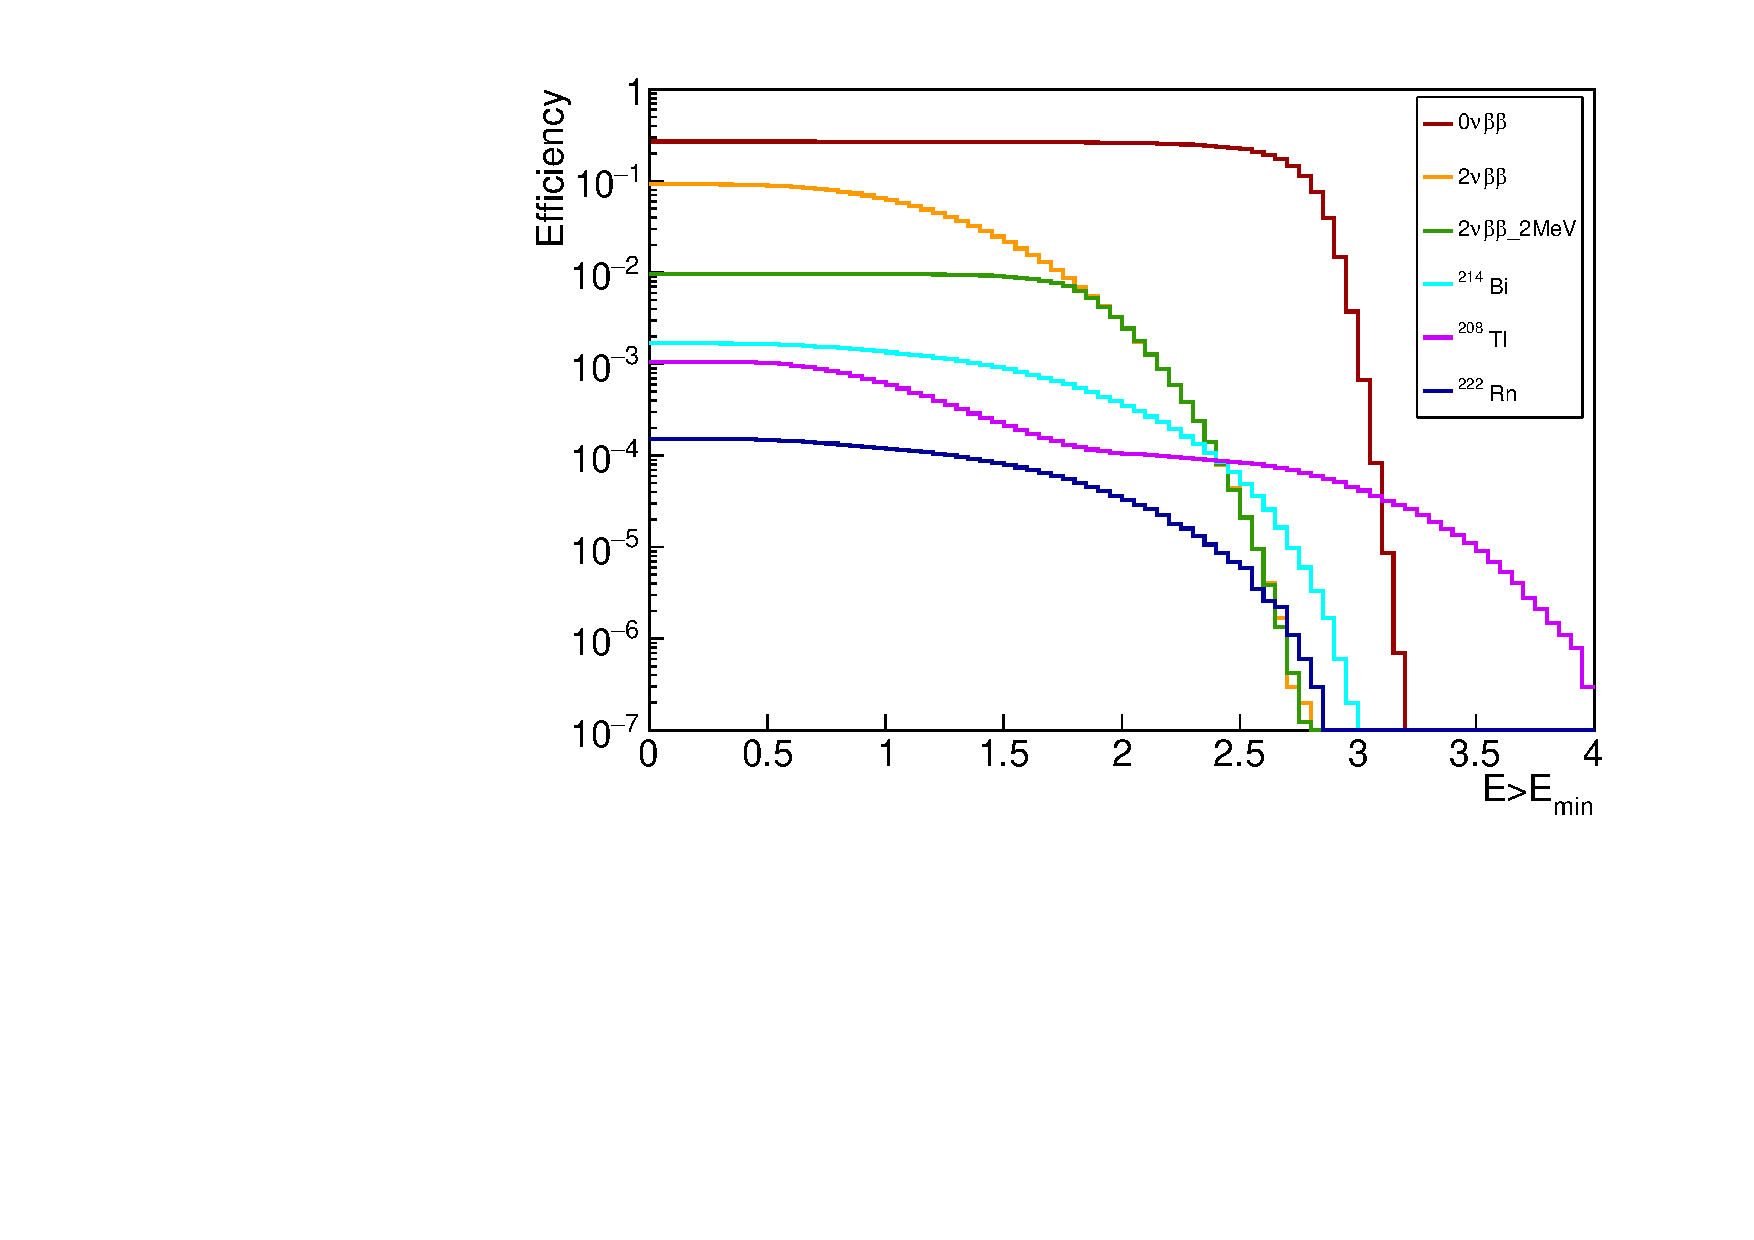
\includegraphics[width=0.8\textwidth]{Sensitivity/fig_sensitivity/efficiency_spectrum_with_B_82Se.pdf}
  \caption{Efficiency spectra as a function of $\text{E}>\text{E}_{\text{min}}$, for the $\zeronu$ signal (dashed black line) and for the main backgrounds (plain lines).
    The two vertical grey lines depict the final ROI optimised for the case of the demonstrator, taken the specified isotope activities.
    \label{fig:efficiency_spectra}}
\end{figure}
As a matter of fact, the ROI would correspond to an energy range where $\epsilon_{0\nu}$ is high, and where selection efficiencies for the background are low, in order to maximise the $\Tbeta$.
The variations of the limit set on $\Tbeta$ (at $90$~\% CL) as a function of E$_{\text{min}}$ and E$_{\text{max}}$ are presented in Fig.~\ref{fig:sensitivity_cont}.
\begin{figure}[h!]
  \centering
  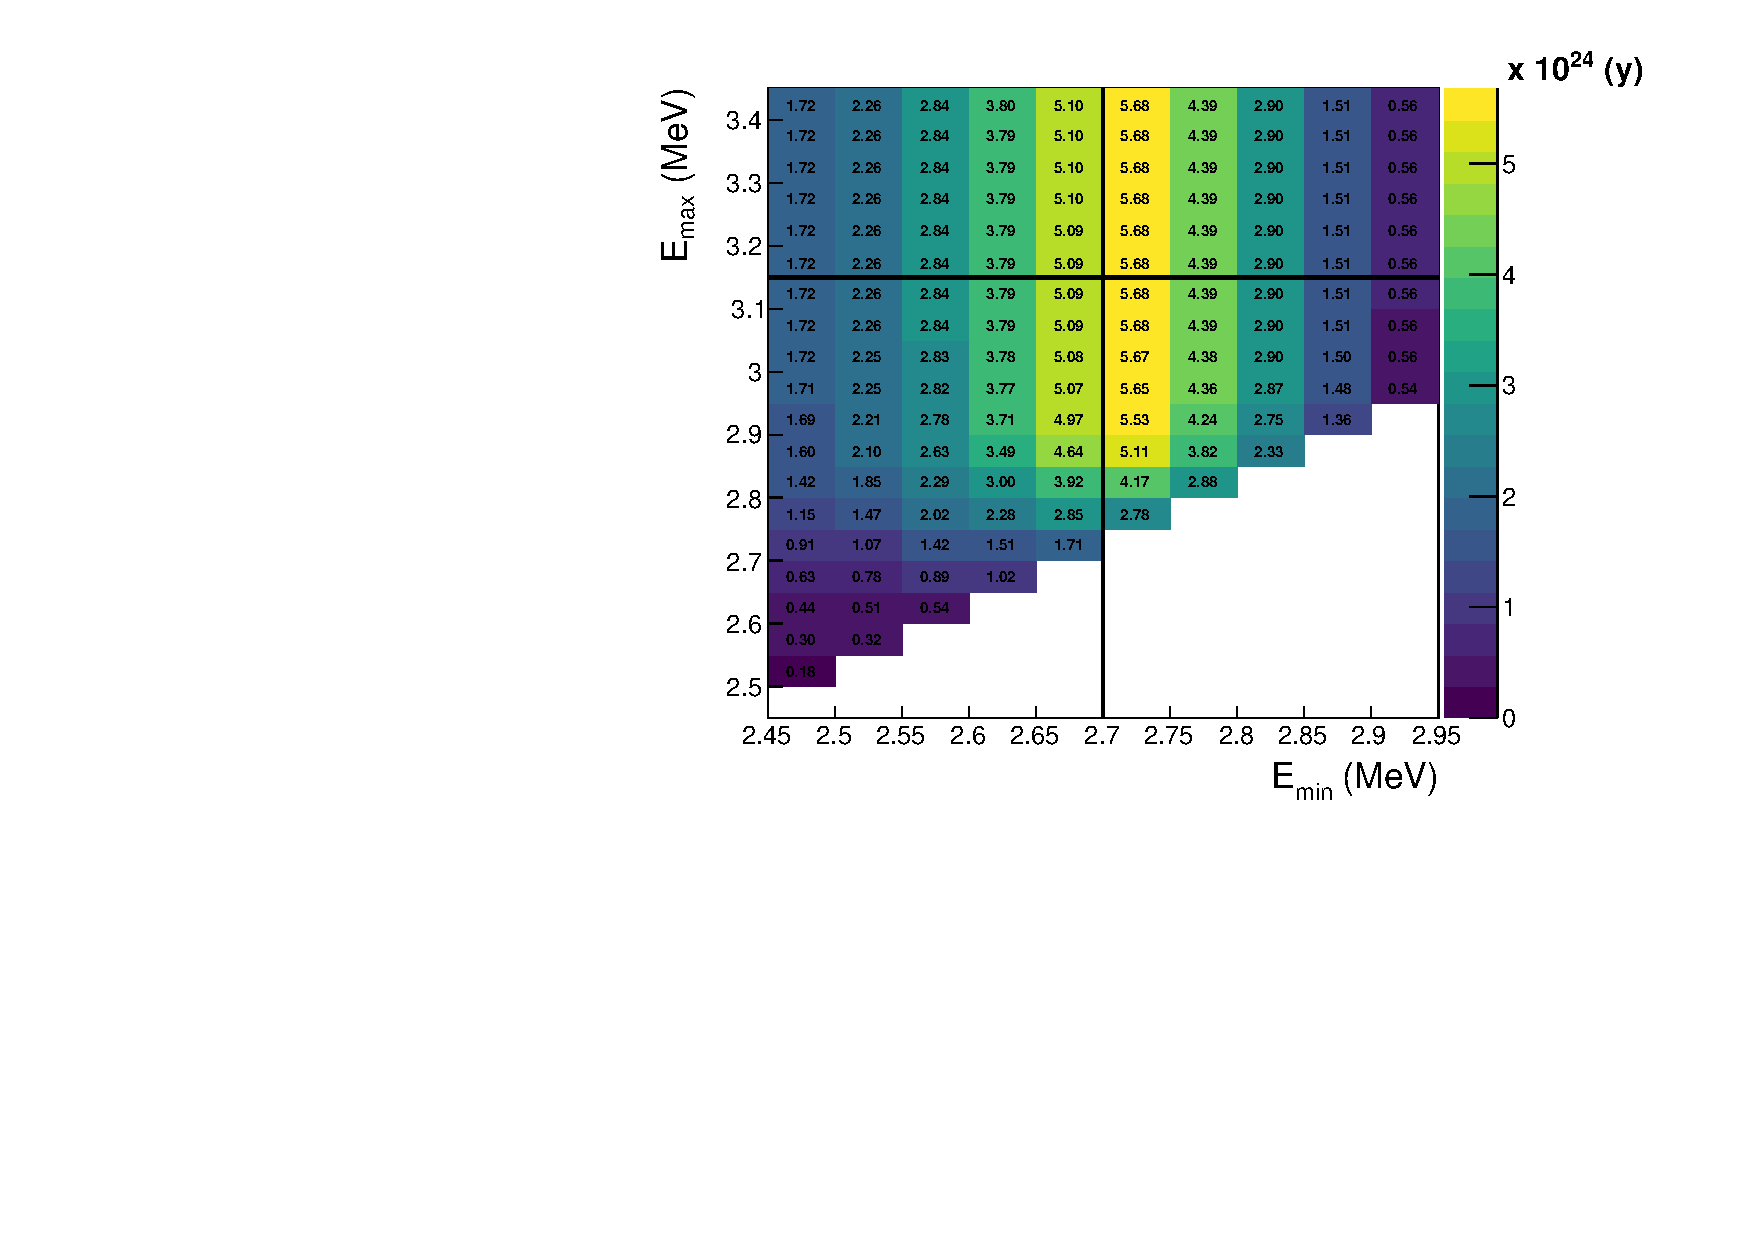
\includegraphics[width=1.1\textwidth]{Sensitivity/fig_sensitivity/sensitivity_spectrum_with_B_82Se.pdf}
  \caption{Two-dimensional histogram showing the evolution of the $\Tbeta$ $909$\% limit as a function of the lower and upper energy bounds.
    The maximal lower limit of $\Tbeta~>~5.7\times~10^{24}$~y (90\%~CL) is retained, in the [$2.7$;$3.15$]~MeV region of interest.
    \label{fig:sensitivity_cont}}
\end{figure}
We found that, for the demonstrator exposure, with \Se\ sources, with a $25$ Gauss magnetic field, and for the specified background activities, the best ROI is [$2.7$;$3.15$]~MeV.
As expected, as long as the upper bound is larger than $3.15$~MeV, the sensitivity on the search for $\zeronu$ is not affected.
Therefore, this value is kept in order to enter into a future more general study, taking into account the neutron background of the experiment, which extends at high energies.
Tab.~\ref{tab:eff_nominal_ROI} summarises the expected number of background events for each non-zero contamination case presented in Fig.~\ref{fig:real_target_act}.
\begin{table}[h!]
  \centering
  \begin{tabular}{|c|c|}
    \hline
    Process & Event selection \\
    \hline\hline
    $\epsilon_{0\nu}$ & $14.7$\% \\
    \hdashline
    $\twonu$  & $0.418$ \\
    \Tl  & $0.0475$  \\
    \Bi  & $0.0546$   \\
    \Rn  & $0.292$  \\
    Total & $0.394$ \\
    \hline
  \end{tabular}
  \caption{Selection efficiency of $\zeronu$ events and expected number of backgrounds events in the optimised ROI [$2.7$;$3.15$]~MeV, for the exposure of the SuperNEMO demonstrator (17.5 kg.y).
    The specified levels of contamination are considered.
    \label{tab:eff_nominal_ROI}}
\end{table}



In the optimised [$2.7$;$3.15$]~MeV energy range, the sensitivity expected for the SuperNEMO demonstrator stands at
\begin{equation}
\Tbeta > 5.7\times 10^{24}\,\text{y}\qquad (90\% \text{CL})\,.
\end{equation}
This result is compatible with previous SuperNEMO analysis~\cite{CalvezThesis}.


\subsection{Limit on the effective neutrino mass}

The decay rate for the light Majorana exchange mechanism is given by:
\begin{equation}
  (T_{1/2}^{0\nu})^{-1} = g_{A}^{4}G^{0\nu}|M^{0\nu}|^{2}\left\lvert\dfrac{m_{\beta\beta}}{m_{e}}\right\rvert^{2}\,.
\end{equation}
where $G^{0\nu}$ is the two particles phase space factors, depending on $\Qbb$ and Z the number of protons, $M^{0\nu}$ is the nuclear matrix elements for the $\zeronu$ process, and $\mbb$ is the effective Majorana neutrino mass, defined as
\begin{equation}
  \langle \mbb \rangle = \left\vert \Sigma_{i}m_{i}U^{2}_{ei} \right\vert \,,
\end{equation}
where $m_{i}$ are the neutrino masses, and $U^{2}_{ei}$ is the mixing matrix.
Therefore, the effective mass takes into account the neutrino mixing.
Consequently, observing the $\zeronu$ decay would not only prove the Majorana nature of neutrinos but, assuming the mass mechanism, could also help constraining the absolute neutrino masses.
Given $g_{A}$, $G^{0\nu}$ and $M^{0\nu}$~\cite{PhysRevC.85.034316,PhysRevC.83.034320}, we find the SuperNEMO demonstrator could reach a limit on the effective neutrino mass of
\begin{equation}
\langle\mbb\rangle < [0.24-0.47]~\text{eV}\qquad (90\% \text{CL})\,.
\end{equation}
Although this limit is not competitive with other current $\zeronu$ experiments, this is an improvement compared to NEMO-$3$, demonstrating that SuperNEMO's technology would benefit from being adapted to larger scales.

In this section, we presented the general procedure leading to an optimised result on the $\Tbeta$ limit, and gave a result for the SuperNEMO demonstrator compatible with the previous studies led by the collaboration.
Thereafter, we discuss the results obtained for different detector exposures (demonstrator and final detector), and different internal background activities.
Also, and this is the main purpose of this study, we discuss the influence of the presence of the magnetic field on the final detector's sensitivity.
%%


\section{Impact of sources contamination levels on the sensitivity}
\label{sec:demonstrator_sensitivity}

We study the impact of the isotope contamination levels (inside the source foils, as well as on the tracker's wires) on the $\zeronu$ sensitivity.
We also optimise additional event selections aimed at improving it.


\subsection{Contamination levels}
\label{subsec:Influence_cont}

Strict specifications have been defined for source foil contamination in order to achieve the target sensitivity for the final SuperNEMO detector ($500$~kg.y).
BiPo detector and SuperNEMO collaboration measurements (Sec.~\ref{subsec:SNbkg_internal}) have shown that the \Tl\ level is not reached for the demonstrator source foils, being almost $27$ times higher than expected, with $\mathcal{A}^{\text{Tl}}~=~54~\mu$Bq/kg [$26$~-~$102$].
Also, the \Bi\ contamination is not greater than $290\,\mu$Bq/kg at $90$\% CL.
If this upper limit was reached we would expect $1.6\times~10^{5}$ internal Bismuth events in the total energy range.
Fortunately, the Radon contamination inside the wire chamber does not exceed the specifications supposing an gas flow  rate of $2$~m$^{3}$/h inside the chamber.
In Sec.~\ref{sec:Nbkg_ROI}, we developed the general procedure allowing to set a $90\%$ confidence interval limit on $\Tbeta$.
For the demonstrator, supposing the specified activities are reached, the demonstrator would achieve a sensitivity of $5.7\times~10^{24}$~years on the searched decay, in $2.5$~years of data acquisition, with $7$~kg of \Se.
This sensitivity could be affected by the higher-than-specified levels of internal contaminations measured by BiPo.

%% For each level, we oppose two distinct magnetic field cases: a $25$~G magnetic field, or no field.
%% In the current sub-section, we focus on the comparison between different contamination levels.
%% The conclusions about the presence of the magnetic field we will be discussed in the next sub-section.
In this sub-section, four distinct levels of internal contaminations are considered:
\begin{itemize}
\item the \emph{zero activities} case, a hypothetical case where the source foils and the tracker are non contaminated at all by natural isotopes,
\item the \emph{specified activities} case, where the targeted level of contaminations would have been reached,
\item and two \emph{measured} cases.
  As the \Bi\ activity is provided by BiPo measurements as an upper limit, we choose to present the results either for sources that would not be contaminated by this isotope (the \emph{without \Bi} case), or considering that the activity reached is $290\,\mu$Bq/kg (\emph{with \Bi}).
  The \Tl\ activity considered for these two measured cases is the limit at $90$\% CL.
\end{itemize}
The fact that we are showing results for a hypothetical zero isotope contamination is to illustrate an important phenomenon about the Feldman-Cousins statistics employed to determine the number of excluded signal events, $N_{0\nu}^{\text{excl.}}$, given the number of observed background events (defined from Eq.~\eqref{eq:N_2nu} to Eq.~\eqref{eq:N_Rn}).

\paragraph{Clarifications on Feldman-Cousins statistics}
When the expected number of background events is negligible (which is the case for the zero and specified levels), the probability $p$ to observe $n_{s}$ signal events, expecting $s$ events, is given by the Poisson distribution
\begin{equation}
p = \frac{e^{-s}s^{n_{s}}}{n_{s}!}\,.
\end{equation}
Let's now put ourselves in the situation where no signal event is observed - that is what we assume to put an lower limit on the $\zeronu$ half-life.
Then $n_{s}\rightarrow~0$, and $p\rightarrow~e^{-s}$.
If zero signal event is \emph{observed}, it is incorrect to assume that zero signal events were \emph{produced} during the experiment.
We only can say that no signal event has been observed \emph{a priori}.
To account for this particular case, the quantity $s$ should no longer be viewed as the number of expected signal events, but as the number of excluded signal events, $N_{0\nu}^{\text{excl.}}$.
In the end, for a negligible expected number of background events, and no signal event observed, we can set an lower limit on the number of excluded signal events, excluding values for which $p < \alpha$.
Taking a $90\%$ confidence interval, that is to say $\alpha~=~10\%$, we obtain $s \leq 2.303$.

\paragraph{} We show in Fig.~\ref{fig:real_target_act} the $90$~\%~CL $\Tbeta$ limit for the four contamination levels considered, as well as the corresponding regions of interest, optimised following the technique explained in Sec.~\ref{sec:Nbkg_ROI}..
\begin{figure}[h!]
  \centering
  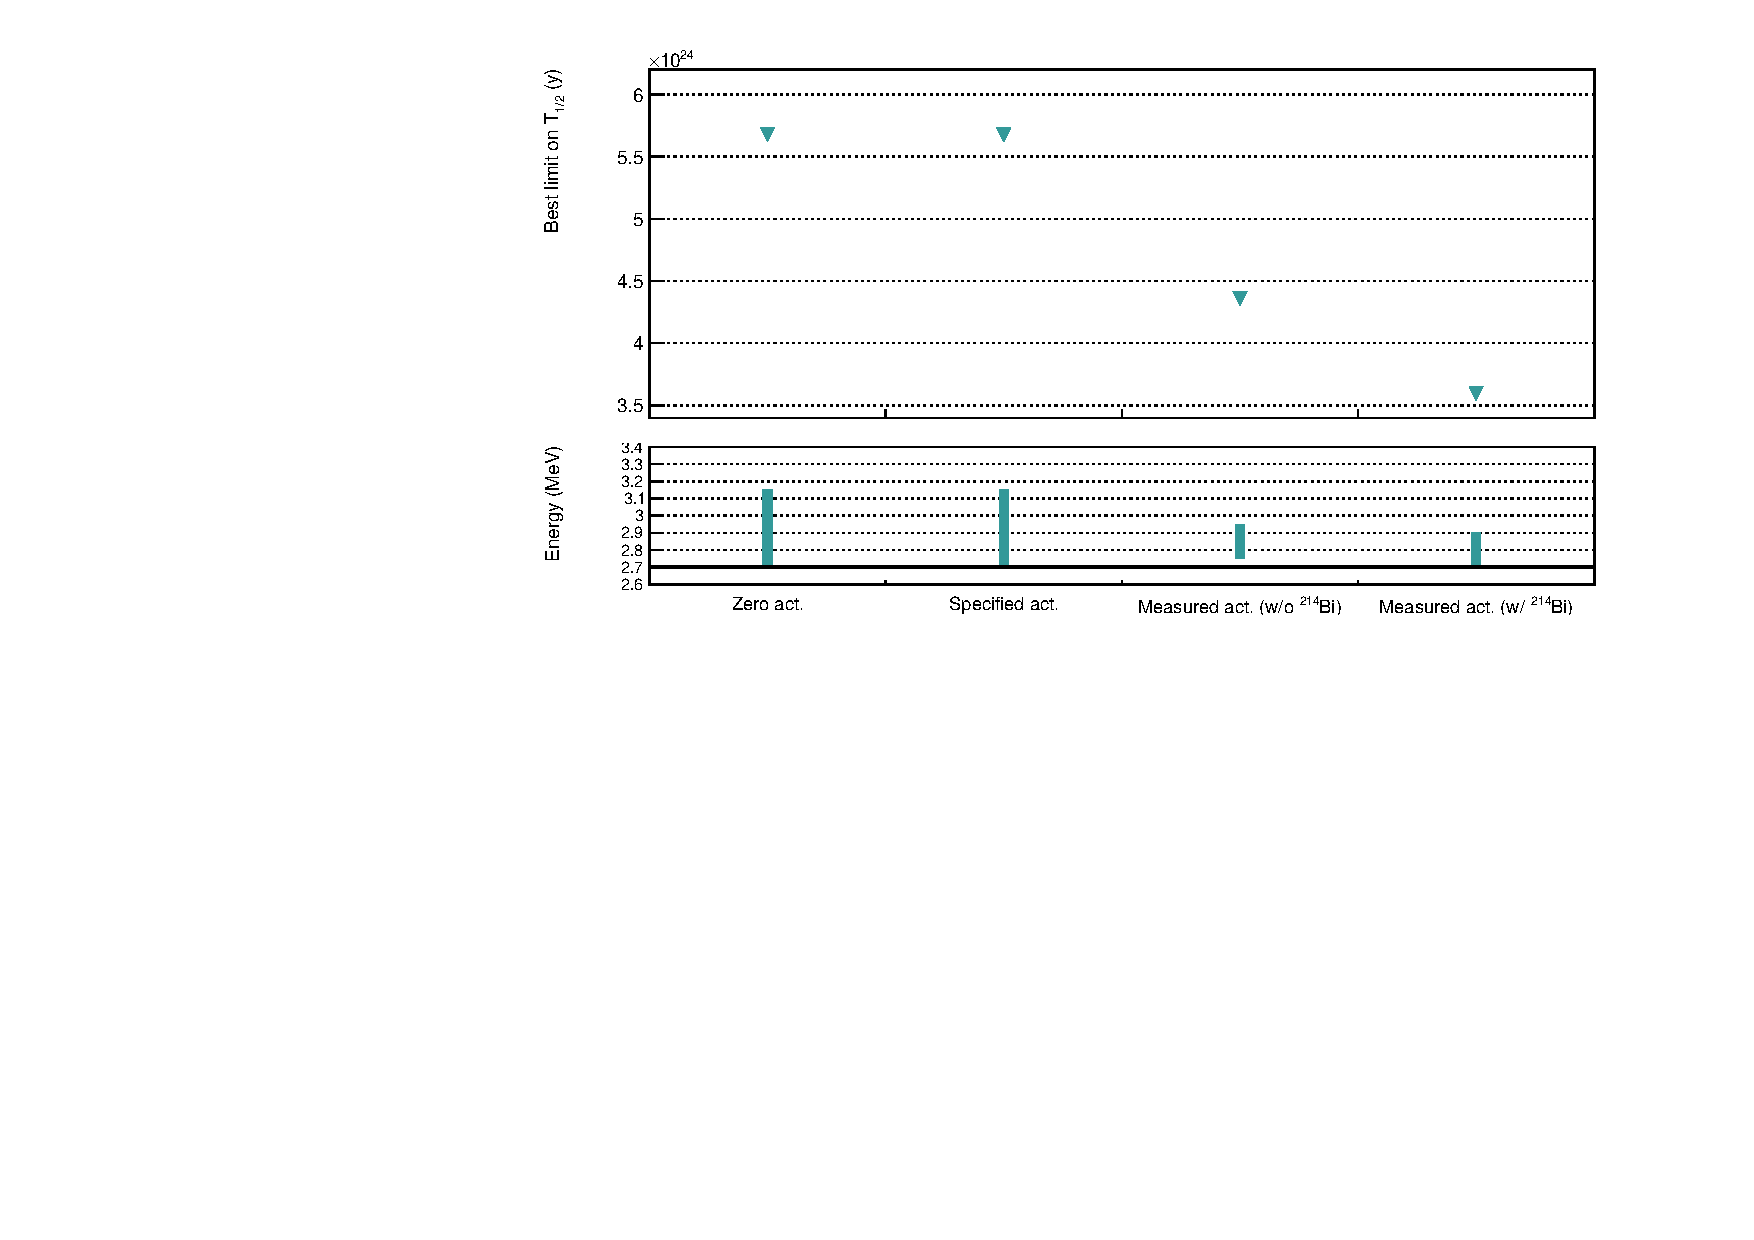
\includegraphics[width=1.1\textwidth]{Sensitivity/fig_sensitivity/contamination_level_Se_B.pdf}
  \caption{The $90\%$ CL limit on the $\zeronu$ half-life (top pad), and the corresponding ROI (bottom pad), as a function of the contamination level considered.
    For the \emph{zero activities} case, we consider hypothetical contamination levels where $\mathcal{A}^{\text{Bi}}~=~\mathcal{A}^{\text{Tl}}~=~0~$Bq/kg.
    The \emph{specified activities} are presented in Tab.~\ref{tab:real_target_act}.
    The \emph{measured activities}, provided by the BiPo detector~\cite{internal:bipo}, are presented in the same table.
    We consider successively a null \Bi\ contamination (\emph{measured act. w/o \Bi}), or equals to the $290\mu\,$Bq/kg upper limit (\emph{measured act. w/ \Bi}).
    \label{fig:real_target_act}}
\end{figure}
As expected from the previous conclusions given on the Feldman-Cousins statistics, no difference is observed in terms of half-life limits, or ROI, between the zero and specified activity cases.
Now considering the two measured activity cases, the sensitivity is decreased compared with the specified case.
Indeed, the number of background events in the ROI is no more negligible, and influence significantly the value of $\Tbeta$, decreasing the experiment's sensitivity by $23\%$ (without \Bi) and $37\%$ (with \Bi).
%% To help visualise the situation, we show in Fig.~\ref{} the distribution of $N_{0\nu}^{\text{excl.}}$, for the demonstrator case, for the two first contamination cases.
%% \begin{figure}[h!]
%%   \centering
%%   \includegraphics[width=1.1\textwidth]{Sensitivity/fig_sensitivity/}
%%   \caption{
%%     \label{fig:}}
%% \end{figure}

Tab.~\ref{tab:eff_first_order_contamination} summarises the expected number of background events for each non-zero contamination case presented in Fig.~\ref{fig:real_target_act}.
\begin{table}[h!]
  \centering
  \begin{tabular}{|c|c|c|c|}
    \hline
    Activity & Specified & Measured (w/o \Bi) & Measured (w/ \Bi) \\
    ROI & [$2.7$;$3.15$]~MeV & [$2.75$;$2.95$]~MeV & [$2.7$;$2.9$]~MeV \\
    \hline\hline
    $\epsilon_{0\nu}$ & $14.7$\% & $11.3$\% & $14.3$\% \\
    \hdashline
    $\twonu$  & $0.418$ & $0.122$ & $0.418$ \\
    \Tl  & $0.0475$ & $0.688$ & $0.699$ \\
    \Bi  & $0.0546$ & $0$ & $1.55$ \\
    \Rn  & $0.292$ & $0.173$ & $0.287$ \\
    Total & $0.812$ & $0.983$ & $2.95$ \\
    \hline
  \end{tabular}
  \caption{Selection efficiency of $\zeronu$ events and expected number of backgrounds events in the optimised ROI, for the exposure of the SuperNEMO demonstrator (17.5 kg.y).
    Three levels of contamination are considered.
    \label{tab:eff_first_order_contamination}}
\end{table}
Regions of interest, optimised for each activity, are reminded.
The total number of background events for the specified activity case is negligible in this region.
This is the reason why the limit of $2.303$ on the number of excluded signal events is reached, according to the statement made on Feldman-Cousins statistics.
For the two measured activity cases, the expected number of background events increases significantly, explaining the degradation of the sensitivity.
Hopefully, both regions of interest are highly reduced, especially for the case without \Bi, where the lower bound is increased from $2.7$ to $2.75$~MeV.
As this $50$~keV wide energy region is populated with a non-negligible number of background events, this change in $\text{E}_{\text{min}}$ usefully reduces the $\twonu$ background contribution, thereby limiting the increase of total expected number of background.

The degradation of the limit on the $\zeronu$ half-life with the level of contamination remains acceptable.
However, we can try improving the situation by exploring new background rejection techniques.
This would be especially useful for the final detector case, where a slight increase in internal contaminations could be highly harmful, all the more so as the upper limit given for \Bi\ turns out to be the true contamination level.

\subsection{Optimisation of event selection}
\label{subsec:opti_ev_selection}

%% The measured level of \Tl\ isotope inside the source foils is greater than the specifications.
%% Moreover, an upper limit, higher than the specified level for SuperNEMO, has been set by the BiPo detector, regarding the internal \Bi\ level.
Following the BiPo radiopurity measurements, we wish to implement additional event selections, to reject a higher quantity of background.
Most of the double beta experiments are only sensitive to the total electron energy sum.
The unique SuperNEMO tracko-calo technology confers the experiment the ability to characterise single particles (individual energies, emission angles...).
Based on previous studies~\cite{CalvezThesis,ChaponThesis}, \emph{topological cuts}, relying on these additional observables, can be set up.
They are especially designed to reject events where the two electrons are not emitted simultaneously, or from the same location on the source foils.

\subsubsection{The internal probability}
Based on time-of-flight (TOF) computation, the internal probability (\Pint) is derived from the internal $\chi^{2}_{int}$ (see details in Sec.~\ref{subsec:internal_prob}).
In Fig.~\ref{fig:Pint} are presented the internal probability spectra for the $\zeronu$ signal and all background processes, after the first-order selections.
\begin{figure}[h!]
  \centering
  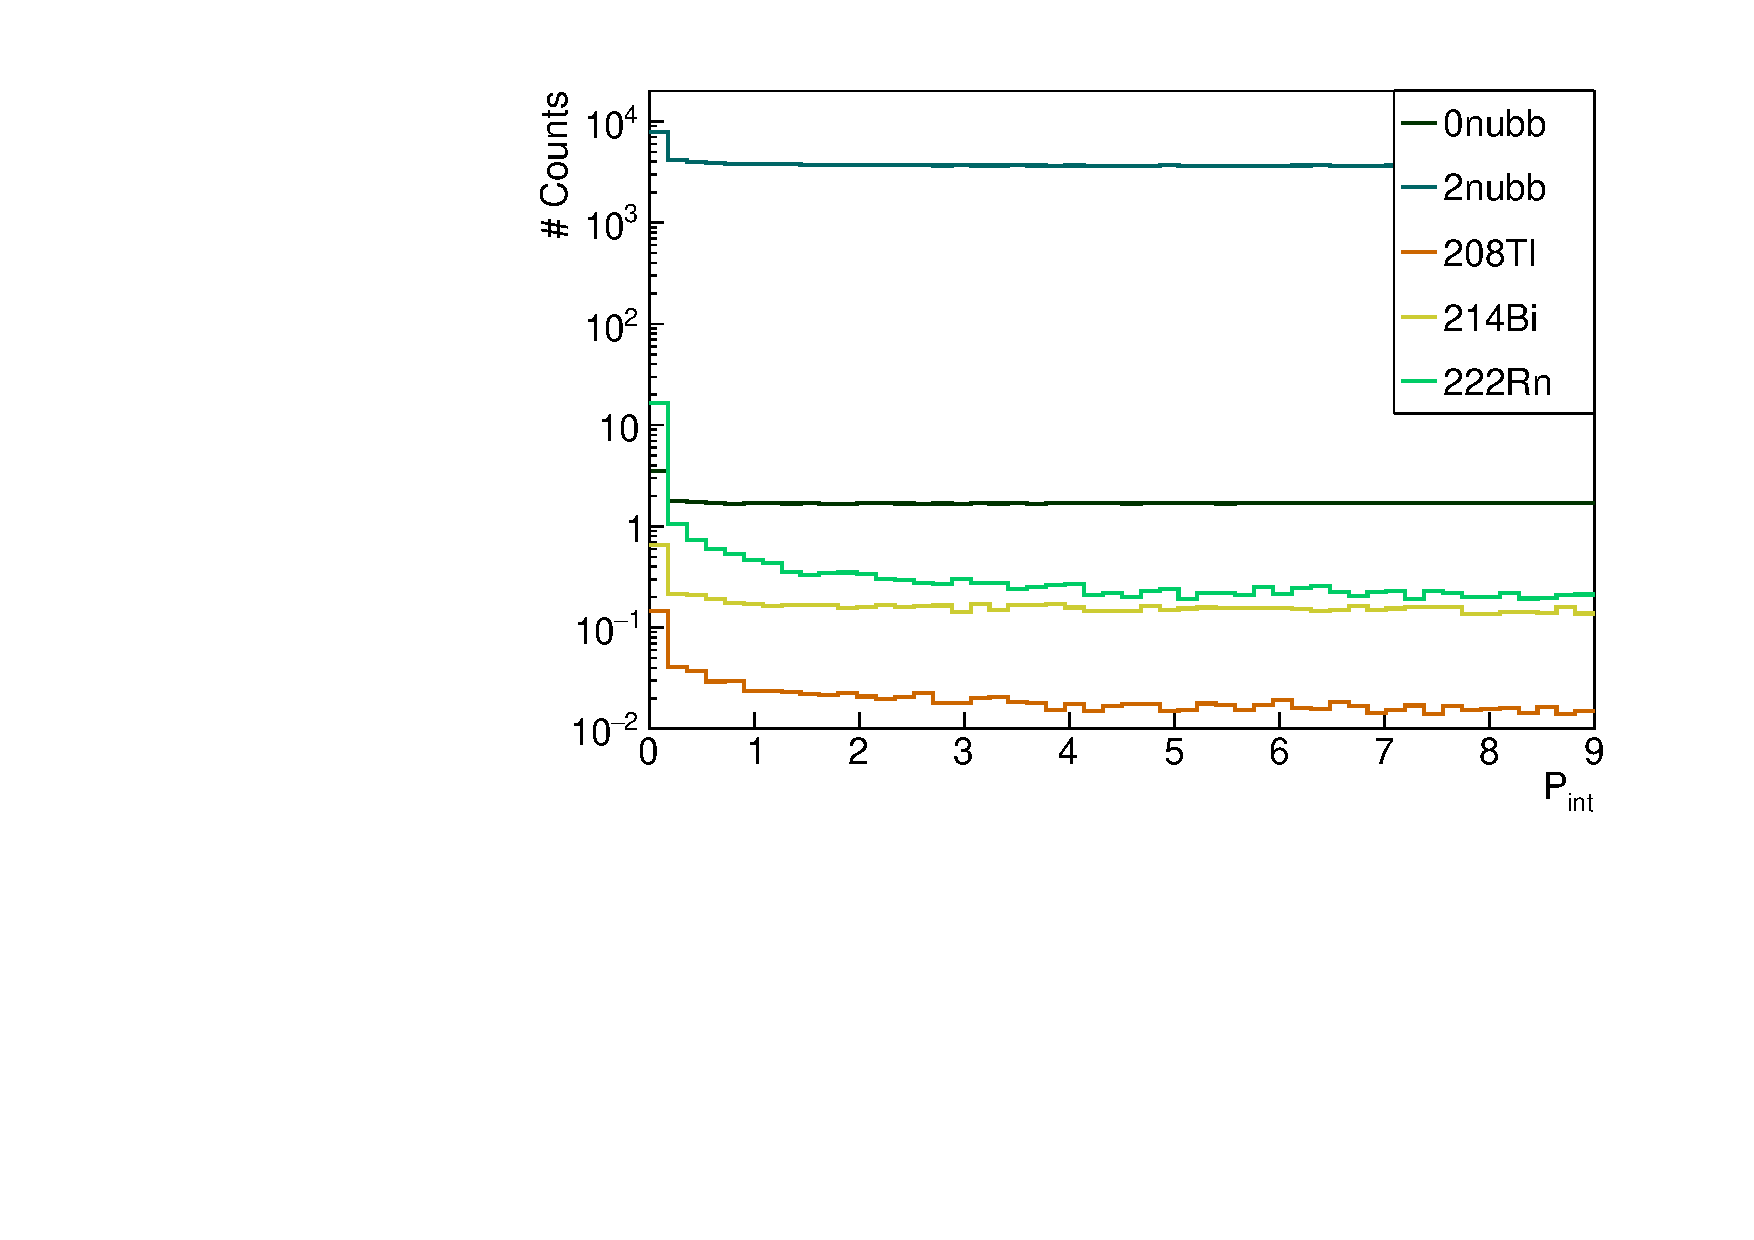
\includegraphics[width=0.8\textwidth]{Sensitivity/fig_sensitivity/InternalProbability.pdf}
  \caption{Internal probabilities for all processes.
    First-order cuts have been applied.
    $\beta\beta$ distributions are normalised to the half-lives, and background processes are normalised to the specified activities.
    \label{fig:Pint}}
\end{figure}
These distributions are normalised to the double beta half-lives, and the nominal activities.
Equivalent distributions, but with different \Bi\ and \Tl\ contamination levels, can be derived for the case of measured activities.
The internal probability distributions for the $\zeronu$ and $\twonu$ processes follow the expected flat distribution for electrons emitted simultaneously from the source.
As internal Bismuth disintegration actually takes place inside the sources, the \Bi\ distribution is also flat.
The same could have been assumed for Thallium, however, the distribution is distorted at low internal probabilities.
This might be explained by the existence of a metastable excited state ($\tau_{1/2} = 294 ps$) of the daughter nuclei, which would slightly delay the second electron emitted via internal conversion.
This feature is addressed in detail in Chap.~\ref{ch:timediff}.
The Radon, being a non-internal background, presents a large peak at low internal probabilities.

We want to evaluate the influence of a cut-off on the simulations using internal probability as a rejection criterion: simulated events are selected only if their \Pint\ value is upper than a given limit.
The standard value applied in NEMO-$3$ analyses was \Pint~$>~4~\%$.
We wish to establish the most adequate \Pint\ selection level for the SuperNEMO demonstrator.
To do so, we vary the \Pint\ minimal value applied on simulations, and for each we evaluate the limit reached on $\Tbeta$ (at a $90$~\% confidence interval), as well as the optimised ROI.
The best internal probability cut-off value to be applied is the one maximising this sensitivity, and is specific for each contamination level.

We depict in Fig.~\ref{fig:cont_Pint} a set of four figures that help to better understand this optimisation.
\begin{figure}[!h]
\centering
\begin{subfigure}[t]{0.49\textwidth}
  \centering
  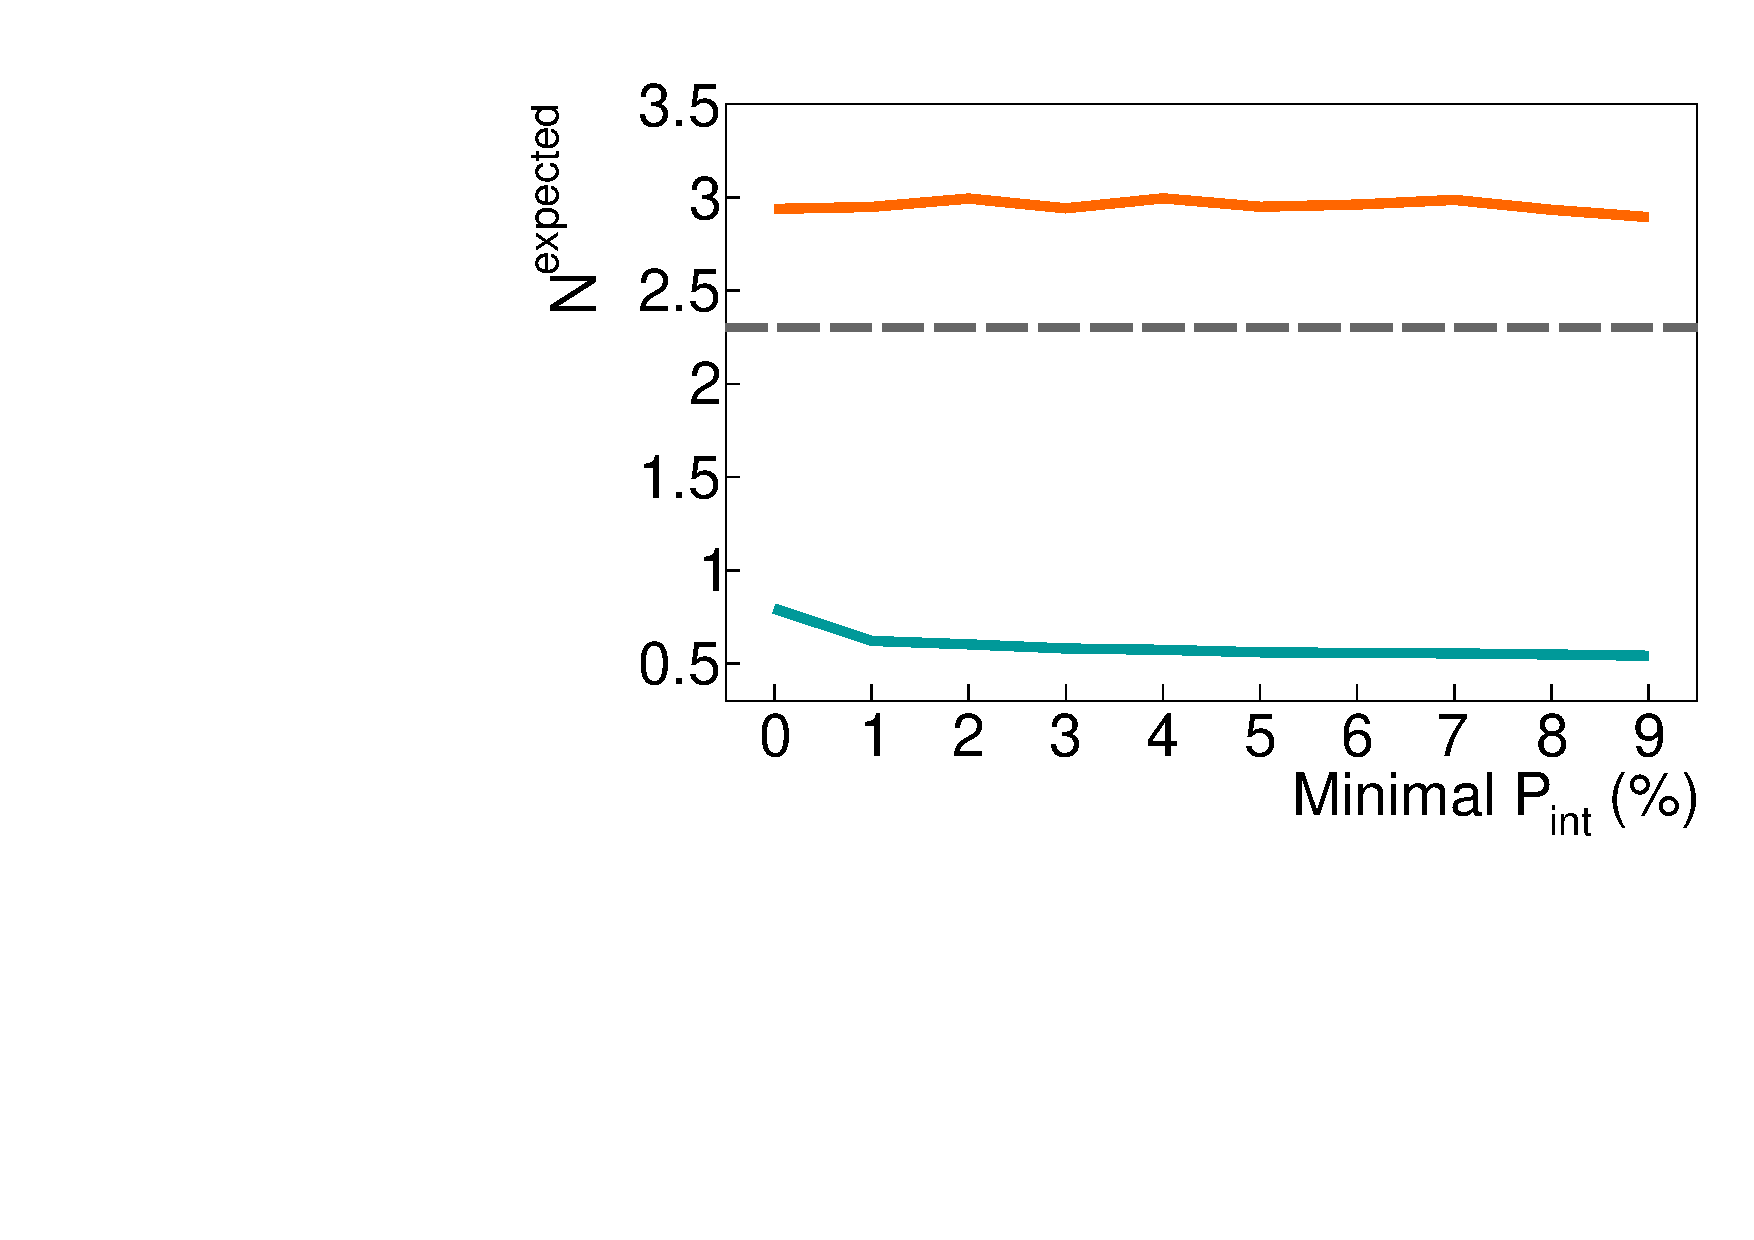
\includegraphics[width=0.82\textwidth]{Sensitivity/fig_sensitivity/82Se_cont_cut_nexcl_B.pdf}
  \captionsetup{justification=centering}
  \caption{Total expected number of background in ROI.
    \label{subfig:cont_Pint_Nexp}}
\end{subfigure}
\hfill
\begin{subfigure}[t]{0.49\textwidth}
  \centering
  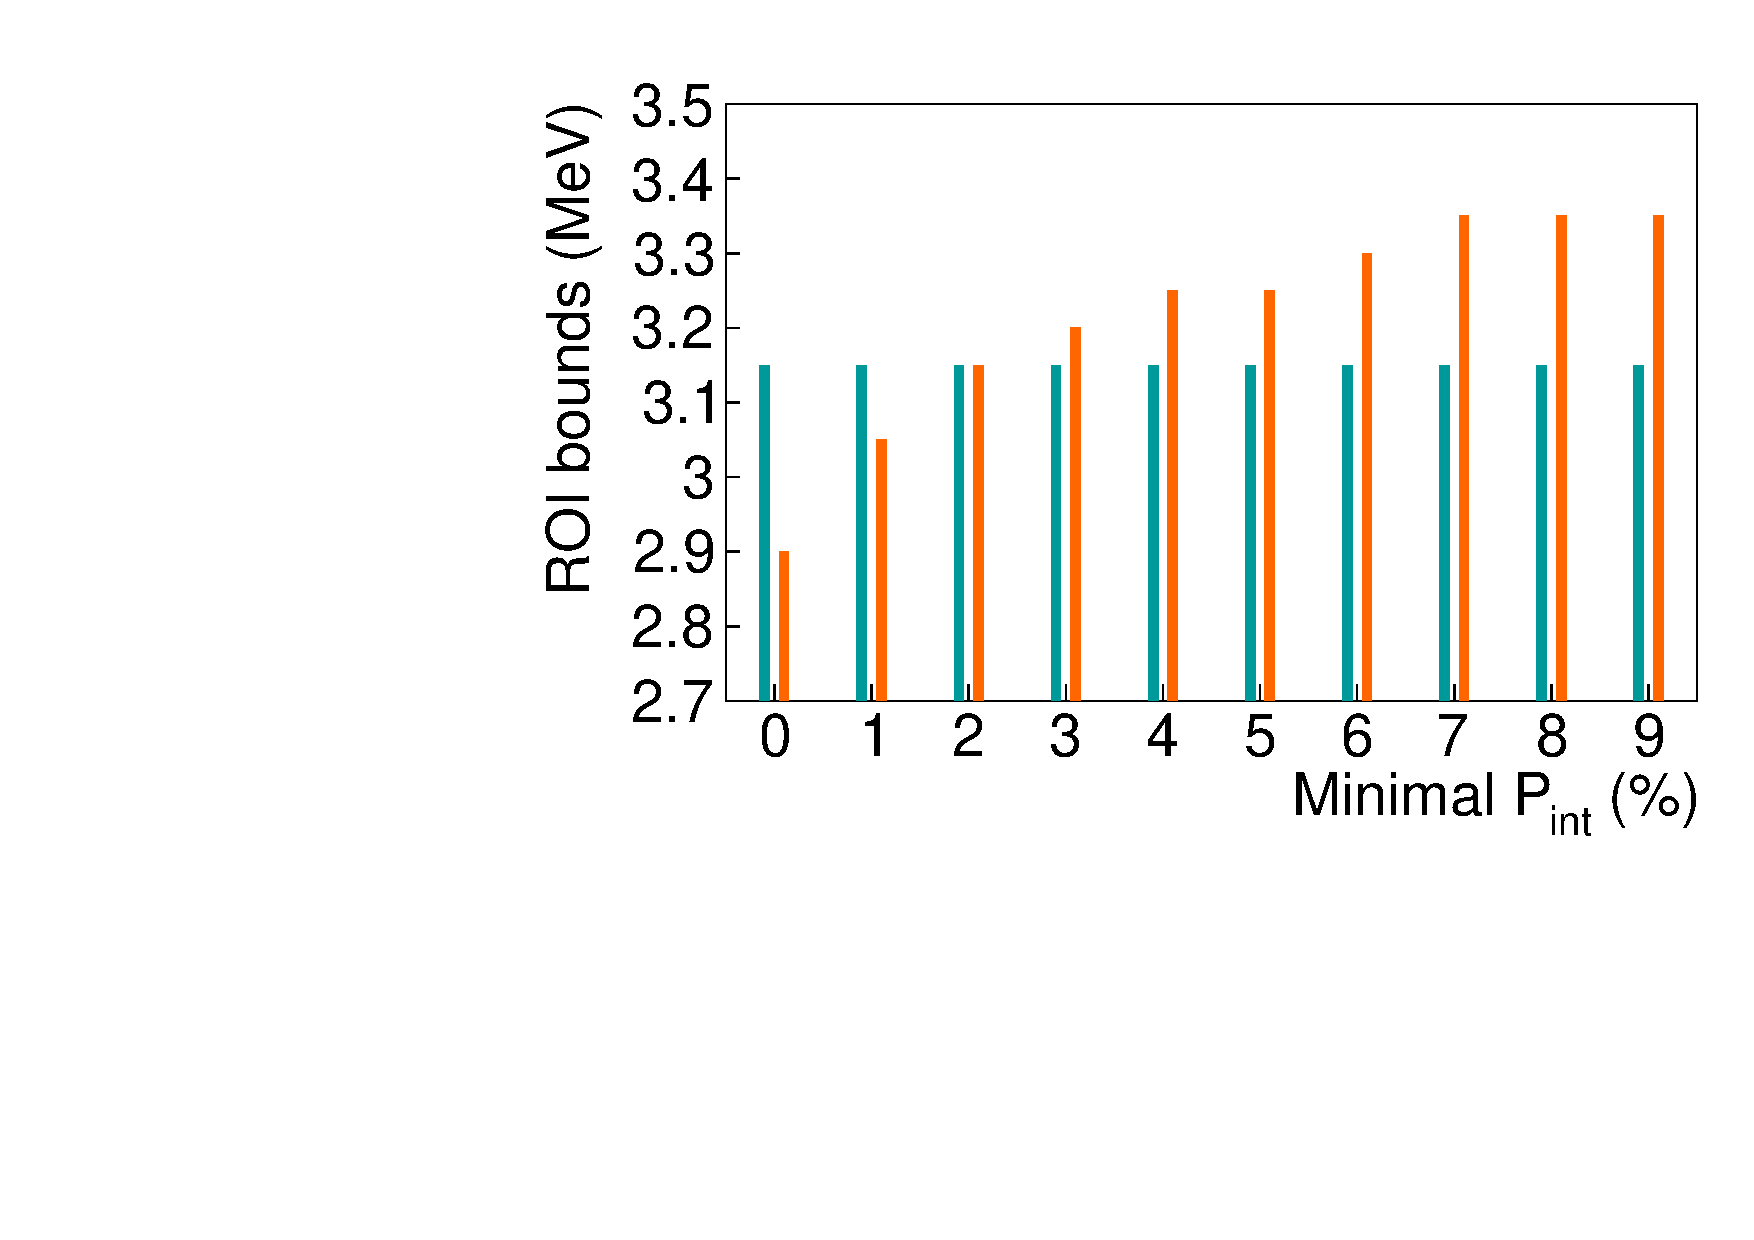
\includegraphics[width=0.82\textwidth]{Sensitivity/fig_sensitivity/ROI_cut_Pint_B.pdf}
  \captionsetup{justification=centering}
  \caption{ROI optimisation.
    \label{subfig:cont_Pint_ROI}}
\end{subfigure}
\vskip\baselineskip
\begin{subfigure}[t]{0.49\textwidth}
  \centering
  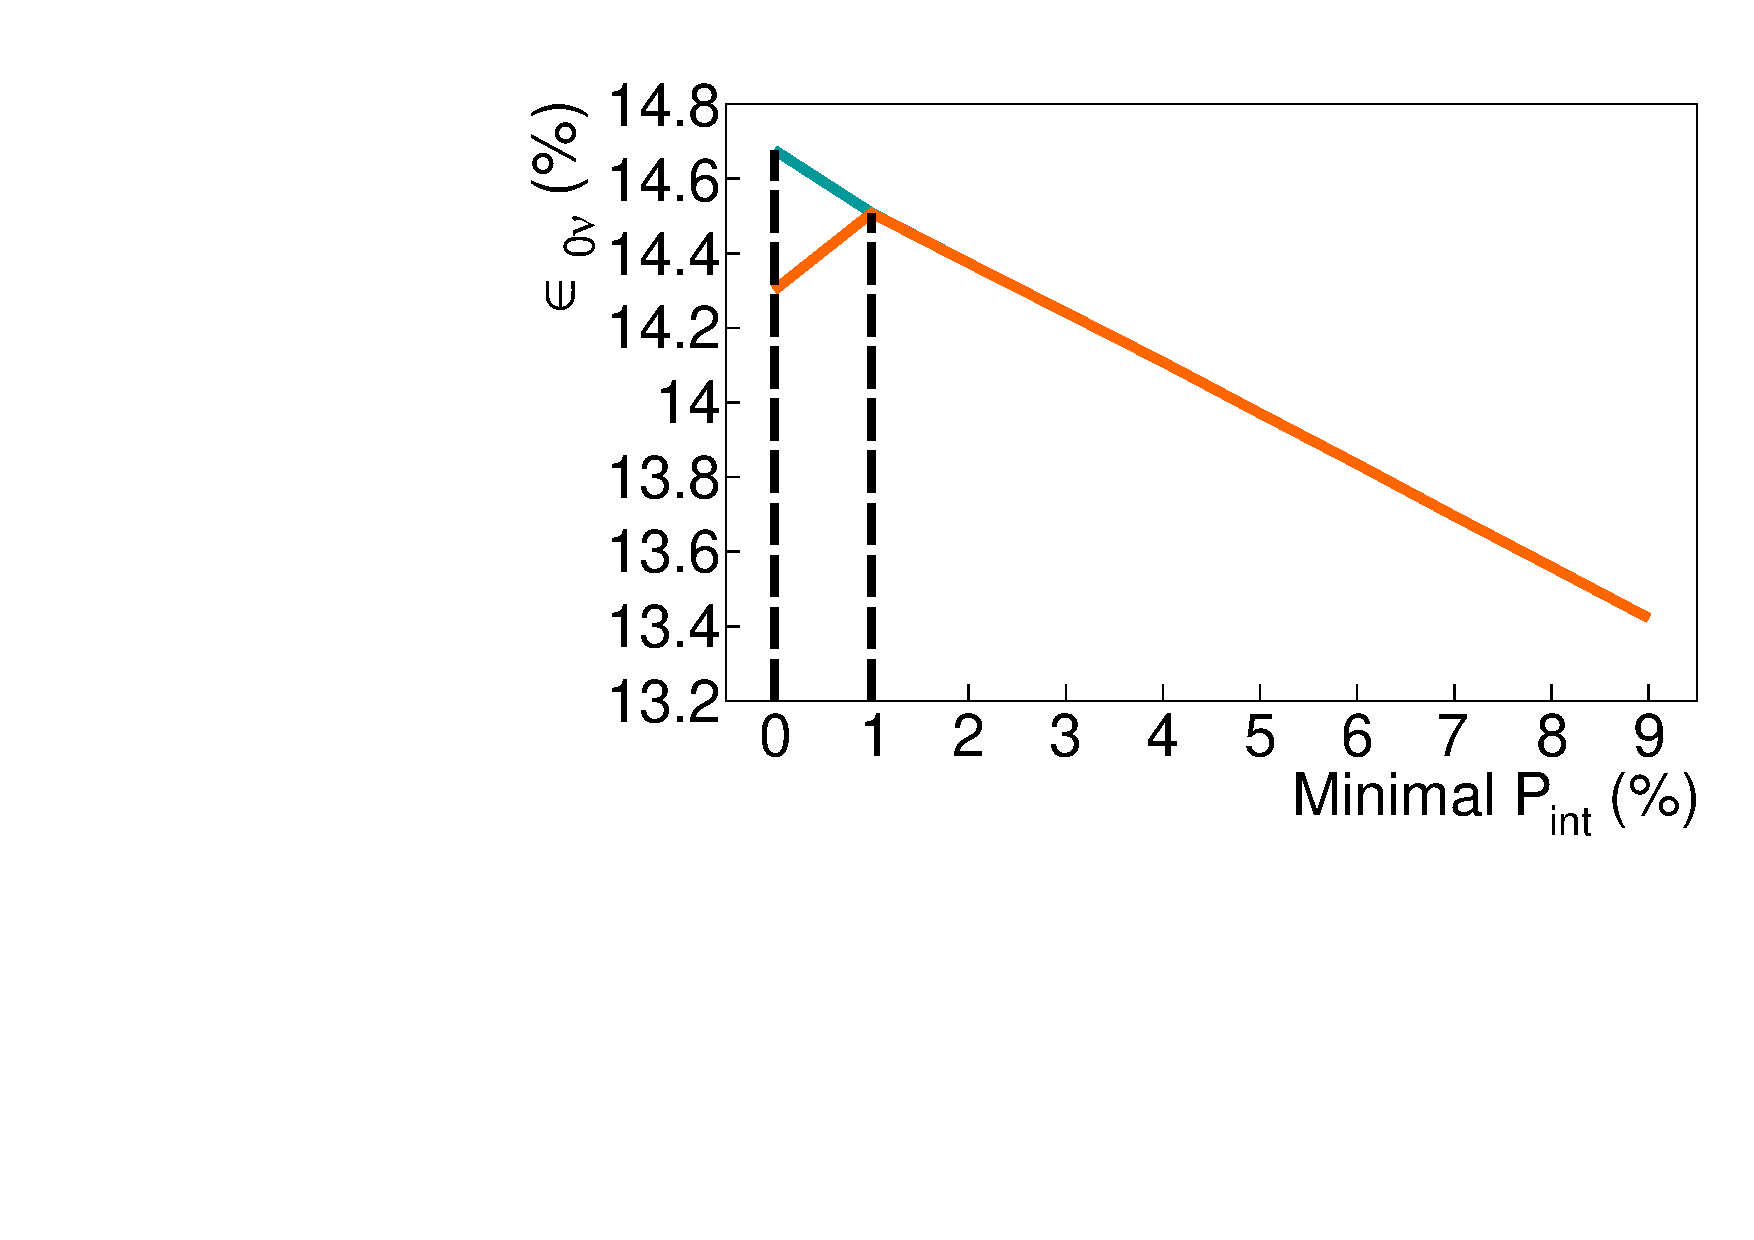
\includegraphics[width=0.82\textwidth]{Sensitivity/fig_sensitivity/cont_cut_eff_B.pdf}
  \captionsetup{justification=centering}
  \caption{$\zeronu$ selection efficiency in ROI.
    \label{subfig:cont_Pint_eff}}
\end{subfigure}
\hfill
\begin{subfigure}[t]{0.49\textwidth}
  \centering
  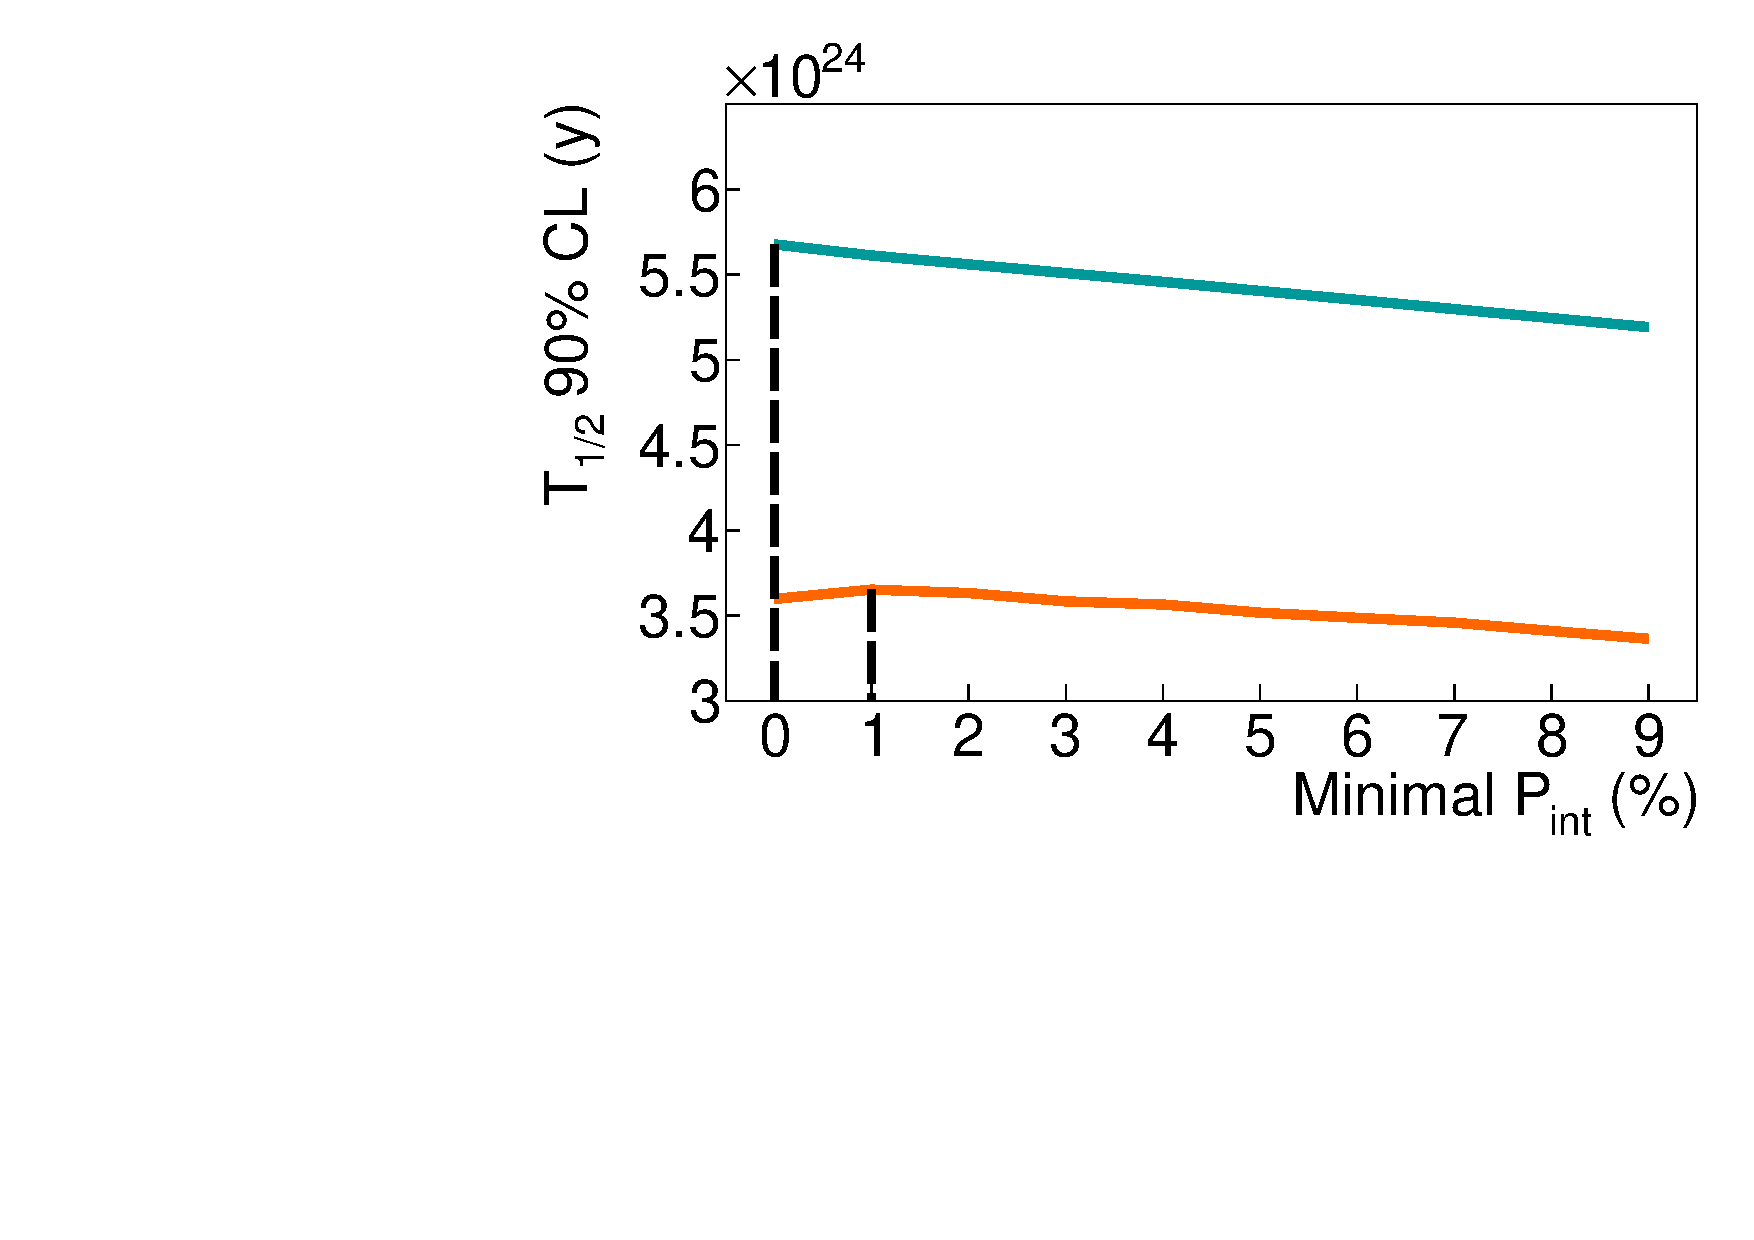
\includegraphics[width=0.82\textwidth]{Sensitivity/fig_sensitivity/cont_cut_T12_B.pdf}
  \captionsetup{justification=centering}
  \caption{Limit on $\Tbeta$.
    \label{subfig:cont_Pint_T12}}
\end{subfigure}
\vskip\baselineskip
\begin{subfigure}[t]{0.49\textwidth}
  \centering
  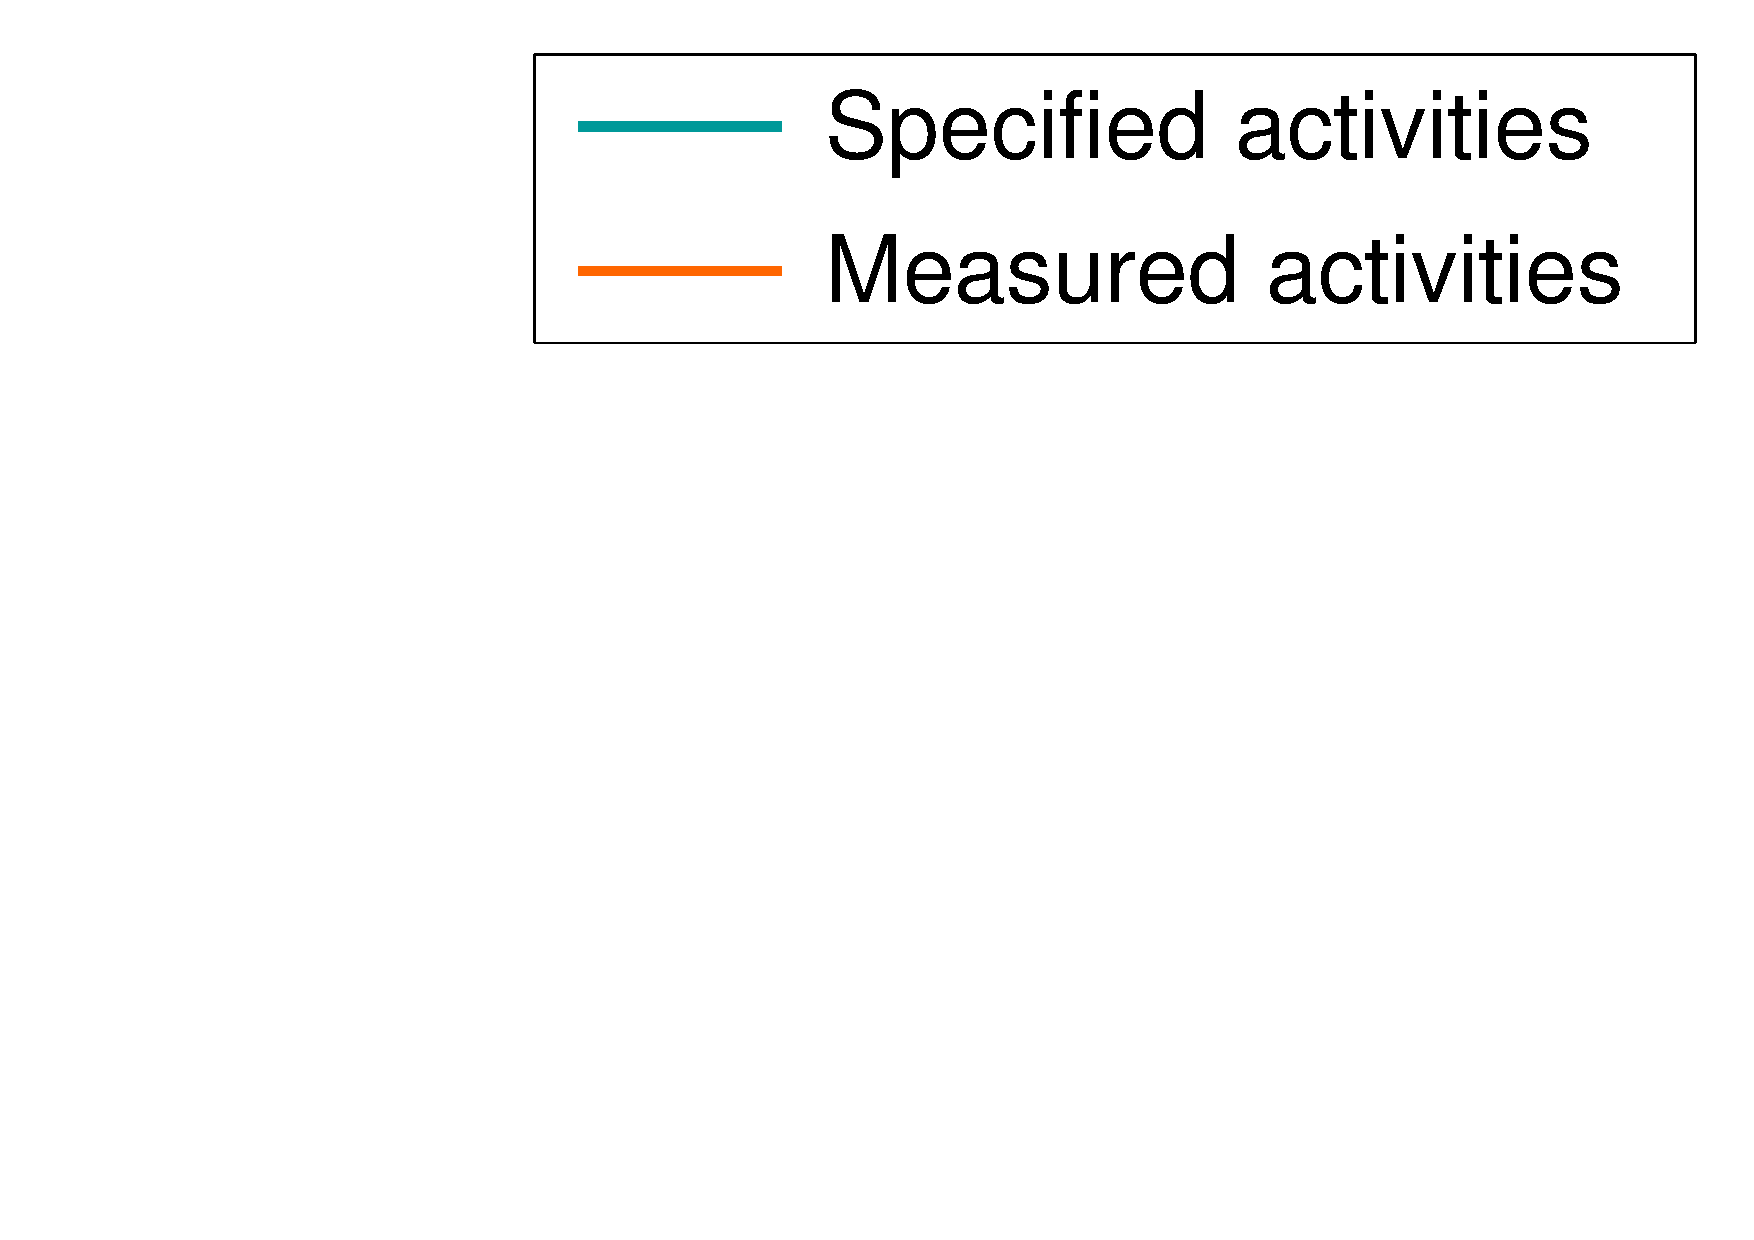
\includegraphics[width=0.5\textwidth]{Sensitivity/fig_sensitivity/legend_cut_Pint.pdf}
  \end{subfigure}
\caption{Total number of expected background in ROI (a),
  evolution of the regions of interest (b),
  $\zeronu$ selection efficiency in ROI (c),
  and limit set on $\Tbeta$ at $90\%$ CL (d),
  as a function of the cut-off applied on internal probability, \Pint.
  The ROI is optimised for each \Pint\ value.
  Results are displayed for two contamination levels: the specified (blue) and the measured (orange) activities (taking into account the upper limit provided for \Bi).
  An exposure of $17.5$~kg.y is considered.
  Two vertical dashed lines in (c) and (d) display the best \Pint\ selections to be applied in order to improve the $\Tbeta$ sensitivity of the experiment.
  \label{fig:cont_Pint}}
\end{figure}
We consider two levels of contamination, the specified and measured contamination levels (taking the upper limit for \Bi).
We first detail these figures for the case of the specified activities and then explain what we observe for the measured activities.

\paragraph{Specified activities}
The total expected number of background in the ROI (Fig.~\ref{subfig:cont_Pint_Nexp}) is very low compared to one, smaller than $0.8$ for \Pint$>0$\%, and constantly decreases when the minimal cut on \Pint\ increases.
Therefore, the number of excluded signal events, $N_{0\nu}^{\text{excl.}}$, is set to its minimal value of $2.303$, regardless of the \Pint\ level.
As a consequence, the ROI bounds are stable (Fig.~\ref{subfig:cont_Pint_ROI}).
As the ROI do not influence the selection efficiencies, $\epsilon_{0\nu}$ is only impacted by the \Pint\ level applied, and decreases with it (Fig.~\ref{subfig:cont_Pint_eff}).
All these observation allow to understand the evolution of $\Tbeta$ (Fig.~\ref{subfig:cont_Pint_T12}), decreasing with the \Pint\ level applied on simulations.
The sensitivities displayed for a $0\%$ cut-off on P$_{\text{int}}$ of course correspond to the results given in Fig.~\ref{fig:real_target_act}.

\paragraph{Measured activities}

The total number of expected background event is, naturally, higher than for the specifications, and above all is greater than the $2.303$ limit.
Nevertheless, this level is too low for the \Pint\ cut-off to have an impact, and the number of expected background remains constant.
When the minimal acceptable \Pint\ is changed from $0$ to $1$~\%, the ROI upper bound increases from $2.9$ to $3.05$~MeV.
Usually, the variation of this bound does not have such a great impact on the event selection.
Nevertheless, in the measured activities case, for a \Pint~$>~0~\%$ level, the ROI is optimised at the narrow [$2.7$;$2.9$]~MeV interval, where the upper bound is located in an energy region still populated by signal (see Fig.~\ref{fig:real_target_act}).
Therefore, even small variations in this ROI has a great impact on the $\zeronu$ selection efficiency, explaining this local increase.
We then observe a slight increase of $\zeronu$ selection efficiency for the level \Pint$>1\%$.
For \Pint\ selections greater than $1~\%$, we come back in cases where the upper bound of the ROI no longer has an impact on $\epsilon_{0\nu}$.
At this level, only variations of the total number of background events, showed in Fig.~\ref{subfig:cont_Pint_Nexp} have an impact.
As the limit set on $\Tbeta$ depends directly on $\epsilon_{0\nu}$, the variations presented in Fig.~\ref{subfig:cont_Pint_eff} fully explain the results displayed in Fig.~\ref{subfig:cont_Pint_T12}, presenting the evolution of $\Tbeta$ with the internal probability selection level.

The optimisation work we have just presented is of interest in the case of measured activities, where the cut-off on \Pint\ is set at $1$\%.
We will see in the following sections that this optimisation is also be useful, especially when studying the influence of the magnetic field.
However, this rejection criterion has only a limited impact on the improvement of $\Tbeta$ sensitivity for the specified activities, because of the very low contamination levels considered.
Indeed, paradoxically, the selection on internal probability worth it only if there is enough background events to be rejected, as we can start observing for the measured activities case.
Nevertheless, in that case, we recommend to keep at least a loose cut-off at \Pint$>4~\%$.
Indeed, this only slightly degrades the sensitivity (around $4$\%) while insuring the rejection of potential harmful external backgrounds for a more general study.



\subsubsection{Vertices distance}

NEMO-$3$ analyses also used the distance between the reconstructed vertices on the source foils as a background rejection criterion.
As we have shown that the additional \Pint\ cut-off is poorly adapted for the low activities of SuperNEMO sources, it is interesting to know if we can improve the results by using this second selection.
Thanks to the trajectory fitting algorithm, we have access to the ($Y,Z$) coordinates of the latter, and by extension, to the distance between them.
In the previous studies, the choice was made to look at the effect of this selection, separately on the $Y$ (perpendicular to the wires) and $Z$ (parallel to the wires) directions.
We choose to follow the same approach, and we give the results for a cut along the $Z$ axis, but the conclusions would remain valid for the $Y$ direction.
Fig.~\ref{fig:vertex_dist} shows the distributions of the absolute value of the distance between foil vertices for each process studied.
\begin{figure}[h!]
  \centering
  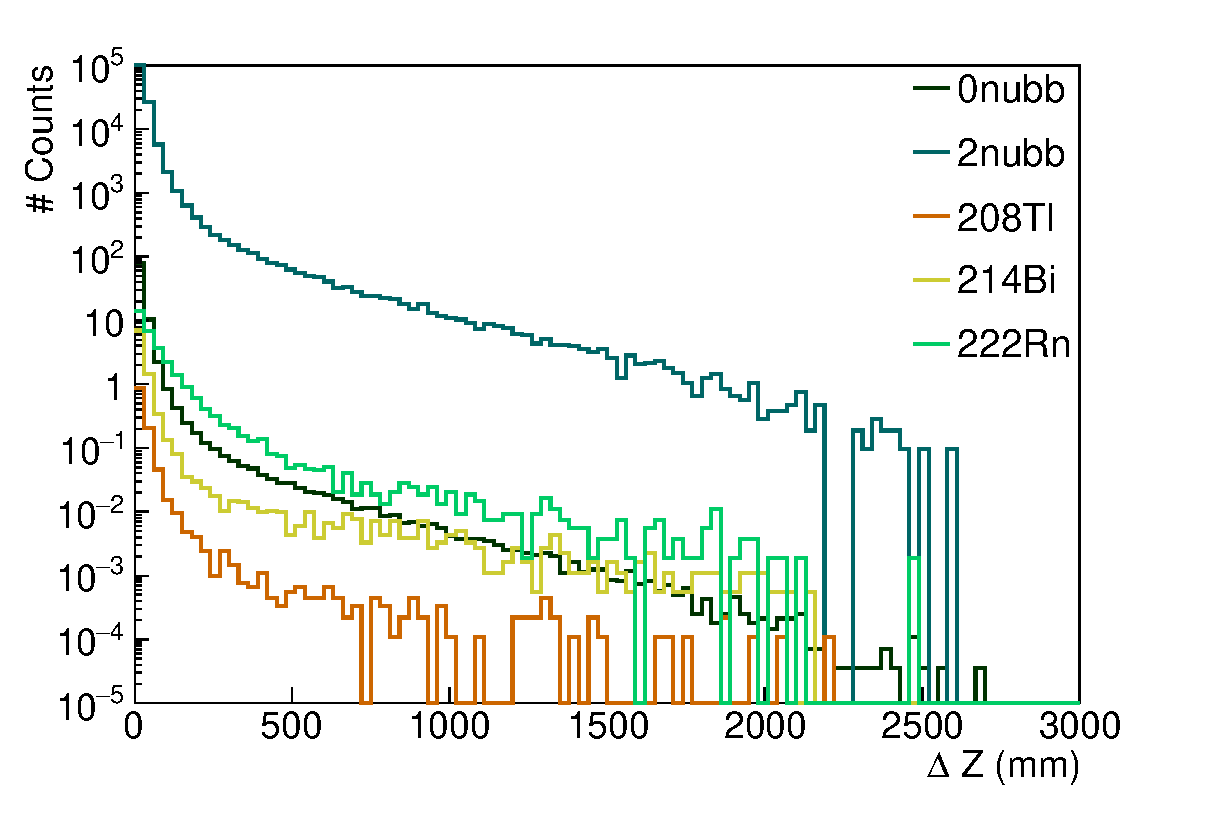
\includegraphics[width=0.8\textwidth]{Sensitivity/fig_sensitivity/Vertex_distance.eps}
  \caption{Distance along the $Z$ direction between the vertices of the $2$ reconstructed electrons, for each process considered.
    The $\twonu$ spectrum is normalised to $\Ttwonu~=~9.39\times~10^{19}$~y, and \Tl, \Bi\ and \Rn\ backgrounds are normalised to the nominal activities.
    The amplitude of the $\zeronu$ is arbitrarily set at the $90$\% limit obtained with NEMO-$3$.
    No energy cut is applied.
    \label{fig:vertex_dist}}
\end{figure}
We would use this information in order to maximise the double $\beta$ decays to be selected, while rejecting natural isotope disintegrations.

In the same way as the previous paragraph, Fig.~\ref{fig:cont_vertex} displays all informations leading to the maximisation of $\Tbeta$, allowing to study the impact of the vertices distance cut-off on the final sensitivity.
\begin{figure}[!h]
\centering
\begin{subfigure}[t]{0.49\textwidth}
  \centering
  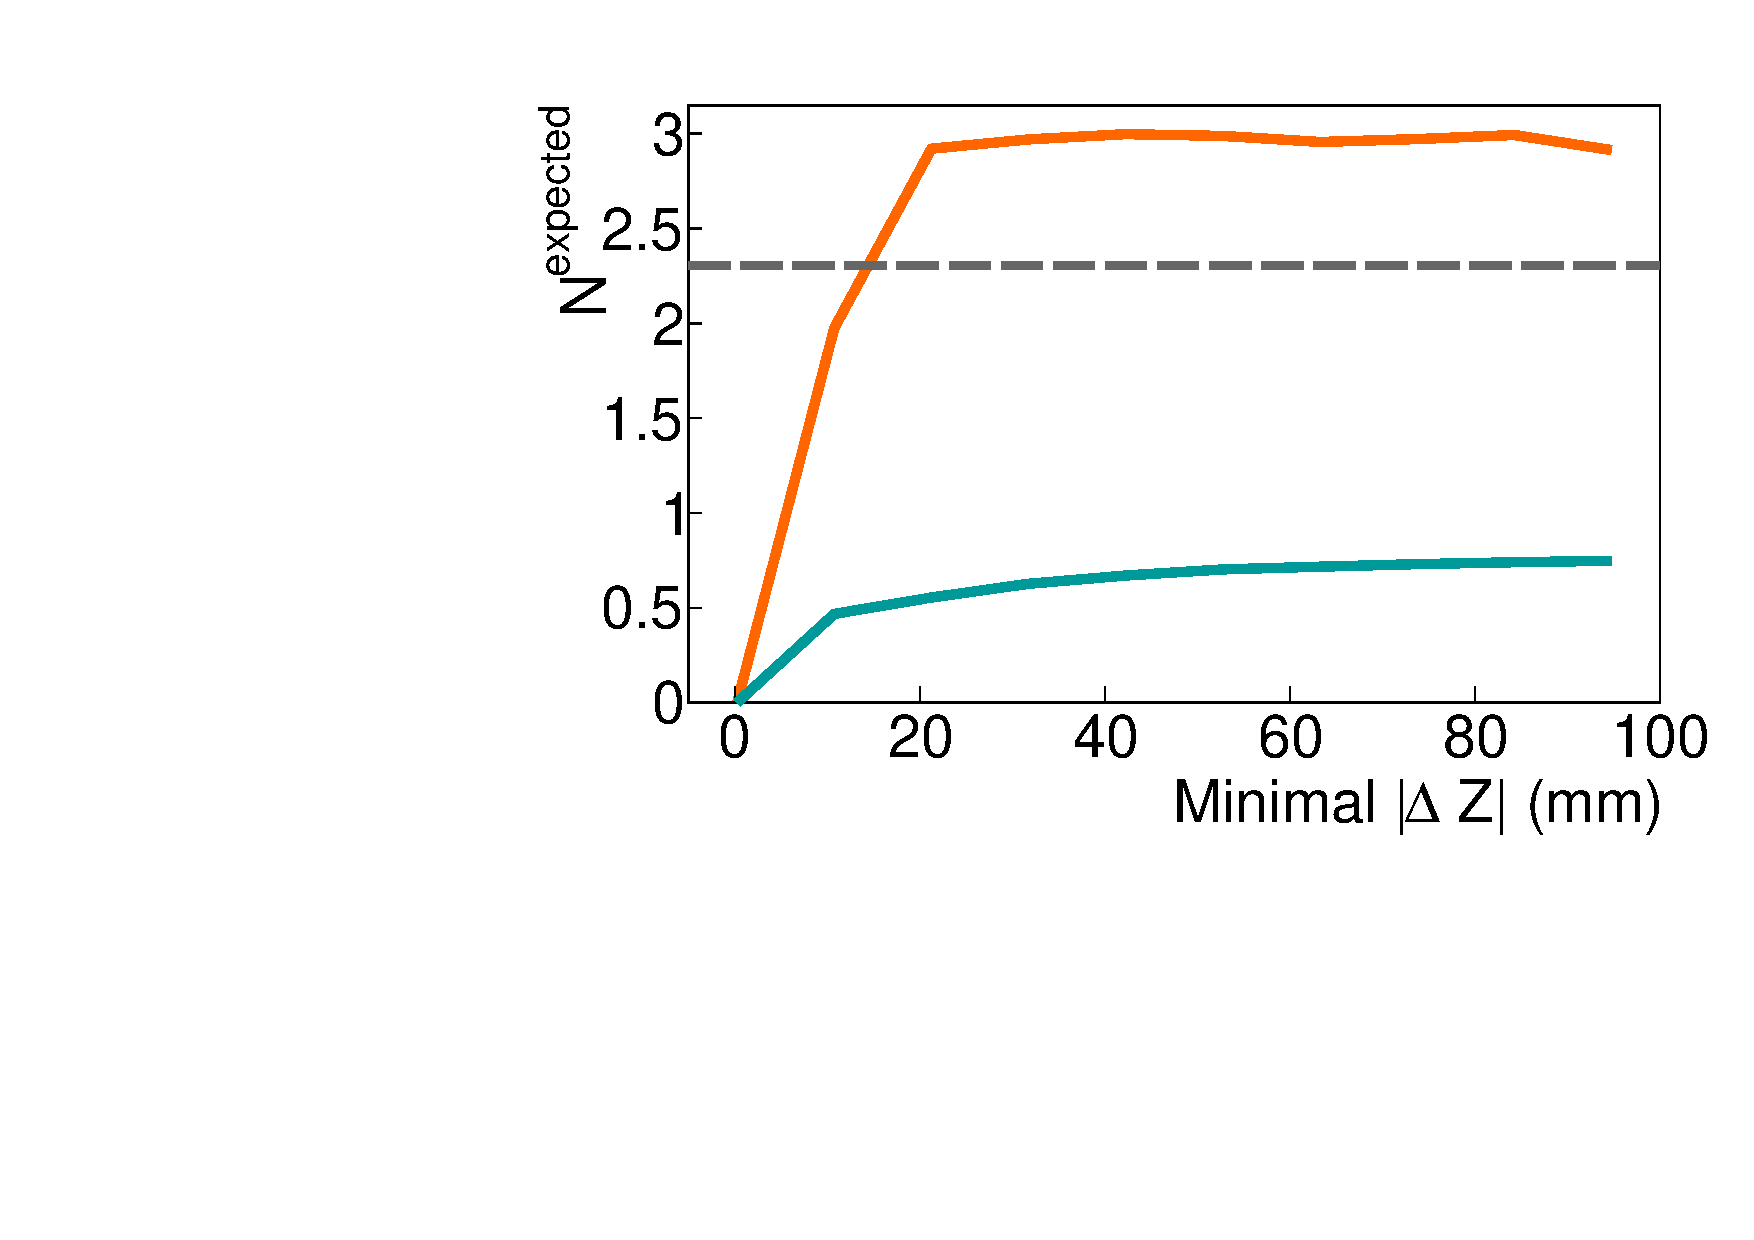
\includegraphics[width=0.82\textwidth]{Sensitivity/fig_sensitivity/82Se_cont_cut_vertex_nexcl_B.pdf}
  \captionsetup{justification=centering}
  \caption{Total expected number of background.
    \label{subfig:cont_vertex_Nexp}}
\end{subfigure}
\hfill
\begin{subfigure}[t]{0.49\textwidth}
  \centering
  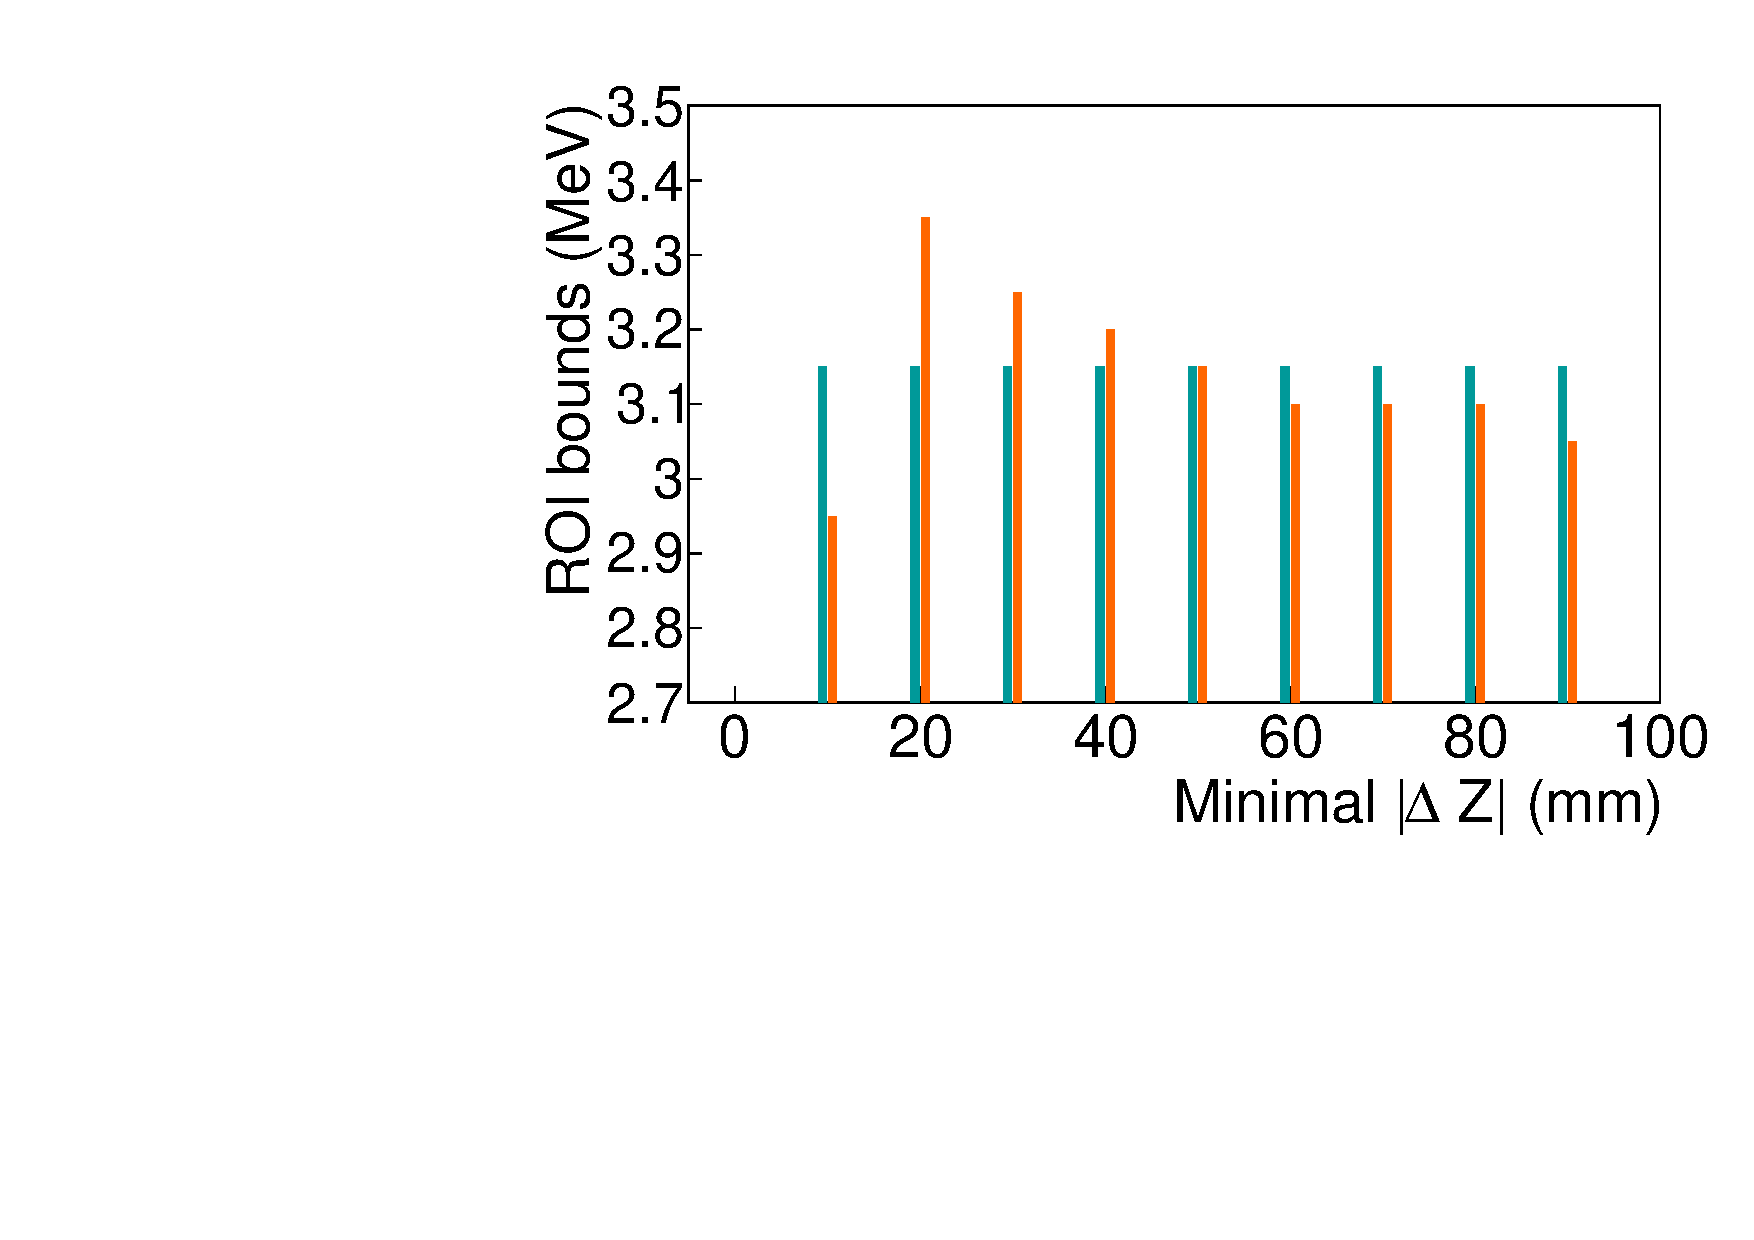
\includegraphics[width=0.82\textwidth]{Sensitivity/fig_sensitivity/82Se_ROI_cut_vertex_B.pdf}
  \captionsetup{justification=centering}
  \caption{ROI optimisation.
    \label{subfig:cont_vertex_ROI}}
\end{subfigure}
\vskip\baselineskip
\begin{subfigure}[t]{0.49\textwidth}
  \centering
  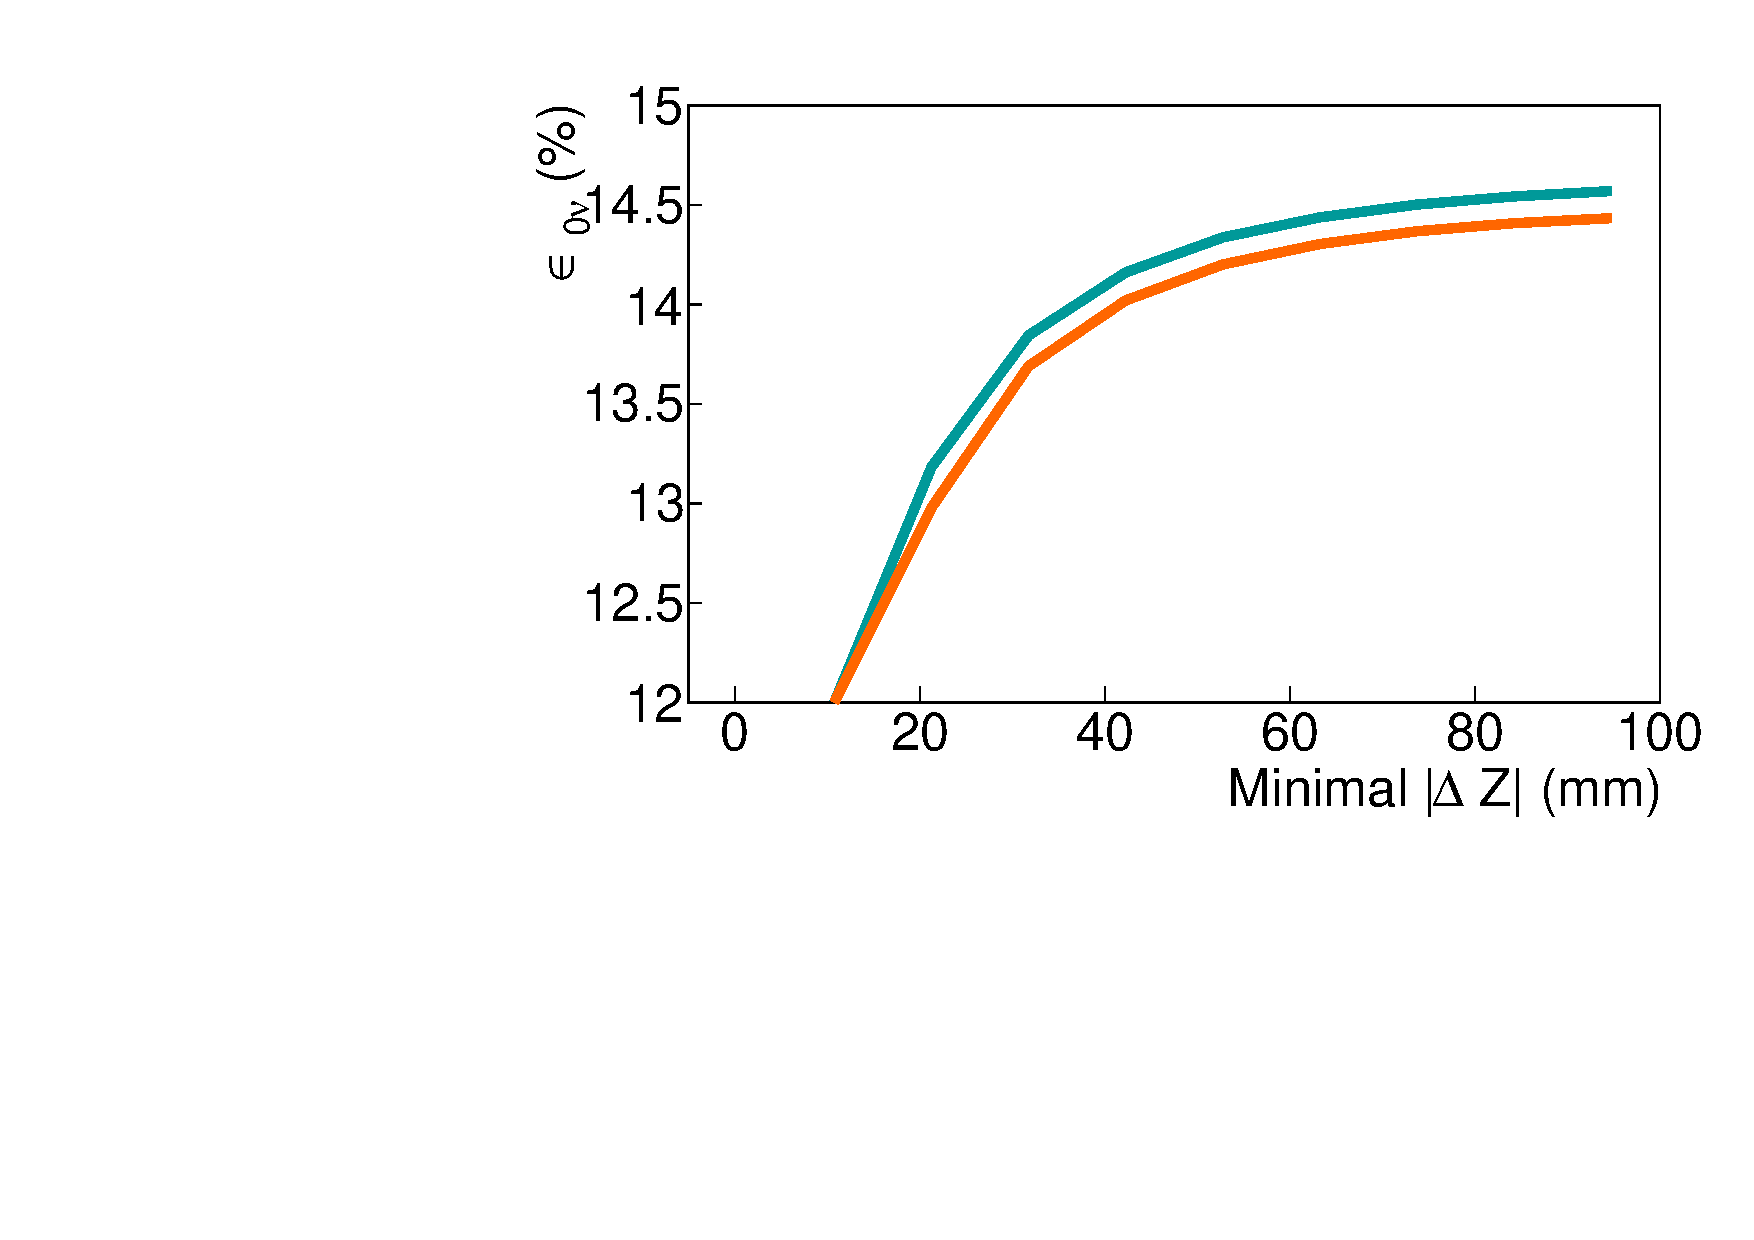
\includegraphics[width=0.82\textwidth]{Sensitivity/fig_sensitivity/82Se_cont_cut_vertex_eff_B.pdf}
  \captionsetup{justification=centering}
  \caption{$\zeronu$ selection efficiency.
    \label{subfig:cont_vertex_eff}}
\end{subfigure}
\hfill
\begin{subfigure}[t]{0.49\textwidth}
  \centering
  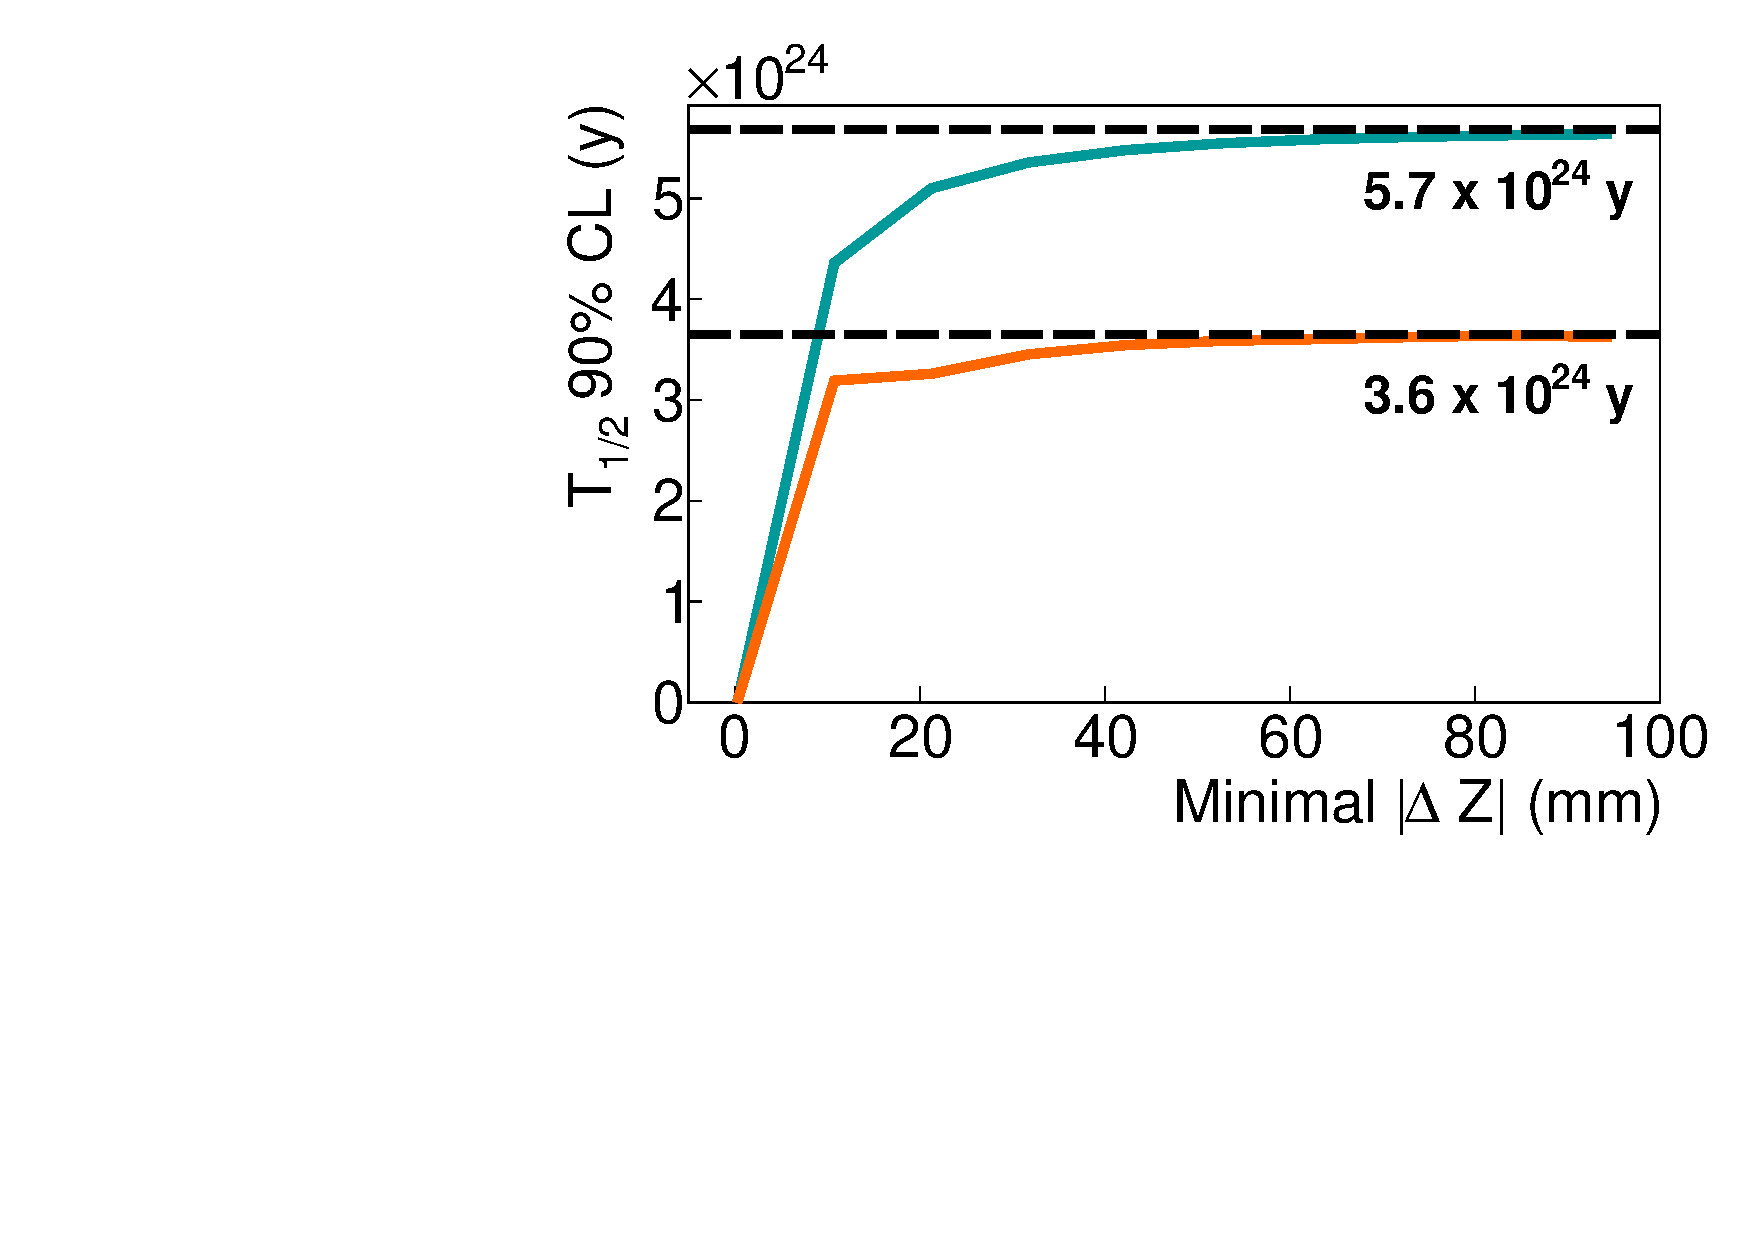
\includegraphics[width=0.82\textwidth]{Sensitivity/fig_sensitivity/82Se_cont_cut_vertex_T12_B.pdf}
  \captionsetup{justification=centering}
  \caption{Limit on $\Tbeta$.
    \label{subfig:cont_vertex_T12}}
\end{subfigure}
\vskip\baselineskip
\begin{subfigure}[t]{0.49\textwidth}
  \centering
  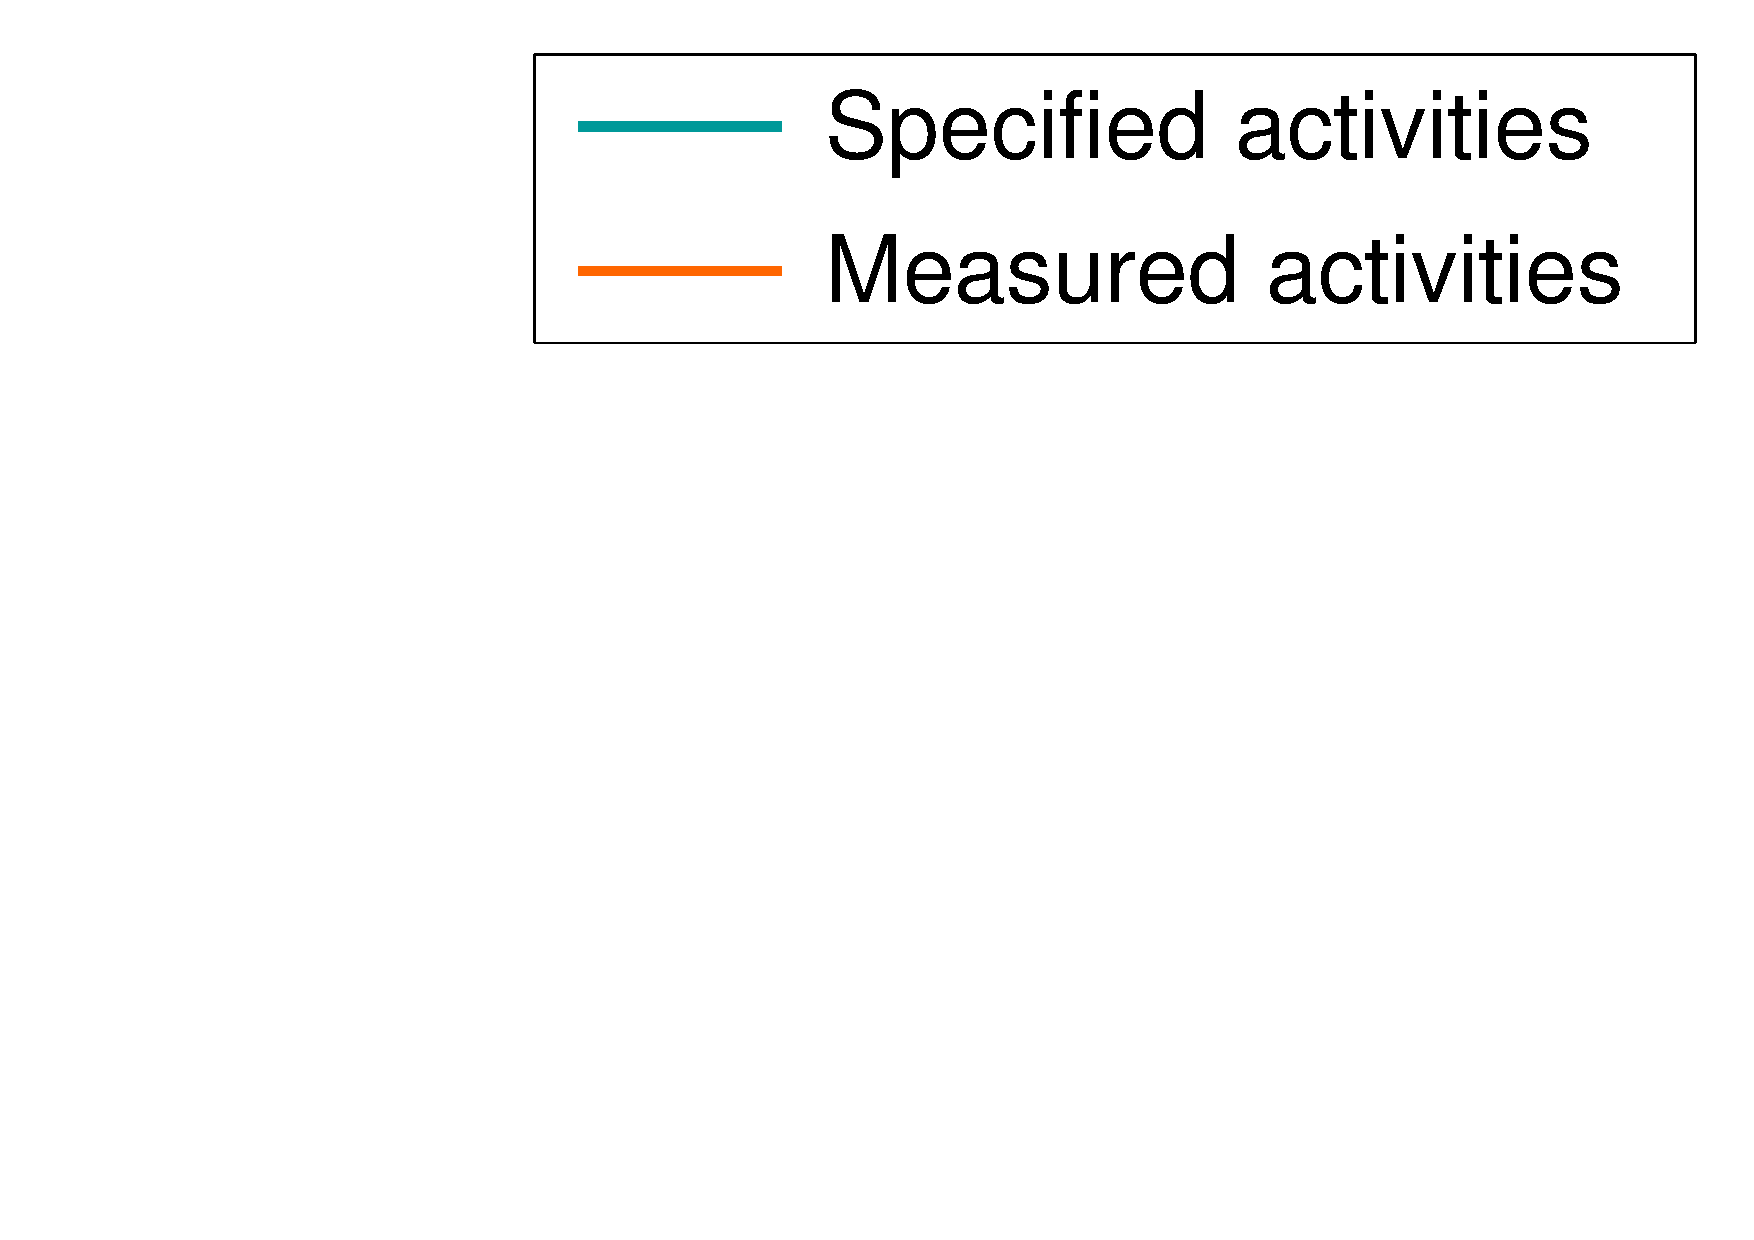
\includegraphics[width=0.5\textwidth]{Sensitivity/fig_sensitivity/legend_cut_Pint.pdf}
  \end{subfigure}
\caption{Total number of expected background in ROI (a),
  evolution of the regions of interest (b),
  $\zeronu$ selection efficiency in ROI (c),
  and limit set on $\Tbeta$ at $90\%$ CL (d),
  as a function of the cut-off applied on distance between vertices, $|~\Delta Z~|$.
  The ROI is optimised for each $|~\Delta Z~|$ cut.
  Results are displayed for two contamination levels: the specified (blue) and the measured (orange) activities (taking into account the upper limit provided for \Bi).
  An exposure of $17.5$~kg.y is considered.
  \label{fig:cont_vertex}}
\end{figure}
Overall, these figures show us that too strict cut-off on the distance between vertices would lead to a decrease in sensitivity.
Because of the variations of the $\zeronu$ selection efficiency and the total number of background events, the $\Tbeta$ distributions reaches a plateau, corresponding to the sensitivities achieved with the first-order cuts and optimised \Pint.
In practice, as it is done for \Pint, a selection on vertex distance will always be applied, even if it is very loose, as such a cut-off could be useful for rejecting unexpected background (coincidence between independent events, for instance).
We recommend to apply a loose cut-off level at $|~\Delta Z~|~<~80$~mm, which does not degrade significantly the sensitivity.
The same conclusions apply to the $|~\Delta Y~|$ cut-off.


\paragraph{}The idea of having implemented these two selections (on the internal probability and on the distance between vertices) comes from a previous NEMO-$3$ analysis on the background rejection.
For the SuperNEMO demonstrator case, the levels of contaminations we are dealing with is remarkably low for most of the topological cut-offs to be worth applying.
However, in practice, applying loose topological selections on the data remains necessary, especially to reject external background events.
The minimal cut-off level to be applied is \Pint~$>~4~\%$ and $|~\Delta~Z~|~<~80$~mm (similarly for $|~\Delta~Y~|$), and can be optimised by taking into account the sources activity.

For future studies, it is useful to give the efficiencies of these loose selections, for the signal and for each background considered (Tab.~\ref{tab:Pint_eff}), as well as the expected number of background in the ROI (Tab.~\ref{tab:Nexp_topo_contamination}).
\begin{table}[h]
  \begin{subtable}[h]{1.\textwidth}
    \centering
    \begin{tabular}{|c|c|c|c|}
      \hline
      Cut-off & First-order cuts (\%) & Internal probability (\%) & Vertex distance (\%) \\
      && \Pint$~>~4\%$ & $|~\Delta~Z~|~<~80$~mm \\
      \hline\hline
      $\zeronu$  & $26.9$ & $25.3$ & $24.7$ \\
      $\twonu$  & $9.15$ & $8.56$ & $8.21$ \\
      \Tl  & $0.106$ & $0.0889$ & $0.0846$ \\
      \Bi  & $0.168$ & $0.151$ & $0.144$ \\
      \Rn  & $0.0177$ & $7.91\times~10^{-3}$ & $5.34\times~10^{-3}$ \\
      \hline
    \end{tabular}
    \captionsetup{justification=justified}
    \caption{Selection efficiencies for the three levels of selection (first-order, \Pint\ and vertex distance), in the full energy range.
      \label{tab:Pint_eff}}
  \end{subtable}
  \vskip\baselineskip
  \begin{subtable}[h]{1.\textwidth}
    \begin{tabular}{|c|c|c|c|c|}
      \hline
      Activity & \multicolumn{2}{c|}{Specified} & \multicolumn{2}{c|}{Measured (w/ \Bi)} \\
      \hline
      Cut-off & \Pint~$>~4~$\% & $|~\Delta~Z~|~<~80$~mm & \Pint~$>~4~$\% & $|~\Delta~Z~|~<~80$~mm  \\
      ROI (MeV) & [$2.7$;$3.15$] & [$2.7$;$3.15$] & [$2.7$;$3.25$] & [$2.7$;$3.3$] \\
      \hline\hline
      $\epsilon_{0\nu}$ & $14.1$\% & $13.9$\% & $14.1$\% & $13.9$\% \\
      \hdashline
      $\twonu$  & $0.392$ & $0.383$ & $0.392$ & $0.383$ \\
      \Tl  & $0.0338$ & $0.0323$ & $1.08$ & $1.09$ \\
      \Bi  & $0.0491$ & $0.0491$ & $1.42$ & $1.42$ \\
      \Rn  & $0.115$ & $0.0782$ & $0.115$ & $0.0782$ \\
      Total & $0.590$ & $0.543$ & $3.01$ & $2.97$ \\
      \hline
    \end{tabular}
    \captionsetup{justification=justified}
    \caption{Selection efficiency of $\zeronu$ events and expected number of backgrounds events in the optimised ROI, for the exposure of the SuperNEMO demonstrator (17.5 kg.y), for successive application of topological selections.
      Specified and measured activities (taking into account the upper limit for \Bi\ contamination) are considered.
      \label{tab:Nexp_topo_contamination}}
  \end{subtable}
  \caption{The selection efficiencies and expected number of background events for the topological selections.}
\end{table}
As detailed, regions of interest are optimised for each selection.
The selection efficiencies show topological cuts have a huge impact on Radon selection, as they are especially designed to reject non-internal events.
The \Pint\ cut-off is also efficient in rejecting Thallium internal events, because of the existence of a metastable exited state, described earlier.
A special technique to reject efficiently \Tl\ background is also addressed in Chapter~\ref{ch:timediff}.

After the topological cut-off optimisation, the SuperNEMO demonstrator would reach a sensitivity of $\Tbeta~>~5.4\times~10^{24}$~y if specified activities are reached, corresponding to the effective neutrino mass range $\langle\mbb\rangle~<~[0.25-0.48]$~eV.
For the measured activities, supposing \Bi\ activity reaches the measured upper limit, $\Tbeta~>~3.6\times~10^{24}$~y and $\langle\mbb\rangle~<~[0.31-0.59]$~eV.

In the following we review the influence of the $25$~Gauss magnetic field inside the detector on the sensitivity reachable by the SuperNEMO demonstrator.

\section{Impact of the magnetic field on the sensitivity}
\label{subsec:field}

The SuperNEMO demonstrator was originally designed with a copper coil, similarly to NEMO-$3$, delivering a magnetic field inside the tracker volume.
This $25$~Gauss magnetic field is high enough to bend the trajectory of the few~MeV electrons and positrons of interest for SuperNEMO, without too strongly preventing them from reaching the calorimeter.
In practice, this magnetic field is mainly used to identify and reject the electron-positron pairs created by high energy $\gamma$’s, themselves emitted after a neutron capture.
However, as explained in sub-section~\ref{subsec:ext_bkg}, we choose to not consider the contribution of this external background for this study's background model.
We therefore focus on evaluating the influence of the presence of the magnetic field on the rejection of natural isotopes contaminating the source foils and wire chamber.
%% It is also very useful to better identify the crossing electron events, mostly coming from a 212 Bi contamination on the surface of the calorimeter, as explained in Section 3.2.4.
%% For instance, as shown in Figure 4.1, NEMO-3 observed three events in the [2.8;3.2]MeV region of interest in the one electron one positron channel and two events, induced by high energy $\gamma$’s from neutron capture, with energies higher than 4~MeV.


%% As described in Sec.~\ref{sec:magnetic_field}, the presence of a magnetic field of $25$ G could influence the optical modules performances.
%% In the simulated detector, such effects are not yet implemented, therefore can't be observed in the framework of this analysis.
%% However, possible degradation of the event reconstruction efficiency.



\subsection{Simulations of the magnetic field}

In order to study the influence of the magnetic field on the demonstrator sensitivity to the $\zeronu$ decay, the simulations and reconstructions of signal and backgrounds have been performed in two different conditions.
\begin{itemize}
\item Simulations with a uniform $25$ Gauss magnetic field (following recommendations \cite{CalvezThesis}).
  Results about the final sensitivity achieved in this condition have already been presented earlier in this chapter.
  The possible variations of the field intensity, mainly due to the calorimeter magnetic shields, are not taken into account for these simulations.
  This will be discussed in sub-section~\ref{subsec:mapped_field}.
\item Simulations where the magnetic field is turned off.
%\item simulations with a $25$ Gauss \emph{mapped} magnetic field, taking into account more realistic variations of the magnetic field inside the detector~\cite{docdb:map_magnetic_field2015}.
\end{itemize}
Each magnetic field condition has the same number of simulated events, as summed up in Tab.~\ref{tab:sensitivity_simulations}.

Depending on the case under consideration, the charged particles do not have the same trajectory curvature.
In the first uniform on-field case, they are bended.
The track fit algorithm then performs two distinct trajectory fittings: one with a helix and one with a line.
The most accurate fit is chosen and provides information on the charge of the detected particle.
In the second off-field case, the fitting algorithm is modified to match line trajectories.
%Finally, the best tracking option (line or helix) for the third mapped on-field case is discussed in the next section.

\subsection{Impact of the magnetic field on signal and background selections}
\label{subsec:impact_field}
%%%

Among first-order event selection criteria considered in Sec.~\ref{sec:sensitivity_ev_selection}, the one on the trajectory curvature is of primary importance with regard to the influence of the magnetic field on the final sensitivity.
Indeed, when the magnetic field is switched on, the charged particles of few~MeV (as electrons and positrons) have curved trajectories.
A particle is then identified as an electron when the trajectory fitting results in a negative curvature.
When the magnetic field is switched off, the trajectory of the charged particles takes place in a straight line\footnote{In saying this, we do not take into account possible deviations in the trajectory of the particles, due in particular to multiple scattering in the tracker.}.
This last selection criterion on the track curvature is then no longer applied.

Consequently, the number of identified $2e$ topologies selected by the first-order cuts is increased for the off-field case.
To illustrate this effect, we give in Tab.~\ref{tab:eff_on_off} the selection efficiencies of signal and background in the total energy range [$0$;$4$]~MeV, for the two cases of magnetic field.
\begin{table}[h!]
  \centering
  \begin{tabular}{|c|c|c|}
    \hline
    Field & On & Off \\
    \hline\hline
    $\zeronu$  & $26.9$ & $31.4$ \\
    $\twonu$  & $9.16$ & $10.6$ \\
    \Tl  & $0.106$ & $0.169$ \\
    \Bi  & $0.168$ & $0.252$ \\
    \Rn  & $0.0177$ & $0.0924$ \\
    \hline
  \end{tabular}
  \caption{Selection efficiencies (\%) in the full energy range [$0$;$4$]~MeV, for on and off-field cases.
    First-order cut-offs have been applied.
    \label{tab:eff_on_off}}
\end{table}
The $\zeronu$ efficiency increases, but also the efficiency of background selection.
In particular, the Radon efficiency increases very significantly.
Indeed, in some cases, the two electrons resulting from the decay of Bismuth on the tracker wires can be emitted back to back.
One of the two electrons can subsequently pass through the source in the direction of the opposite calorimeter.
%%%%In that case there is a kink between track going to sc. and part of track going to source
%%%%Therefore the ability to reconstruct an helix is less probable
When this decay takes place close to the source, it is arduous to reconstruct a helix in the presence of a magnetic field, and this type of event is easily rejected.
Whereas without a field there is no selection of curvature so these events are more likely to be selected.

%% The field being turned-off, electrons and positrons are no more discriminated, enhancing the number of $2e$ topologies selected.
However only variations of selection efficiencies in the ROI, between on-field and off-field cases, are the source of modifications on the final sensitivity.
We present these in Tab.~\ref{tab:eff_field} for the two field cases.
\begin{table}[h!]
  \centering
  \begin{tabular}{|c|c|c|}
    \hline
    Field & On & Off \\
    & [$2.7$;$3.15$]~MeV & [$2.75$;$3.2$]~MeV \\
    \hline\hline
    $\epsilon_{0\nu}$ & $14.7$\% & $12.4$\% \\
    \hdashline
    $\twonu$  & $0.418$ & $0.0353$ \\
    \Tl  & $0.0475$ & $0.0600$ \\
    \Bi  & $0.0546$ & $0.0452$ \\
    \Rn  & $0.292$ & $0.553$ \\
    Total & $0.812$ & $0.693$ \\
    \hline
  \end{tabular}
  \caption{Selection efficiency of $\zeronu$ events and expected number of backgrounds events in the optimised ROI, for the exposure of the SuperNEMO demonstrator (17.5 kg.y).
    Specified activities are considered.
    The two on- and off-field cases are compared.
    First-order cut-offs have been applied.
    \label{tab:eff_field}}
\end{table}
The selection efficiencies of $\beta\beta$ decays are disadvantaged by the lower bound of the ROI for the off-field case.
The slight variation of the ROI upper bound have a measurable impact on the expected number of \Tl\ events, as this background has a contribution at high energies.
The increase of \Rn\ events, despite the ROI lower bound variation, is directly explained by the phenomenon, described above, of selecting $2e$ events issued back to back close to the source.
As expected, these observations result in a decrease in sensitivity when the field is switched off, giving
%%%%the red. in 0nu eff and decrease of bkg leads globally to decrease sens.
\begin{equation}
\Tbeta > 4.8\times 10^{24}\,\text{y}\qquad (90\% \text{CL})\, (\text{off-field}).
\end{equation}

As concluded in Sec.~\ref{sec:demonstrator_sensitivity}, topological selections are especially efficient in rejecting the Radon background.
Therefore, the application of these additional cut-offs, for the off-field case, could be interesting, in order to increase the sensitivity.
Following the work presented in the previous section, we optimise these selections for the particular off-field case, both for the specified and measured contamination levels\footnote{As done in sub-section~\ref{subsec:opti_ev_selection}, for the Bismuth measured contamination, we consider here the upper limit where $\mathcal{A}^{\text{Bi}}=290~\mu$Bq/kg.}.
Fig.~\ref{fig:sensitivity_B} summarises the results obtained in sensitivity before and after application of these topological cut-offs.
\begin{figure}[h!]
  \centering
  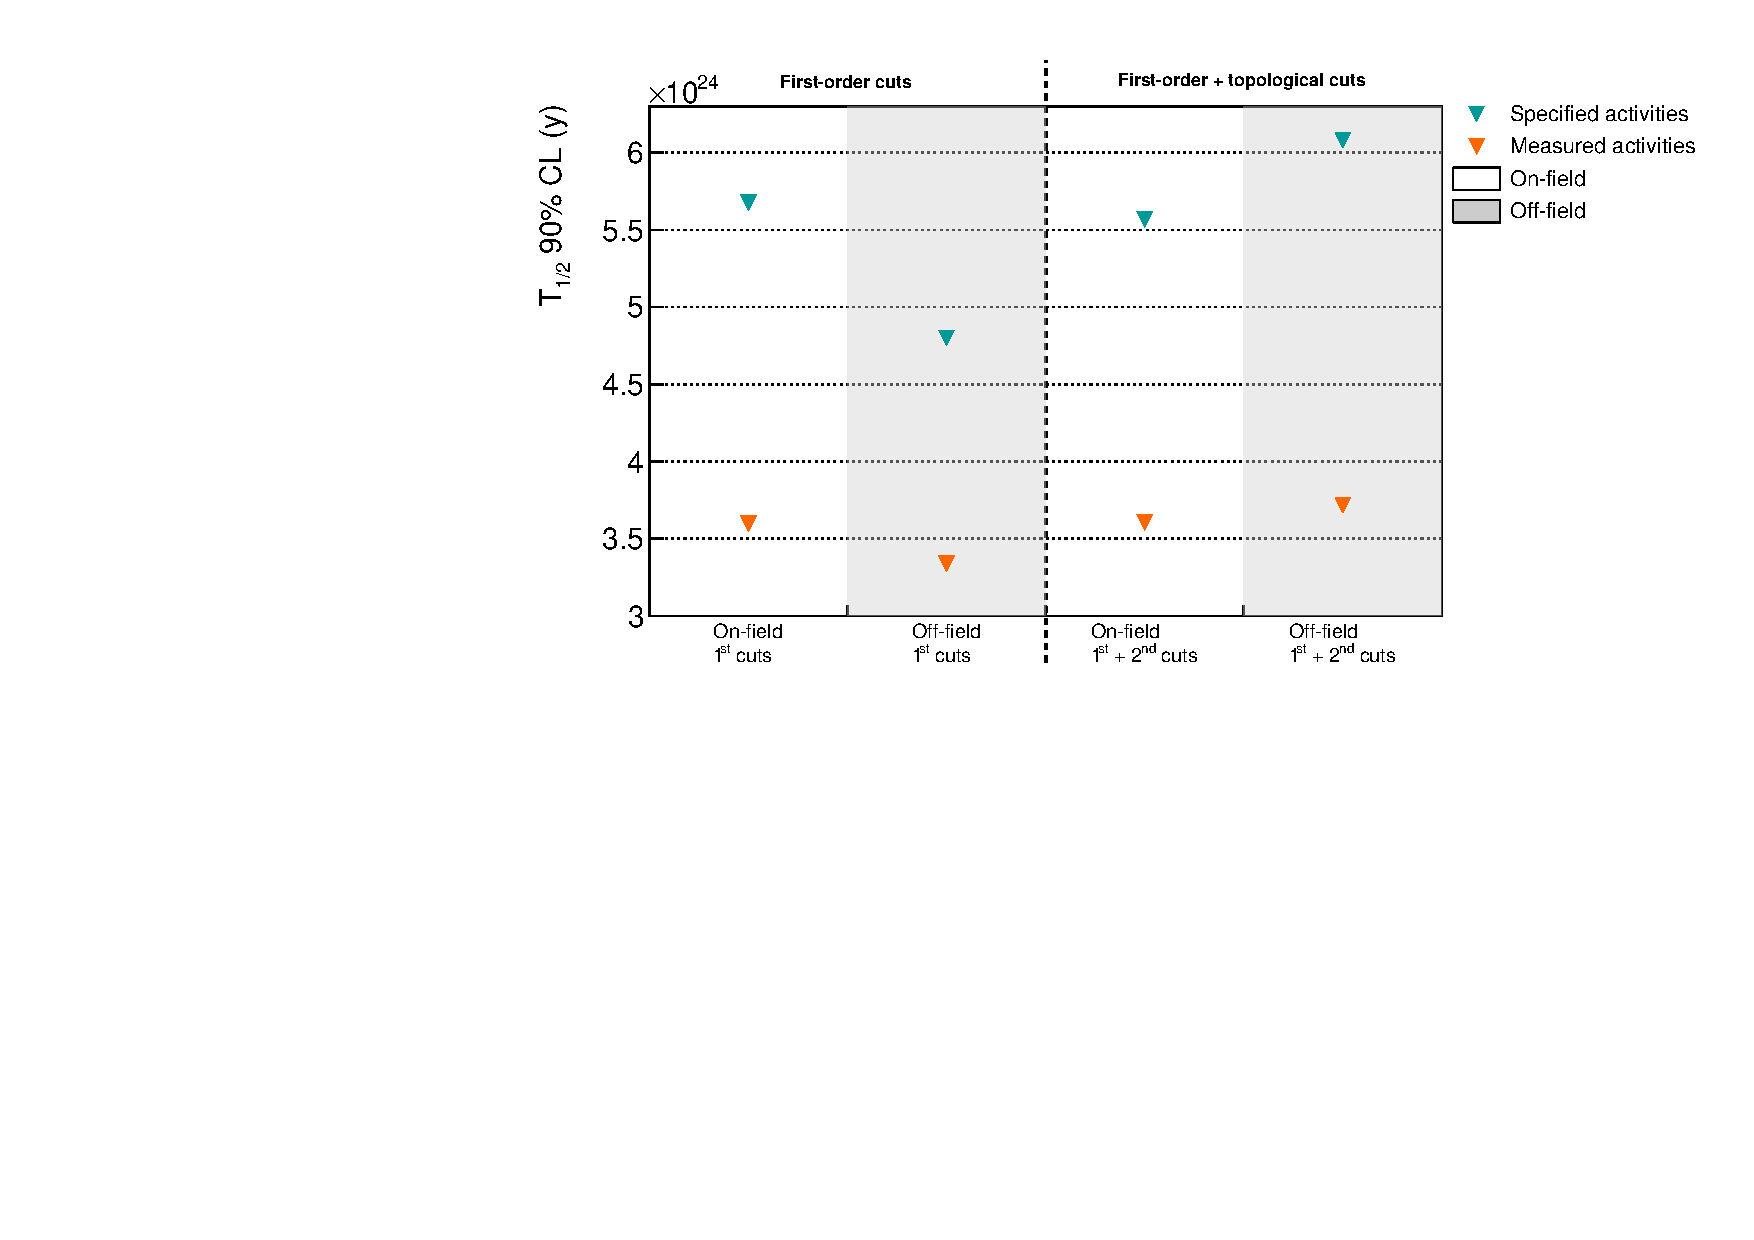
\includegraphics[width=1.1\textwidth]{Sensitivity/fig_sensitivity/contamination_Se_w_woB.pdf}
  \caption{$\Tbeta$ ($90$\% CL) considering various conditions: on- and off-field (white and grey stripes), first-order and addition of topological cut-offs (left/right parts of the panel), specified and measured activities (blue and orange triangle markers).
    The measured activities are $\mathcal{A}^{\text{Tl}}=54~\mu$Bq/kg, $\mathcal{A}^{\text{Bi}}=290~\mu$Bq/kg and $\mathcal{A}^{\text{Rn}} = 0.15$~mBq/m$^{3}$.
    \label{fig:sensitivity_B}}
\end{figure}
The left part of the panel gives information on the evolution of sensitivity, when only the first-order cut-offs are applied.
We come back to the conclusions given above: when the magnetic field is switched-off, we lose sensitivity, regardless of the level of contamination considered.
On the right side of the figure, we present the results when the topological cuts are applied.
For the on-field case, the addition of these selections have almost no effect on the sensitivity, as concluded in sub-section~\ref{subsec:opti_ev_selection}.
However, as predicted, we are beginning to see the usefulness of these selections in the off-field case, as a higher number of \Tl\ and \Rn\ events passed the first-order selections.
For instance, for the specification case, $\Tbeta$ goes from $4.8\times 10^{24}\,\text{y}$ to $6.1\times 10^{24}\,\text{y}$, an improvement of~$\sim~30\%$.

In Tab.~\ref{tab:Nexp_noField} are presented the expected number of background events in the ROI for the off-field condition, before and after application of topological cut-offs, for the specified and measured activities (taking into account the upper limit for the \Bi\ contamination).
\begin{table}[h!]
  \centering
  \begin{tabular}{|c|c|c|c|c|}
    \hline
    Activity & \multicolumn{2}{c|}{Specified} & \multicolumn{2}{c|}{Measured (w/ \Bi)} \\
    \hline
    Cut-off & First-order & Topological & First-order & Topological  \\
    ROI (MeV) & [$2.75$;$3.2$] & [$2.7$;$3.2$] & [$2.65$;$2.9$] & [$2.7$;$2.9$] \\
    \hline\hline
    $\epsilon_{0\nu}$ & $12.4$\% & $15.7$\% & $19.1$\% & $14.8$\% \\
    \hdashline
    $\twonu$  & $0.0353$ & $0.453$ & $1.56$ & $0.440$ \\
    \Tl  & $0.0600$ & $0.0506$ & $1.01$ & $0.613$ \\
    \Bi  & $0.0452$ & $0.0706$ & $2.94$ & $1.84$ \\
    \Rn  & $0.553$ & $0.0894$ & $1.42$ & $0.0689$ \\
    Total & $0.693$ & $0.664$ & $6.93$ & $2.96$ \\
    \hline
  \end{tabular}
  \caption{Selection efficiency of $\zeronu$ events and expected number of backgrounds events in the optimised ROI, for the exposure of the SuperNEMO demonstrator (17.5 kg.y), with off-field condition.
    Specified and measured (with \Bi) activities are considered.
    Topological cut-offs are optimised: \Pint$>1$\% and $|\Delta Z|<80$mm (specified activities),  \Pint$>5$\% and $|\Delta Z|<80$mm (measured activities)
    \label{tab:Nexp_noField}}
\end{table}
This selection allows to reject mainly \Rn\ background.
Prior to the application of the topological cuts, the relatively large number of Radon events ($0.553$) prevented the value of the lower limit of ROI from lowering.
Once the topological cuts have drastically reduced Radon, the lower limit decreases, thus increasing the $\twonu$.
Fortunately, it is also accompanied by an increase in the selection of $\zeronu$ events.
Finally, even if the absence of the magnetic field has the effect of reducing the sensitivity to the $\zeronu$ decay, topological cuts allow this effect to be compensated for, making it possible to reach higher values of $\Tbeta$.


%% \begin{itemize}
%% \item pour la variation de la ROI dans la figure comparative des différents level en contaminations : la ROI bouge pour les cas measured. C'est étonnant à premièer vue car ça ne paraît pas optimal et ça rajoute du Bi. Mais en fait si on regarde  les biplots de sensibilité, on a des fluctuations. Mais ce ne sont pas de grosses fluctuations, ce qui est aussi rassurant car ça veut dire qu'on n'est pas trop sensible aux variations de Emin/Emax (même si j'ai dit qu'on y était pas mal sensible -> à regarder)
%% \end{itemize}

\subsection{Influence of the magnetic field on optical modules and reconstruction efficiency}

In the previous sub-section, a comparative study has been led to evaluate the influence of the presence of a magnetic field on the event selection, and thus on the final sensitivity.
However, as things stand now, some features of the demonstrator are not yet implemented in the simulation software, and could have a great impact on the results presented above.
In particular, studies have been led by the collaboration to evaluate the influence a $25$~Gauss magnetic field on the optical modules, as well as on the event reconstruction~\cite{CalvezThesis,internal:magnetic_field}.

SuperNEMO PMTs are protected from the external magnetic field by individual iron shields.
Unfortunately, the latter do not perfectly protect the PMTs, and a residual magnetic field is measured inside the shieldings, leading to losses in charge collected by PMTs close to $8\%$.
This study also revealed the energy resolution would be worsened with a relative decrease of $3\%$ of the initial value of $8\%$ at $1$~MeV.
Moreover, the PMTs shieldings could themselves severely impact the shape of the field lines, as well as its intensity.
In fact, with a $25$ Gauss magnetic field generated by the copper coil, the magnetic shields are responsible for the field strength decreasing, and barely $10$ G is expected near the source foils.
Worse, the magnetic field strength decreases very quickly as we get closer to the calorimeter walls, where nearly $0~$G could be expected.
The reconstruction efficiency could therefore be greatly impacted:
the magnetic field intensity varying from the source foils to the calorimeter wall, electrons trajectory curvatures are not constant, and the track-fitting algorithm is less performing.
An incorrect description of the distribution of the magnetic field would more strongly impact low-energy electrons.

In the light of these conclusions, it could be interesting to study the evolution of the sensitivity, considering field simulations with more realistic variations inside the detector.

%% Despite the fact that magnetic shields were designed and installed to protect the PMTs, this field can have a great impact on the calorimeter detection efficiency, and thus could degrade the detector's sensitivity to the $\zeronu$ decay.

\subsection{Simulations with a non-uniform magnetic field}
\label{subsec:mapped_field}

Simulations with a $25$~Gauss \emph{mapped} magnetic field have been performed, taking into account more realistic variations of the field inside the detector~\cite{docdb:map_magnetic_field2015}.
In this condition, the fitting algorithm follows the same steps as for on-field: a helix and linear fit are performed for each simulated event, and the most accurate is selected.
Unfortunately, Radon isotope decays could not be simulated with this magnetic field configuration.
Indeed, as it is present in the entire wire chamber, simulations would have required too many additional storing resources.
Thus, strong conclusions on the sensitivity can't be given.
However, it is possible to assess the selection efficiencies of the different processes, and then get an idea of the influence of realistic variations of the field on the final results.
%% Fig.~\ref{} displays
%% \begin{figure}[h!]
%%   \centering
%%   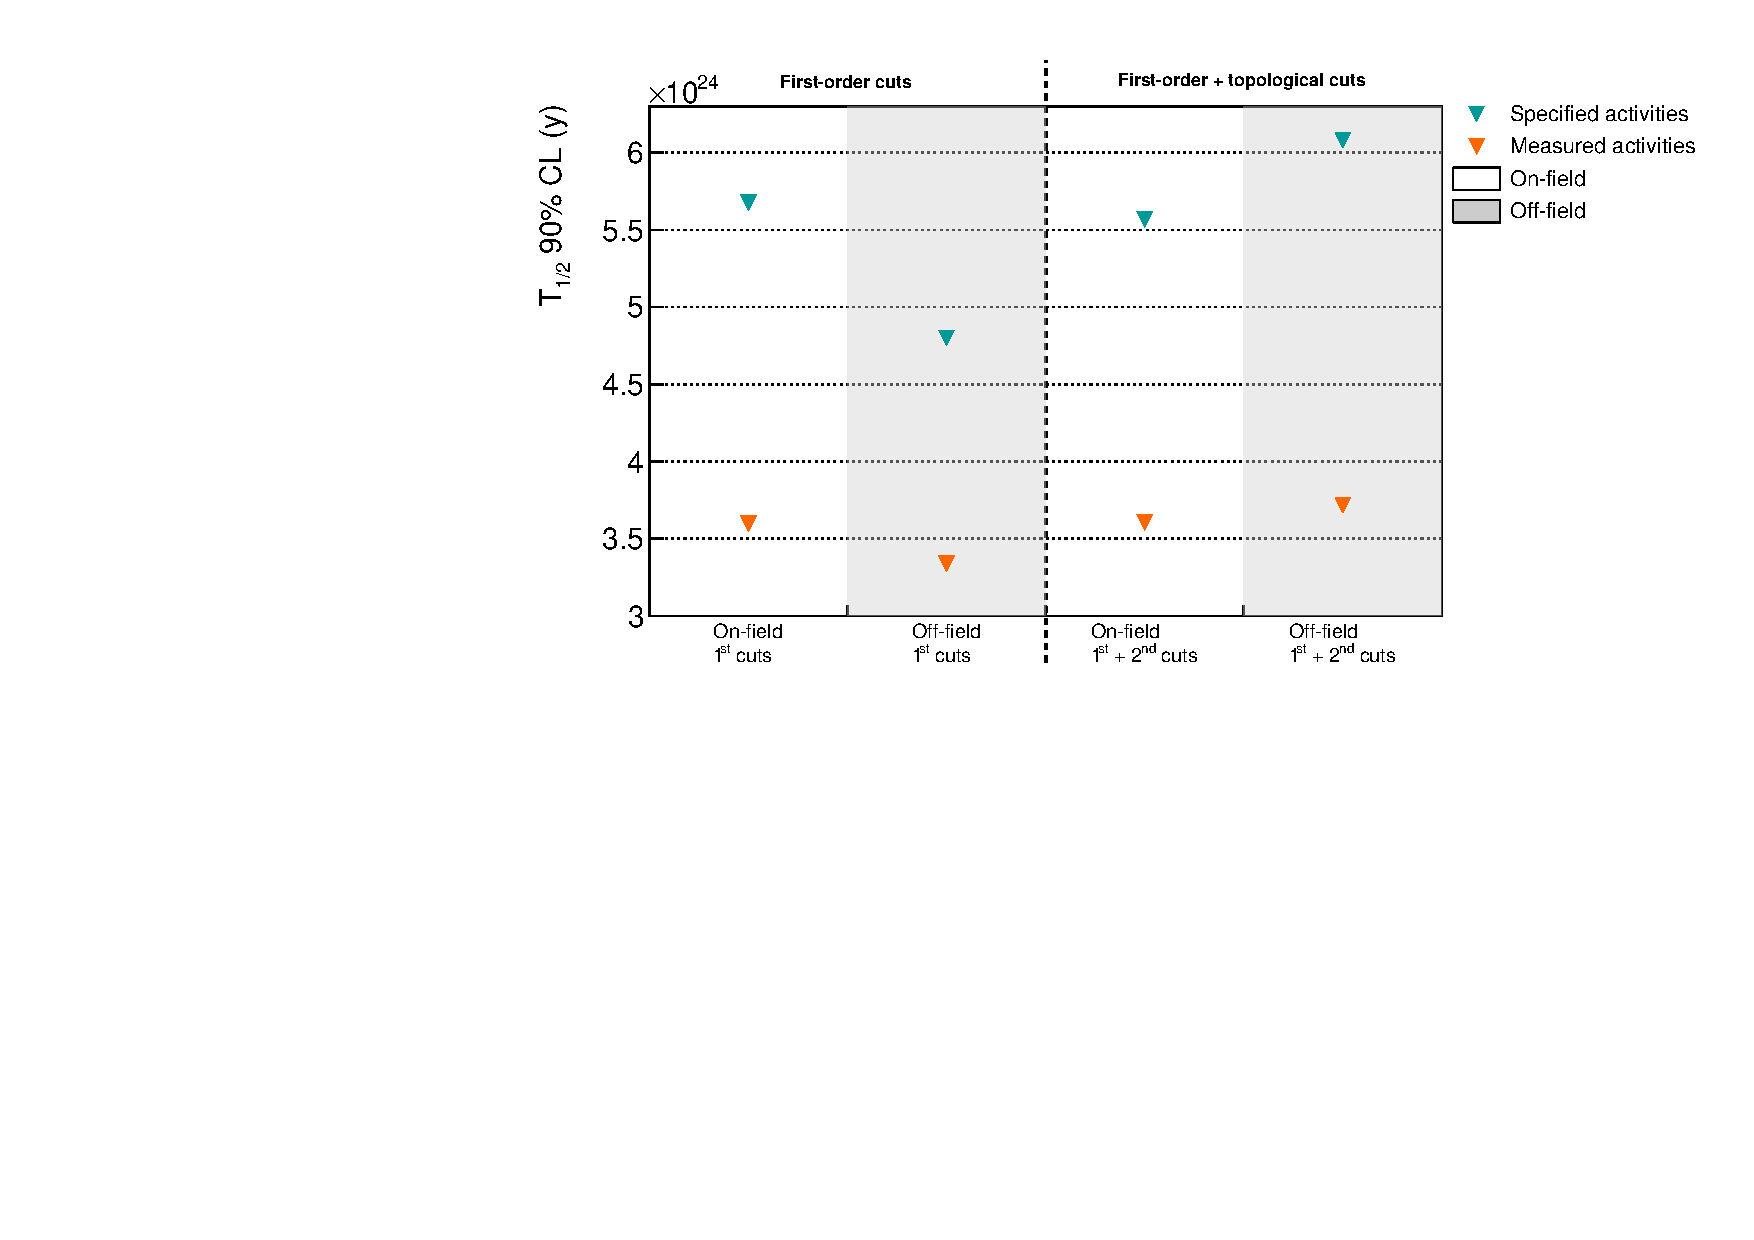
\includegraphics[width=1.1\textwidth]{Sensitivity/fig_sensitivity/contamination_Se_w_woB.pdf}
%%   \caption{Best limit set on $\zeronu$ half-life (top pad), and the corresponding ROI (bottom pad), as a function of the contamination level considered, for both on-field and off-field cases.
%%     \label{fig:}}
%% \end{figure}
Tab.~\ref{tab:mapped_eff} compares the selection efficiencies, for the three field cases (uniform on-field, mapped field and off-field), in the total energy range [$0$;$4$]~MeV.
\begin{table}[h!]
  \centering
  \begin{tabular}{|c|c|c|c|}
    \hline
    Field & On & Off & Mapped  \\
    \Pint & \Pint$>4$\% & \Pint$>1$\% & \Pint$>4$\% \\
    \hline\hline
    $\zeronu$ & $24.7$ & $29.3$ & $19.1$ \\
    $\twonu$ & $8.21$ & $9.93$ & $6.39$ \\
    \Tl & $0.0846$ & $0.140$ & $0.0774$ \\
    \Bi & $0.144$ & $0.211$ & $0.125$ \\
    \hline
  \end{tabular}
  \caption{Signal and background selection efficiencies of on-field, off-field and mapped-field cases, in the energy range [$0$;$4$]~MeV.
    The first-order and optimised topological cut-offs have been applied.
    Especially, for all field conditions, $|\Delta~Z|<80$~mm.
  \label{tab:mapped_eff}}
\end{table}
The mapped field case has lower selection efficiencies, compared with uniform field simulations.
As announced in the previous sub-section, the magnetic shields distort the field intensity across the detector.
Therefore, the fitting algorithm is less efficient in identifying particles with a negative curvature inside the tracker, hence the number of selected $2e$ topologies is decreased.

Tab.~\ref{tab:eff_mapped_ROI} presents the expected number of background events in the energy range [$2.7$;$3.2$]~MeV, for simulations using the realistic mapped field.
\begin{table}[h!]
  \centering
  \begin{tabular}{|c|c|}
    \hline
     & Mapped field  \\
    \hline\hline
    $\epsilon_{0\nu}$ & $10.4$\%  \\
    \hdashline
    $\twonu$  & $0.245$  \\
    \Tl  & $0.0279$  \\
    \Bi  & $0.0535$  \\
    Total & $0.326$ \\
    \hline
  \end{tabular}
  \caption{Selection efficiency of $\zeronu$ events and expected number of backgrounds events in the [$2.7$;$3.2$]~MeV optimised ROI, for the exposure of the SuperNEMO demonstrator (17.5 kg.y), for mapped field simulations.
    The specified background activities are considered.
    First-order and optimised topological cuts have been applied (\Pint$>4$\% and $|\Delta~Z|<80$~mm).
    \label{tab:eff_mapped_ROI}}
\end{table}
As expected, the $\zeronu$ selection efficiency is drastically decreased compared with the on-field case, as well as the expected number of background events.
As explained above, the selection on track curvature is still applied in this case, and the non-uniform magnetic field causes deviations in the particles trajectory, which are therefore more difficult to identify as electrons.
Even if Radon simulation with such field conditions are unavailable, it is interesting to provide an order of magnitude of the $\Tbeta$ limit set with these realistic variations of the field.
To do so, we extrapolate the expected number of Radon events in the [$2.7$;$3.2$]~MeV energy range, from the \Bi\ one.
Indeed, we postulate the ratio between these two numbers remain a constant, and the on-field simulations give $N_{\text{Bi}}/N_{\text{Rn}}\sim5$.
Taking this into consideration, a limit of $\Tbeta~>~4\times~10^{24}$~y ($90$~\% CL) would be reached with the demonstrator, a $\sim 30$~\% decrease compared with the non-realistic uniform case.
This approximation should be examined with caution, however, as magnetic field conditions can greatly influence the selection of Radon and Bismuth events.
To be specific, we have seen in Sec.~\ref{subsec:impact_field} that between off-field and on-field conditions, the Radon and Bismuth efficiencies varied differently.
So, to ensure that our approximation is valid, a more proper study would have to be made.
In particular, it would be necessary to study how events where the two electrons are emitted back to back from a wire of the tracker when the field is no longer uniform are treated.

\section{Searching for the \Nd\ $\zeronu$ decay}
\label{sec:Nd}

This study was conducted jointly with the PhD student Axel Pin, from CENBG~\cite{AxelThesis}.
Although we both worked on the whole of the analysis, I presented in detail, in the previous sections, the results regarding the influence of the magnetic field.
Meanwhile, Axel Pin presents the possibility of changing the Selenium material by other $\beta\beta$ isotopes.
Indeed, on the model of the NEMO-$3$ detector, which housed, among others, $6.914$~kg of \Mo\ and $0.932$~kg of \Se, the SuperNEMO detector possesses the technical possibility of exchanging the source material and study several $\beta\beta$ isotopes.
Notably, in the case SuperNEMO demonstrates the feasibility of a large-scale tracko-calo experiment, it would be natural to  evaluate the sensitivity of SuperNEMO to the $\zeronu$ decay of other isotopes than \Se.

\subsection{Searching for the $\zeronu$ of other isotopes}

One of the distinctive features of NEMO detectors is the gaseous detector, designed to track charged particles.
Unluckily, this advantage is also a great inconvenience when it comes to Radon contamination.
Indeed, Radon enters by diffusion or emanates from the detector materials.
It is then interesting to consider $\beta\beta$ candidates with an energy transition value above the $Q_{\beta}=3.27$~MeV of 214Bi, a Radon daughter.
Another useful criterion is the natural isotopic abundance: typically, considering only isotopic abundances greater than 2\% is a reliable basis when selecting potential $\beta\beta$ emitters.
Two nuclei satisfy these two criteria: $^{96}$Zr and \Nd\ (with respective $\Qbb$ values of $3.35$ and $3.36$~MeV, and respective isotopic abundances of $2.8$ and $5.6$~\%~\cite{art:atomic_mass}).
%% Given the availability of \Mo, much effort has been focused by the NEMO-$3$ collaboration on this isotope (it had already been studied by the NEMO-$2$ prototype~\cite{art:NEMO2}).
As the \Nd\ isotope has the highest $\Qbb$ value, the current section focuses on evaluating the SuperNEMO sensitivity to the $\zeronu$ decay of this isotope, supposing we have several kg at our disposal.
Moreover, the \Nd\ has a more favourable phase space than the \Se, on which the half-life limit directly depends.

\subsection{Sensitivity to the $\zeronu$ of \Nd}

Until recently, Neodymium was not enrichable in large quantities.
Recent developments have resulted in the production of several grams of enriched Neodymium, making this $\beta\beta$ isotope interesting for the search for $\zeronu$.
Thanks to that, NEMO-$3$ had available $36.6$~g of \Nd\ which were recovered by the collaboration, for a possible reuse for SuperNEMO.
The best limit for the search for neutrinoless double $\beta$ decay of \Nd\ was reached by the NEMO-$3$ detector with $5.25$~years of data acquisition.
The detector achieved $\Tbeta~>~2.0\times~10^{23}$~y~($90$~\%~CL), corresponding to a range on the effective neutrino mass of $\langle\mbb\rangle~<~[1.6-5.3]$~eV.
The collaboration also measured the $\twonu$ half-life, with $\Ttwonu~=~$[$9.34~\pm~0.22$~(stat.)~$\pm~^{0.62}_{0.60}$~(syst.)]$\times~10^{18}$~y~\cite{art:NEMO3_Nd}.

We wish to determine the limit on the $\zeronu$ of the \Nd\ that could be reached with the SuperNEMO demonstrator, with an exposure of $17.5$~kg.y.
We lead this study considering the activities specified for the \Se\ sources are reached.
We use simulations with the $25$~Gauss uniform magnetic field.
Fig.~\ref{fig:energy_Nd} depicts the normalised energy distributions for the $2e$ topologies selected after application of first-order and topological selections.
\begin{figure}[h!]
  \centering
  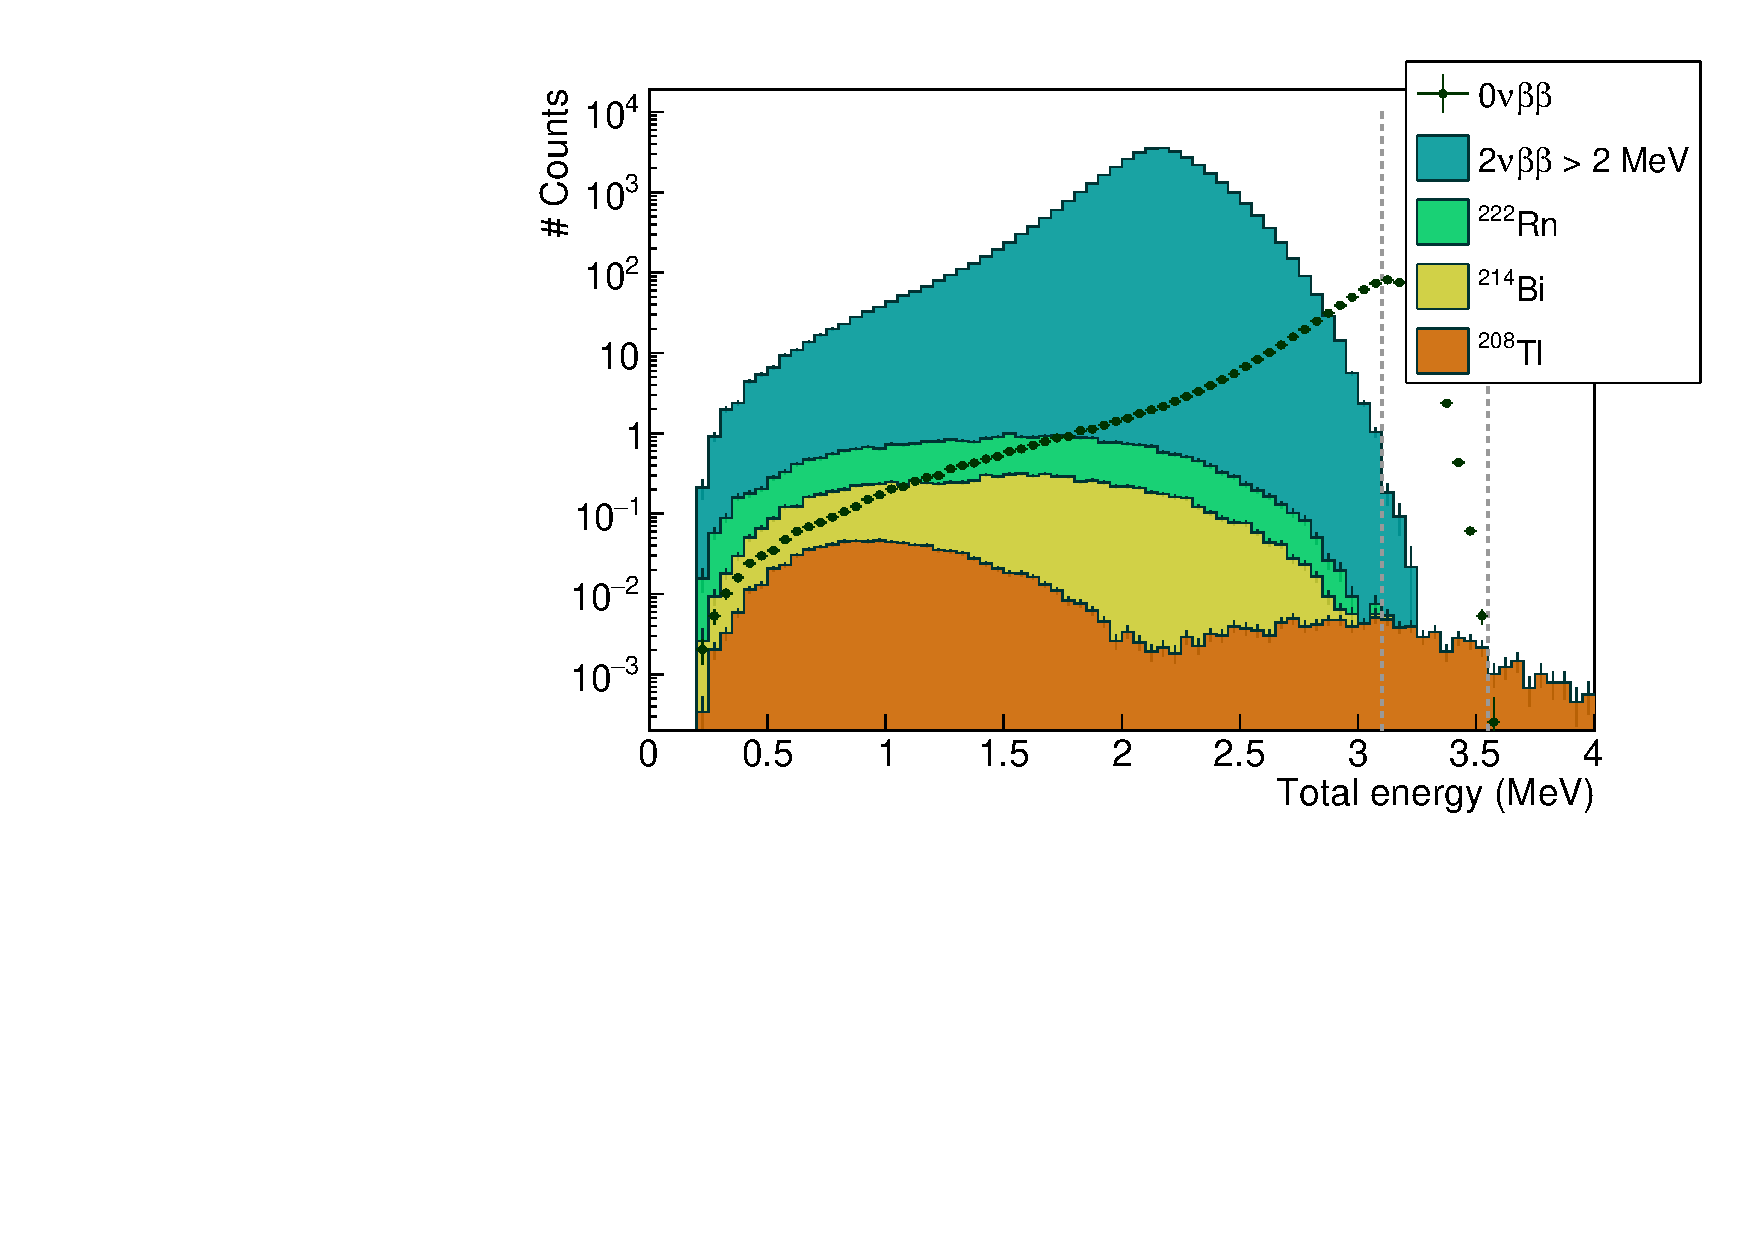
\includegraphics[width=0.8\textwidth]{Sensitivity/fig_sensitivity/energy_spectrum_with_B_150Nd.pdf}
  \caption{Total energy spectra for the $\zeronu$ signal and main backgrounds, for \Nd\ sources and for a $17.5$~kg.y exposure.
    The $\twonu$ spectrum is normalised to $\Ttwonu~=~9.34\times~10^{18}$~y, and \Tl, \Bi\ and \Rn\ backgrounds are normalised to the nominal activities.
    The amplitude of the $\zeronu$ is arbitrarily set at the limit obtained with NEMO-$3$ $\Tbeta~=~2.0\times~10^{23}$~y.
    First-order and optimised topological cuts have been applied.
    The ROI of [$3.1$;$3.55$]~MeV is depicted by to vertical dashed lines.
    \label{fig:energy_Nd}}
\end{figure}
Signal and background selection efficiencies for \Nd\ sources, in the total energy range, are given in Tab.~\ref{tab:energy_spect_Nd}.
\begin{table}[h!]
  \centering
  \begin{tabular}{|c|c|c|}
    \hline
    Isotope & Selenium & Neodymium \\
    \hline\hline
    $\zeronu$  & $25.8$ & $25.5$ \\
    $\twonu$  & $8.21$ & $8.11$ \\
    \Tl  & $0.0846$ & $0.0749$ \\
    \Bi  & $0.144$ & $0.138$ \\
    \Rn  & $5.34\times 10^{-3}$ & $5.34\times 10^{-3}$ \\
    \hline
  \end{tabular}
  \caption{Selection efficiencies in the full energy range [$0$;$4$]~MeV, for \Se\ and \Nd\ sources.
    First-order and optimised topological cuts have been applied.
    \label{tab:energy_spect_Nd}}
\end{table}
The selection efficiencies of backgrounds are lower for \Nd\ sources than for \Se\ sources.
In both cases, for the total energy range the background contribution is dominated by the $\twonu$ decay.
This is caused by the more elevated number of protons in the Neodymium nucleus which induces a stronger Coulombian effect.
Indeed, the more the $\beta\beta$ emitter has a high atomic number $Z$, the more the electrons emitted from inside the source (or passing through it) are likely to interact electromagnetically with it.
Despite this, for reasons of limited storage resources, we choose to consider this effect to be negligible for events outside the source, such as Bismuth disintegrations (from Radon) from the tracker wires.
Therefore, we choose to use the Radon simulations already generated for the \Se\ sources study.
Clearly, further study would be required to ensure that this consideration is reasonable.

In Tab.~\ref{tab:Nexp_Nd_ROI} we give the expected number of background events in the optimised ROI [$3.1$;$3.55$]~MeV.
\begin{table}[h!]
  \centering
  \begin{tabular}{|c|c|c|}
    \hline
    Isotope & Selenium & Neodymium \\
    ROI & [$2.7$;$3.15$]~MeV & [$3.1$;$3.55$]~MeV \\
    \hline\hline
    $\epsilon_{0\nu}$ & $14.4$\% & $10.3$\% \\
    \hdashline
    $\twonu$  & $0.39$ & $0.28$ \\
    \Tl  & $0.044$ & $0.029$ \\
    \Bi  & $0.053$ & $5.6\times 10^{-4}$ \\
    \Rn  & $0.20$ & $0.0$ \\
    Total & $0.687$ & $0.309$ \\
    \hline
  \end{tabular}
  \caption{Selection efficiency of $\zeronu$ events and expected number of backgrounds events in the optimised ROI, for the exposure of the SuperNEMO demonstrator (17.5 kg.y), for \Se\ and \Nd\ sources.
    The specified background activities are considered.
    First-order and optimised topological cuts have been applied.
    \label{tab:Nexp_Nd_ROI}}
\end{table}
The selection efficiency of the $\zeronu$ decay in this energy range is also given.
Although the $\twonu$ half-life of the \Nd\ is lower than that of the \Se\ by a factor $\sim~10$, the number of $\twonu$ events in the ROI remains low.
Indeed, thanks to the Coulombian effects described above, this process has a limited contribution at high energy.
The high energy of transition $\Qbb~=~3.36$~MeV of \Nd\ implies that the contributions of \Bi\ and \Rn\ are very small, or even zero.
The $\twonu$ and \Tl\ events are therefore the major contributors to the background.
Consequently, if the choice of changing the source material with \Nd\ isotope was made, it would be conceivable to release the specifications on \Bi\ and \Rn\ backgrounds.

The SuperNEMO demonstrator, with $7$~kg of \Nd\ and $2.5$~years of data acquisition, would achieve a $\Tbeta~>~2.2\times~10^{24}$~y sensitivity, one order of magnitude higher than the best limit ever reached.
The corresponding limit on the effective neutrino mass is $\langle\mbb\rangle~=~[0.15-0.50]$~eV.
This is a better result than for \Se\ sources, as the \Nd\ has a more favourable space factor.


\section{The final detector sensitivity}

The ultimate goal of the SuperNEMO demonstrator is to show that the NEMO technology is scalable to probe unprecedented half-life on the $\zeronu$ decay.
The final detector would consist in building $20$ modules similar to the demonstrator.
In this context, we estimate the final detector sensitivity to the $\zeronu$ decay.

We suppose the specified activities of $\mathcal{A}^{\text{Tl}} = 2~\mu$Bq/kg, $\mathcal{A}^{\text{Bi}} = 10~\mu$Bq/kg and $\mathcal{A}^{\text{Rn}} = 0.15$ mBq/m$^{3}$ are reached.
The simulations with an uniform magnetic field are used.

Tab.~\ref{tab:Nexp_HN} shows the number of expected events in the optimised ROI for first-order and topological cut-offs.
\begin{table}[h!]
  \centering
  \begin{tabular}{|c|c|c|}
    \hline
    Cut & First-order & Topological  \\
    ROI & [$2.75$;$2.95$] MeV & [$2.75$;$3.1$] MeV \\
    \hline\hline
    $\epsilon_{0\nu}$ & $11.3$\% & $10.7$\%  \\
    \hdashline
    $\twonu$  & $3.48$ & $3.36$  \\
    \Tl  & $0.728$ & $0.756$  \\
    \Bi  & $0.945$ & $0.835$  \\
    \Rn  & $6.93$ & $2.16$  \\
    Total & $12.1$ & $7.11$ \\
    \hline
  \end{tabular}
  \caption{Selection efficiency of $\zeronu$ events and expected number of backgrounds events in the optimised ROI, for the exposure of the SuperNEMO final detector ($500$~kg.y).
    The specified background activities are considered.
    The topological selections have been optimised: \Pint$>4$\% and $|\Delta~Z|<80$~mm.
    \label{tab:Nexp_HN}}
\end{table}
The total expected number of background events is high enough for the optimised cut-offs to be worth it, with \Pint\ $>~4~\%$ and $|\Delta~Z|~<80$~mm (similarly for $|\Delta~Y|$).
They allow primarily to reduce the Radon background by a factor $3$.
Due to the optimisation of the ROI, especially to the raising of the upper bound, the \Tl\ background is a little increased, without important consequences, as the $\twonu$ and \Rn\ dominate the total number of background in this energy range.

With an exposure of $500$~kg.y, the SuperNEMO final detector should reach a sensitivity of $\Tbeta~>~5.4\times~10^{25}$~y, with \Se\ sources, corresponding to $\langle\mbb\rangle~=~[0.079-0.15]$~eV.
By comparison, with the same exposure and background specifications but with \Nd\ sources, the final detector would achieve a sensitivity of $\Tbeta~>~2.2\times~10^{25}$~y, in the [$3.1$;$3.75$]~MeV ROI, corresponding to $\langle\mbb\rangle~=~[0.046-0.15]$~eV.


\section{Conclusion}

Latest measurements of source activities by BiPo-$3$ show that the specified background level for Thallium isotope is not reached, although it is improved on average by a factor $2$, compared to NEMO-$3$.
An upper limit is given for the internal Bismuth isotope activity.
In addition, not all sources were measured and a precise measurement is expected to be provide by the SuperNEMO demontrator when data acquisition will begin.
C-sections measurements with a concentration line showed the Radon targeted activity can be achieved for the demonstrator, with an gas flow rate of $2$~m$^{3}$/h inside the chamber.
Topological selections, designed to reject non-internal and non-simultaneous $2e$ events, have been optimised, and allowed to reduce the Radon background by a factor $3$ for the final demonstrator.
Assuming the target background activities are reached, the SuperNEMO demonstrator, running for two and half years with $7$~kg of \Se, would be able to a set a limit on the $\zeronu$ process $\Tbeta~>~5.4\times~10^{24}$~years, translating into a limit on the neutrino effective mass $\langle\mbb\rangle~<~[0.25-0.48]$~eV\footnote{The real mass of isotope is $6.23$~kg, then to achieve a $17.5$~kg.y exposure, the demonstrator should run a little more than two years and a half.}.
Taking into account the measured activities (with $290~\mu$Bq/kg of \Bi), the limit on $\Tbeta$ would be decreased by a factor $33$\% with $\Tbeta~>~3.6\times~10^{24}$~years ($\langle\mbb\rangle~<~[0.31-0.59]$~eV).
This limit could be enhanced by using a multivariate analysis, similarly to what is done in other double beta decay experiments, taking advantage of the several topological variables offered by SuperNEMO.

Recent studies have shown that the $25$~Gauss magnetic field would be distorted by detector materials, especially the calorimeter magnetic shields.
In this context, we studied the influence of this field on the demonstrator sensitivity.
Switching-off the field would enhance the expected number of $2e$ topologies, especially for background processes, and decrease the sensitivity.
This effect is compensated by applying optimised topological cut-offs which are useful with such a level of background.
Finally, without magnetic field, the SuperNEMO demonstrator would set a limit on the sensitivity of $\Tbeta~>~6.1\times~10^{24}$~years ($\langle\mbb\rangle~<~[0.24-0.46]$~eV), taking into account the specified activities, a $13$\% increase on $\Tbeta$ compared with the on-field case.
With the measured activities, $\Tbeta~>~3.7\times~10^{24}$~years ($\langle\mbb\rangle~<~[0.30-0.58]$~eV), an improvement of $3$\% compared with the on-field case.
Simulations with a mapped field have shown that the signal and background selection efficiencies would be degraded by a non-uniform, more realistic magnetic field.

Like its predecessor, the SuperNEMO demonstrator was designed to study several isotopes, such as the \Nd.
Assuming the target background activities are reached for \Nd\ sources, the SuperNEMO demonstrator would achieve a $\Tbeta~>~2.2\times~10^{24}$~years ($\langle\mbb\rangle~<~[0.15-0.51]$~eV).

Finally, assuming we reach the target background levels, the SuperNEMO final detector would achieve an unprecedented limit of $\Tbeta~>~5.4\times~10^{25}$~years for \Se\ sources, corresponding to $\langle\mbb\rangle~=~[0.079-0.15]$~eV.
For \Nd\ sources, the half-life $\Tbeta~>~2.4\times~10^{25}$~years would be reached.
This corresponds to $\langle\mbb\rangle~=~[0.046-0.15]$~eV, better than for \Se\ sources, thanks to its higher phase-space factor.

To go further in this study, the SuperNEMO collaboration would study the influence on the sensitivity of external backgrounds, coming from detector materials as well as the laboratory.
Also, more realistic performances of the detector, as well as field variations have to be implemented in the software for the simulations to reproduce more accurately the data.

As the \Tl\ background is higher than specified, and topological cut-offs are not strongly efficient to reduce its contribution, the next chapter focuses on setting up a specific technique to reject this internal background.
%% \begin{itemize}
%% \item Plot général récap tous résultats

%% \item manque de stat pour le neodyme car ROI haute E
%% \item légères diff avec résultats axel car légères diff dans sélections d'ev car utilisation PID

%% \item cellules tracker dead-> refaire analyse
%% \item delayed cells->improvement, cf NEMO 3
%% \end{itemize}

%% \begin{figure}[h!]
%%   \centering
%%   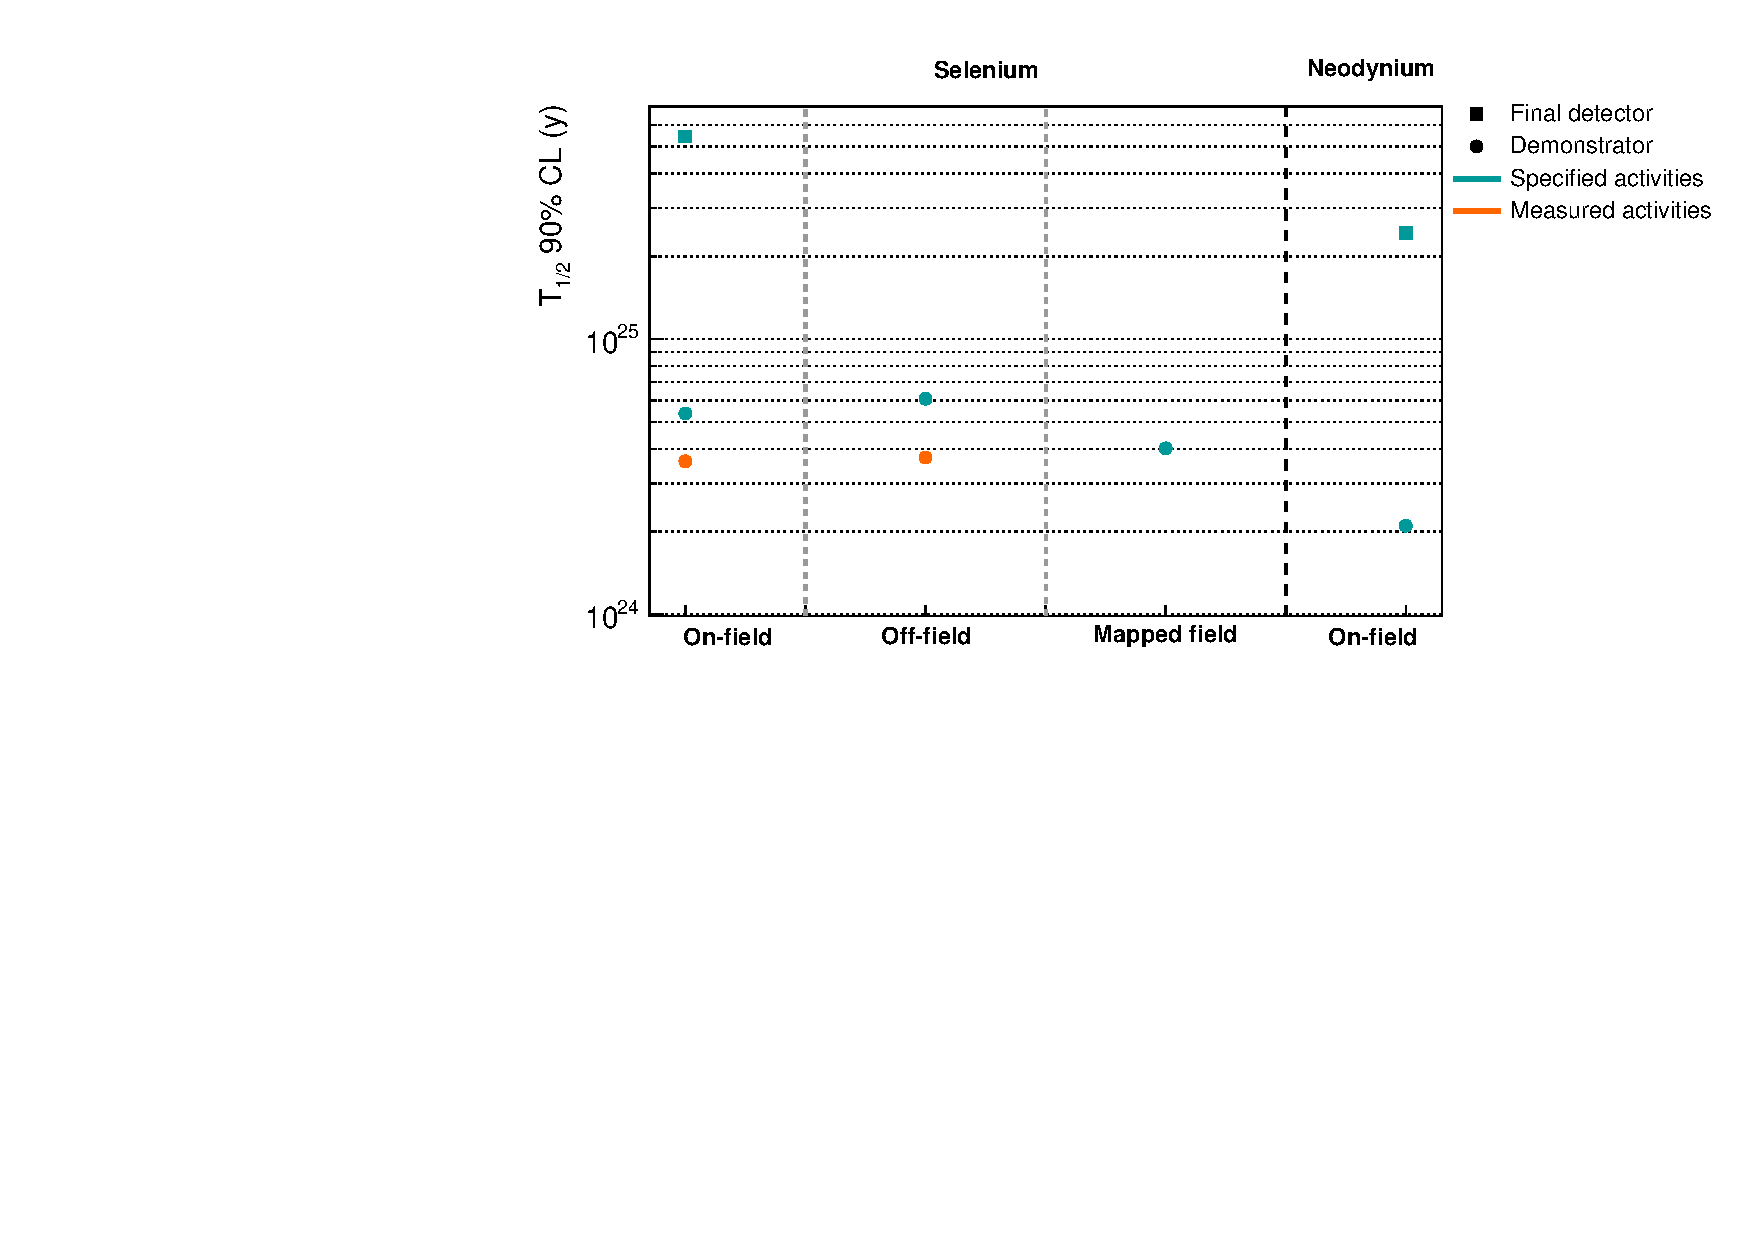
\includegraphics[width=1.1\textwidth]{Sensitivity/fig_sensitivity/final_t12.pdf}
%%   \caption{Summary of $\Tbeta$ $90$\% limits set.
%%     First-order and optimised topological cut-offs have been applied.
%%     Regions of interest have been optimised for each case.
%%     \label{fig:final_t12}}
%% \end{figure}
%% \begin{figure}[h!]
%%   \centering
%%   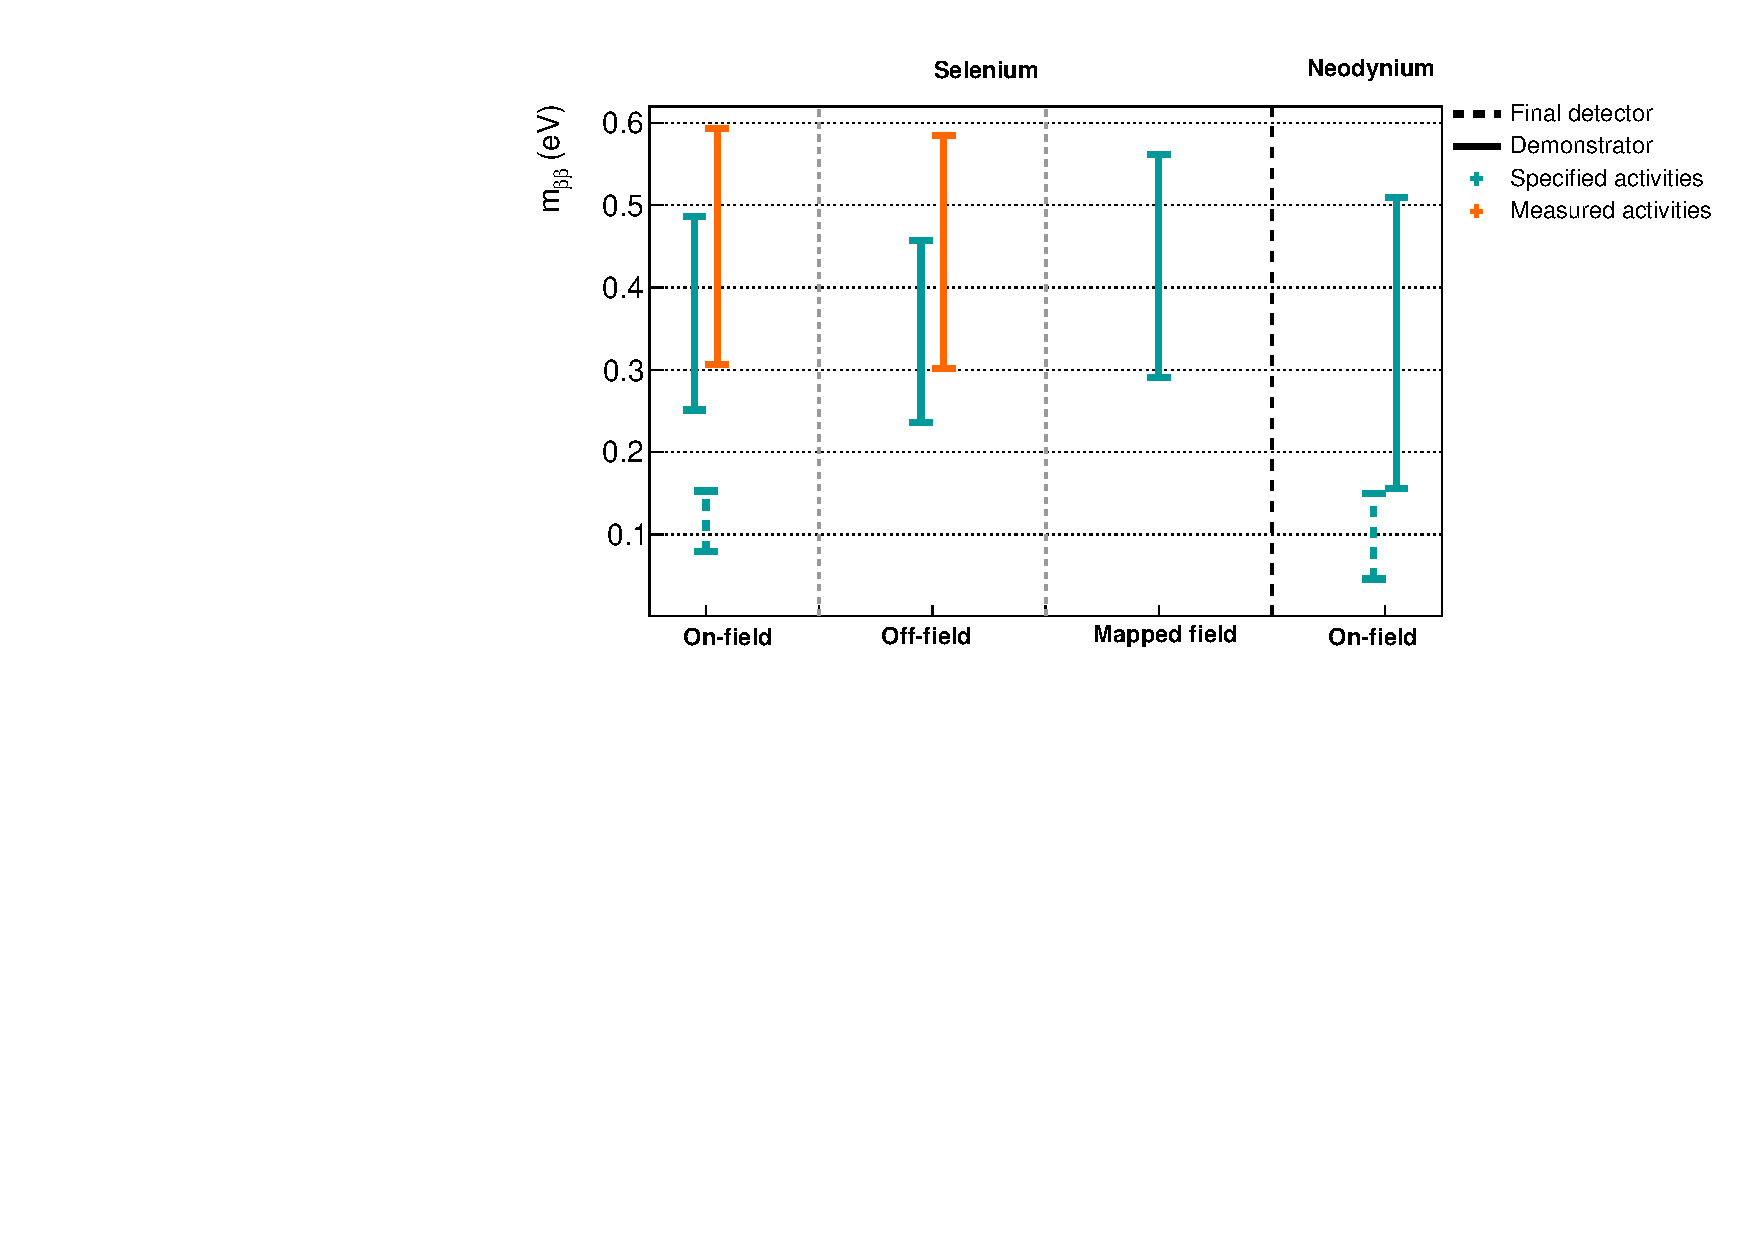
\includegraphics[width=1.1\textwidth]{Sensitivity/fig_sensitivity/final_mbb.pdf}
%%   \caption{Summary of $\mbb$ limits set.
%%     First-order and optimised topological cut-offs have been applied.
%%     Regions of interest have been optimised for each case.
%%     \label{fig:final_t12}}
%% \end{figure}

\begin{figure}[!h]
\centering
\begin{subfigure}[t]{1\textwidth}
  \centering
  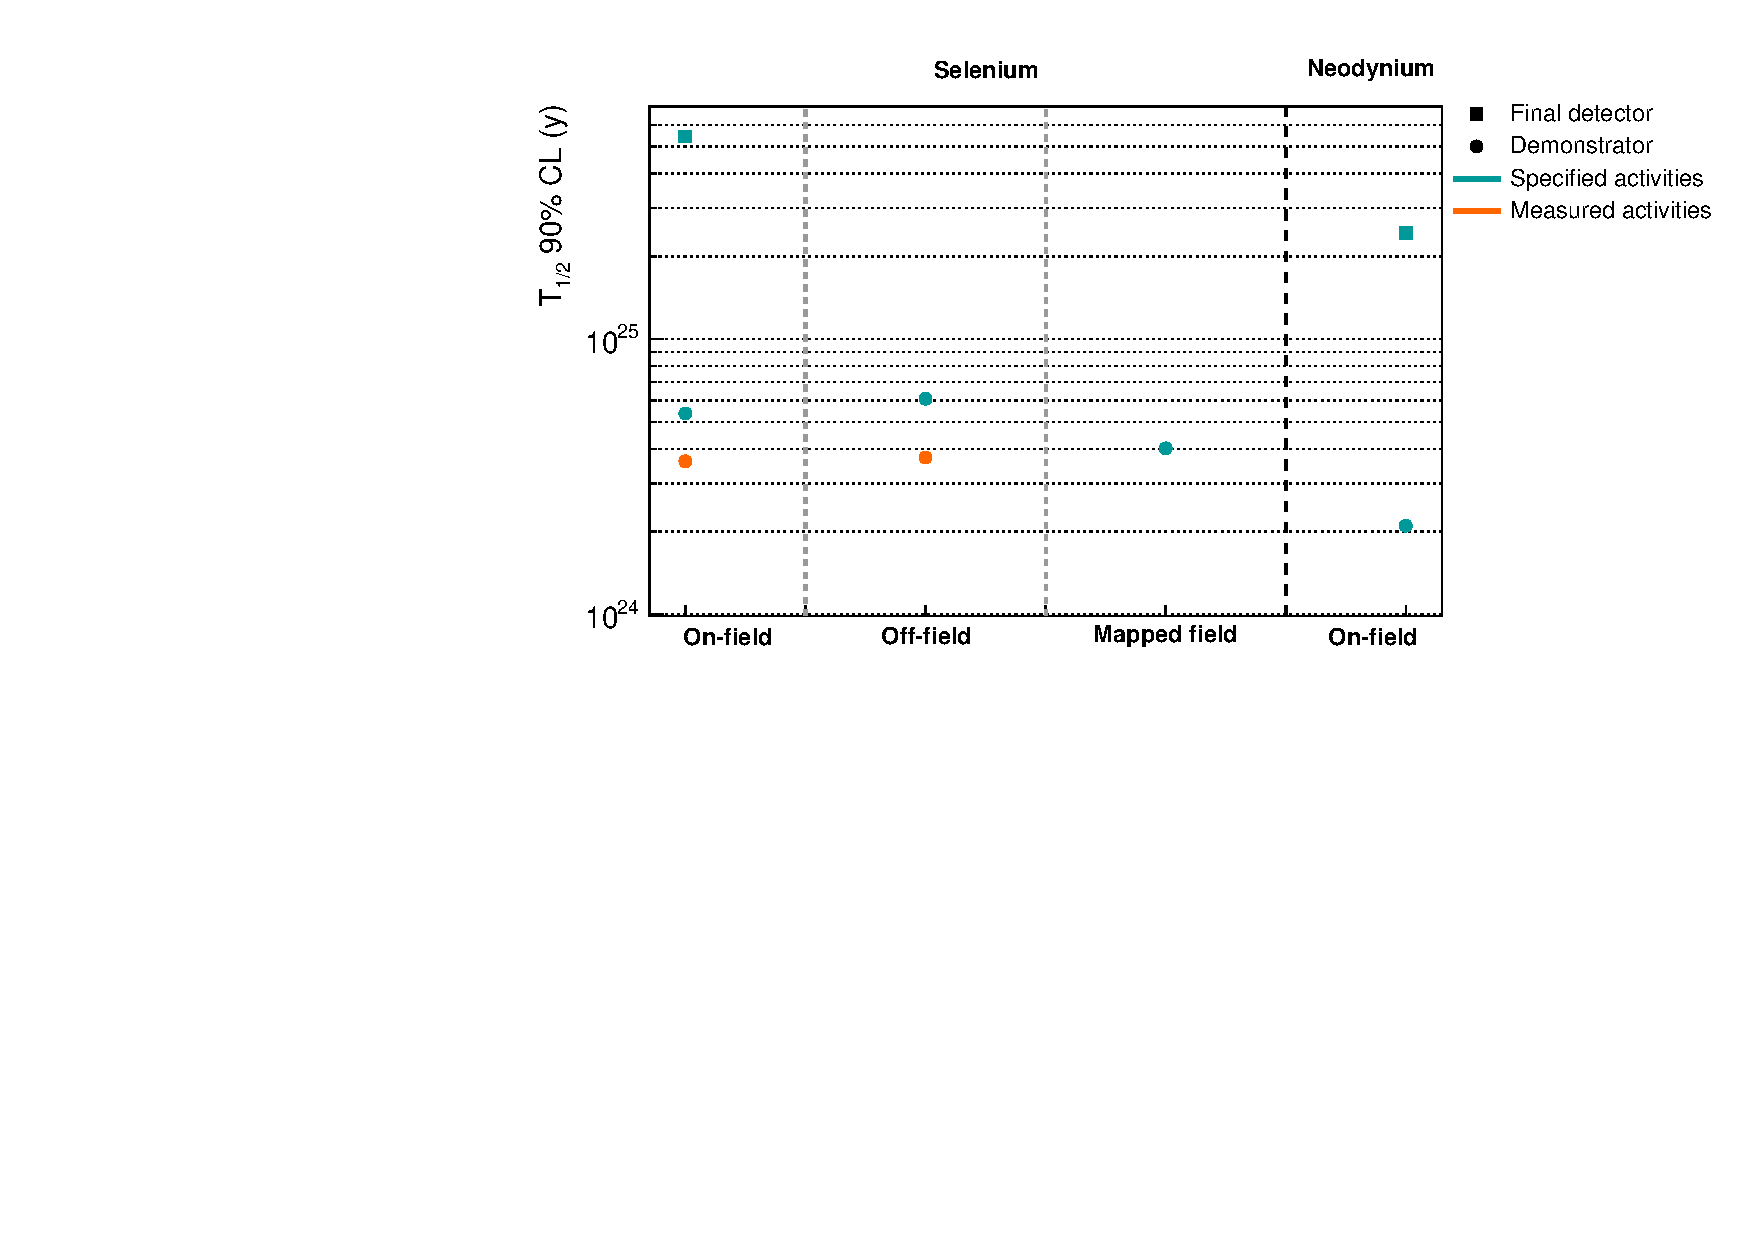
\includegraphics[width=1\textwidth]{Sensitivity/fig_sensitivity/final_t12.pdf}
  \captionsetup{justification=centering}
  \caption{$\Tbeta$ ($90$\% CL) limits.
    \label{subfig:summary_T12}}
\end{subfigure}
\vskip\baselineskip
\begin{subfigure}[t]{1\textwidth}
  \centering
  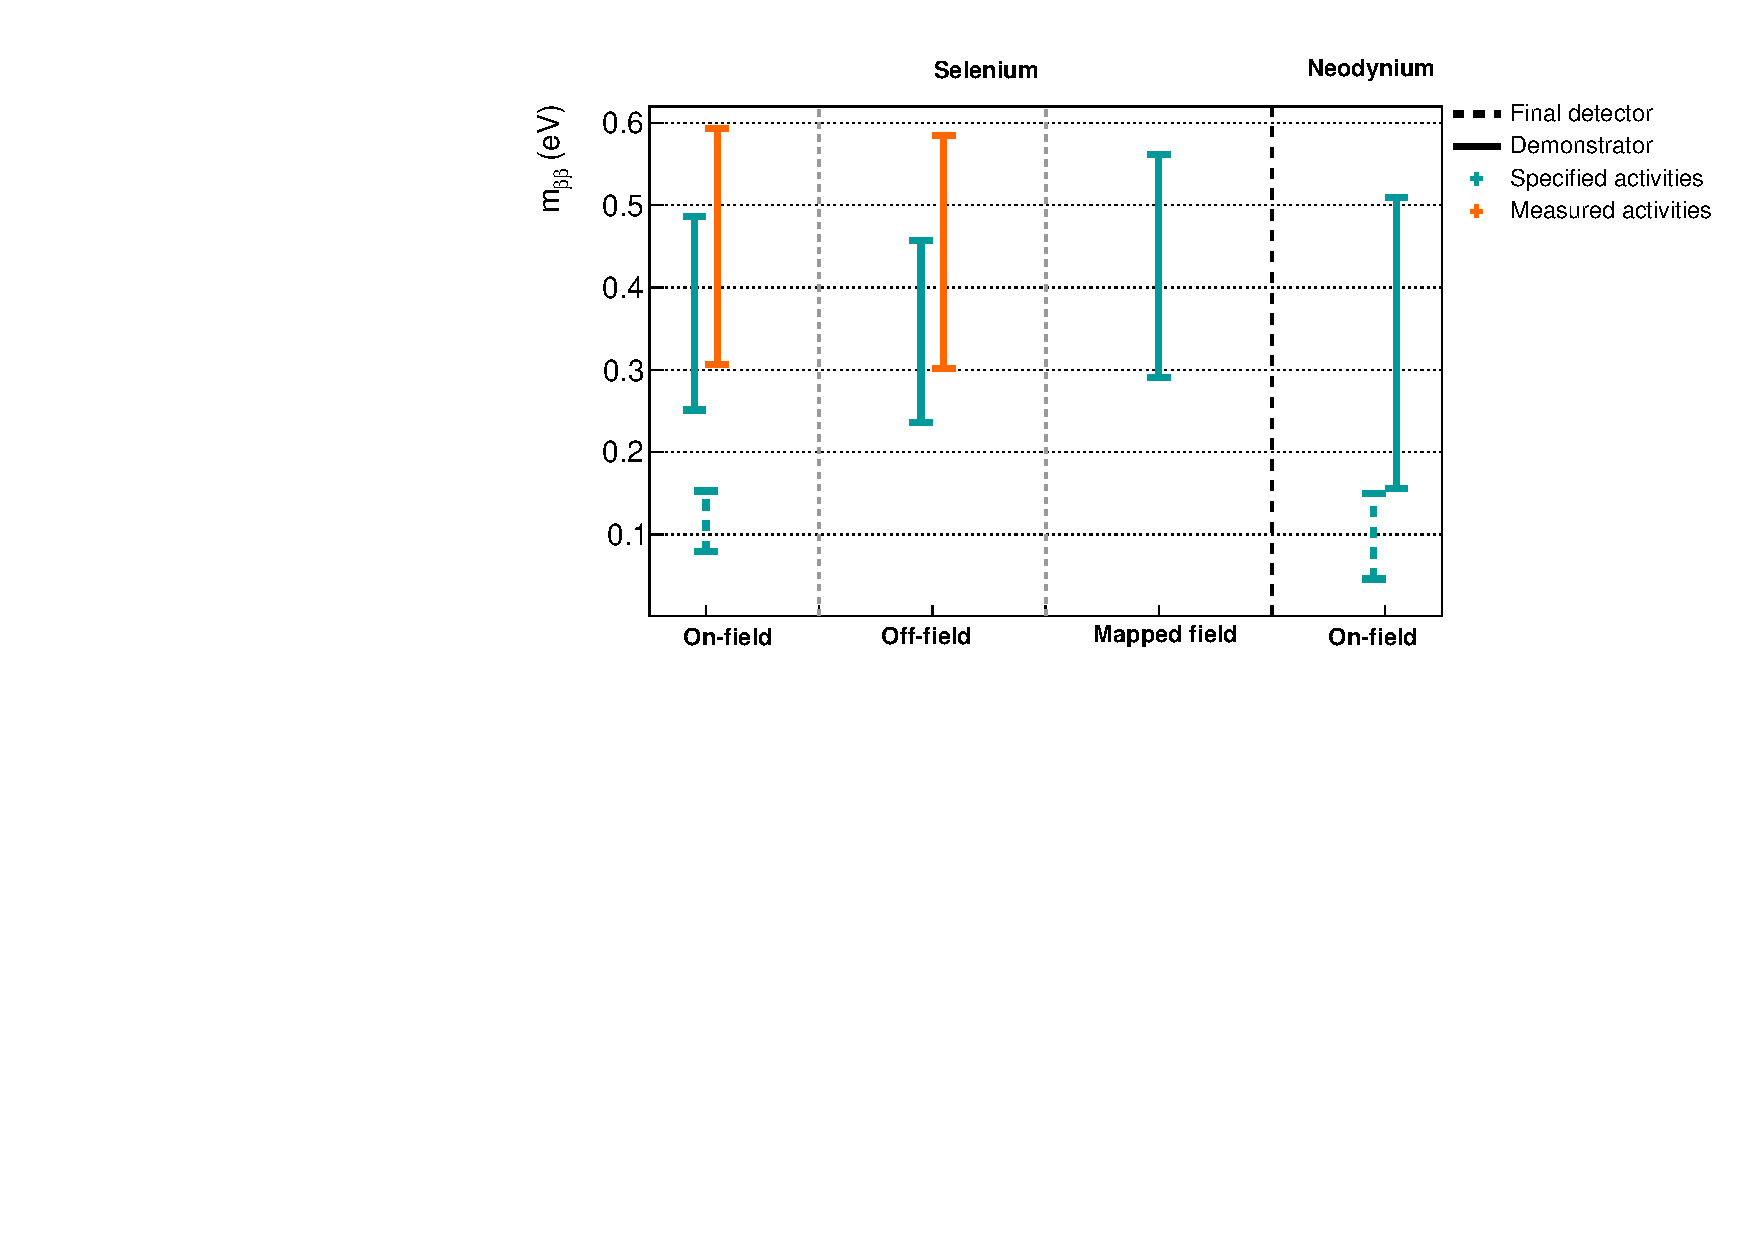
\includegraphics[width=1\textwidth]{Sensitivity/fig_sensitivity/final_mbb.pdf}
  \captionsetup{justification=centering}
  \caption{$\mbb$ limits.
    \label{subfig:summary_mbb}}
\end{subfigure}
\caption{Summary of limits set on $\Tbeta$ (a) and $\mbb$ (b) for each case dealt with in this chapter.
  First-order and optimised topological cut-offs have been applied.
  Regions of interest have been optimised for each case.
  \label{fig:final_t12}}
\end{figure}
